% !TeX root = surgery.tex
% !TeX encoding = UTF-8
% !TeX spellcheck = en_GB
\documentclass[12pt]{article} %taking out draft switches off marginal notes
\usepackage{../incremental_SS_Translation,gitver} % all customizations in this file
\addbibresource{../incremental_SS_Translation.bib} % putting this here lets TeXstudio find it.

\pagestyle{fancy}
\renewcommand{\sectionmark}[1]{\markboth{#1}{}} % set the \leftmark
\fancyhf{}
\fancyhead[R]{\relax} %predefined ()
\fancyhead[L]{\leftmark} % 1. sectionname
\fancyfoot[C]{\thepage}


\title{The \SS\ on the Plastic Surgery of the Ears and Nose:\\ The Nepalese 
Recension}

\author{Dominik Wujastyk \and
Jason Birch \and
Andrey Klebanov \and  
Madhu K. Parameswaran \and 
Madhusudan Rimal \and  
Deepro Chakraborty \and 
Harshal Bhatt \and  
Vandana Lele \and
Paras Mehta}
\date{\texttt{Draft of \today}\\ \copyright\     The authors.}

% Turn off Devanagari:
% \let\dev=\emph

\begin{document}
  
    % Manual hyphenation points for Sanskrit words and compounds.
% By Dominik Wujastyk.
% Copyright Dominik Wujastyk 2021.
% Released under a BY-SA Creative Commons license 
% (Attribution-ShareAlike 4.0 International http://creativecommons.org/licenses/by-sa/4.0/).
% This file is still actively growing, slowly but steadily (March 2021) .
%
% These special hyphenations have to be loaded after
% \begin{document}. See
% http://www.tug.org/pipermail/xetex/2008-July/010362.html
% Or use 
% \AtBeginDocument{% Manual hyphenation points for Sanskrit words and compounds.
% By Dominik Wujastyk.
% Copyright Dominik Wujastyk 2021.
% Released under a BY-SA Creative Commons license 
% (Attribution-ShareAlike 4.0 International http://creativecommons.org/licenses/by-sa/4.0/).
% This file is still actively growing, slowly but steadily (March 2021) .
%
% These special hyphenations have to be loaded after
% \begin{document}. See
% http://www.tug.org/pipermail/xetex/2008-July/010362.html
% Or use 
% \AtBeginDocument{% Manual hyphenation points for Sanskrit words and compounds.
% By Dominik Wujastyk.
% Copyright Dominik Wujastyk 2021.
% Released under a BY-SA Creative Commons license 
% (Attribution-ShareAlike 4.0 International http://creativecommons.org/licenses/by-sa/4.0/).
% This file is still actively growing, slowly but steadily (March 2021) .
%
% These special hyphenations have to be loaded after
% \begin{document}. See
% http://www.tug.org/pipermail/xetex/2008-July/010362.html
% Or use 
% \AtBeginDocument{\input{sanskrit-hyphenations}}% should work, but doesn't
% special hyphenations for Sanskrit words tagged in
% Polyglossia.
% *English,\textenglish{},text,and
% *Sanskrit,\textsanskrit{},text.
%
% English (see below for \textsanskrit)
%
\hyphenation{%
    dhanva-ntariṇopa-diṣ-ṭaḥ
    suśruta-nāma-dheyena
    tac-chiṣyeṇa
    kāśyapa-saṃ-hitā
    cikitsā-sthāna
    su-śruta-san-dīpana-bhāṣya
    dṛṣṭi-maṇḍala
    uc-chiṅga-na
    sarva-siddhānta-tattva-cūḍā-maṇi
    tulya-sau-vīrāñja-na
    indra-gopa
    śrī-mad-abhi-nava-guptā-cārya-vi-ra-cita-vi-vṛti-same-tam
    viśva-nātha
śrī-mad-devī-bhāga-vata-mahā-purāṇa
    siddhā-n-ta-sun-dara
    brāhma-sphuṭa-siddh-ānta
    bhū-ta-saṅ-khyā
    bhū-ta-saṃ-khyā
    kathi-ta-pada
    devī-bhā-ga-vata-purāṇa
    devī-bhā-ga-vata-mahā-purāṇa
    Siddhānta-saṃ-hitā-sāra-sam-uc-caya
    sau-ra-pau-rāṇi-ka-mata-sam-artha-na
    Pṛthū-da-ka-svā-min
    Brah-ma-gupta
    Brāh-ma-sphu-ṭa-siddhānta
    siddhānta-sun-dara
    vāsa-nā-bhāṣya
    catur-veda
    bhū-maṇḍala
    jñāna-rāja
    graha-gaṇi-ta-cintā-maṇi
    Śiṣya-dhī-vṛd-dhi-da-tan-tra
    brah-māṇḍa-pu-rā-ṇa
    kūr-ma-pu-rā-ṇa
    jam-bū-dvī-pa
    bhā-ga-vata-pu-rā-ṇa
    kupya-ka
    nandi-suttam
    nandi-sutta
    su-bodhiā-bāī
    asaṅ-khyāta
    saṅ-khyāta
    saṅ-khyā-pra-māṇa
    saṃ-khā-pamāṇa
    nemi-chandra
    anu-yoga-dvāra
    tattvārtha-vārtika
    aka-laṅka
    tri-loka-sāra
    gaṇi-ma-pra-māṇa
    gaṇi-ma-ppa-māṇa
    eka-pra-bhṛti
gaṇaṇā-saṃ-khā
gaṇaṇā-saṅ-khyā
dvi-pra-bhṛti
duppa-bhi-ti-saṃ-khā
vedanābhi-ghāta
Viṣṇu-dharmottara-pu-rāṇa
abhaya-deva-sūri-vi-racita-vṛtti-vi-bhūṣi-tam
abhi-dhar-ma
abhi-dhar-ma-ko-śa
abhi-dhar-ma-ko-śa-bhā-ṣya
abhi-dharma-kośa-bhāṣya
abhi-dharma-kośa-bhāṣyam
abhi-nava
abhyaṃ-karopāhva-vāsu-deva-śāstri-vi-ra-ci-ta-yā
ācārya-śrī-jina-vijayālekhitāgra-vacanālaṃ-kṛtaś-ca
ācāry-opā-hvena
ādhāra
adhi-kāra
adhi-kāras
ādi-nātha
agni-besha
agni-veśa
ahir-budhnya
ahir-budhnya-saṃ-hitā
aita-reya-brāhma-ṇa
akusī-dasya
amara-bharati
Amar-augha-pra-bo-dha
amṛ-ta-siddhi
ānanda-kanda
ānan-da-rā-ya
ānand-āśra-ma-mudraṇā-la-ya
ānand-āśra-ma-saṃ-skṛta-granth-āva-liḥ
anna-pāna-mūlā
anu-ban-dhya-lakṣaṇa-sam-anv-itās
anu-bhav-ād
anu-bhū-ta-viṣayā-sam-pra-moṣa
anu-bhū-ta-viṣayā-sam-pra-moṣaḥ
aparo-kṣā-nu-bhū-ti
app-proxi-mate-ly
ardha-rātrika-karaṇa
ārdha-rātrika-karaṇa
ariya-pary-esana-sutta
arun-dhatī
ārya-bhaṭa
ārya-bhaṭā-cārya-vi-racitam
ārya-bhaṭīya
ārya-bhaṭīyaṃ
ārya-lalita-vistara-nāma-mahā-yāna-sūtra
ārya-mañju-śrī-mūla-kalpa
ārya-mañju-śrī-mūla-kalpaḥ
asaṃ-pra-moṣa
aṣṭāṅga-hṛdaya-saṃ-hitā
aṣṭāṅga-saṃ-graha
asura-bhavana
aśva-ghoṣa
ātaṅka-darpaṇa-vyā-khyā-yā
atha-vā
ava-sāda-na
āyār-aṅga-suttaṃ
ayur-ved
ayur-veda
āyur-veda
āyur-veda-dīpikā
āyur-veda-dīpikā-vyā-khyayā
āyur-ve-da-ra-sā-yana
āyur-veda-sū-tra
ayur-vedic
āyur-vedic
ayur-yog
bādhirya
bahir-deśa-ka
bala-bhadra
bala-kot
bala-krishnan
bāla-kṛṣṇa
bau-dhā-yana-dhar-ma-sūtra
bel-valkar
bhadra-kālī-man-tra-vi-dhi-pra-karaṇa
bhadrā-sana
bhadrā-sanam
bha-ga-vat-pāda
bhaiṣajya-ratnāvalī
bhan-d-ar-kar
bhartṛhari-viracitaḥ
bhaṭṭā-cārya
bhaṭṭot-pala-vi-vṛti-sahitā
Bhiṣag-varāḍha-malla-vi-racita-dīpikā-Kāśī-rāma-vaidya-vi-raci-ta-gūḍhā-rtha-dīpikā-bhyāṃ
bhiṣag-varāḍha-malla-vi-racita-dīpikā-Kāśī-rāma-vaidya-vi-racita-gūḍhārtha-dīpikā-bhyāṃ
bhoja-deva-vi-raci-ta-rāja-mārtaṇḍā-bhi-dha-vṛtti-sam-e-tāni
bhu--va-na-dī-pa-ka
bīja-pallava
bi-kaner
bodhi-sat-tva-bhūmi
brahma-gupta
brahmā-nanda
brahmāṇḍa-mahā-purā-ṇa
brahmāṇḍa-mahā-purā-ṇam
brahma-randhra
brahma-siddh-ānta
brāhma-sphuṭa-siddh-ānta
brāhma-sphu-ṭa-siddhānta
brahma-vi-hāra
brahma-vi-hāras
brahma-yā-mala-tan-tra
Bra-ja-bhāṣā
bṛhad-āraṇya-ka
bṛhad-yā-trā
bṛhad-yogi-yājña-valkya-smṛti
bṛhad-yogī-yājña-valkya-smṛti
bṛhaj-jāta-kam
bṛhat-khe-carī-pra-kāśa
buddhi-tattva-pra-karaṇa
cak-ra-dat-ta
cakra-datta
cakra-pāṇi-datta
cā-luk-ya
caraka-prati-saṃ-s-kṛta
caraka-prati-saṃ-s-kṛte
caraka-saṃ-hitā
casam-ul-lasi-tāmaharṣiṇāsu-śrutenavi-raci-tāsu-śruta-saṃ-hitā
cau-kham-ba
cau-luk-yas
chandi-garh
chara-ka
cha-rīre
chatt-opa-dh-ya-ya
chau-kham-bha
chi-ki-tsi-ta
cid-ghanā-nanda-nātha
ci-ka-ner
com-men-taries
com-men-tary
com-pre-hen-sive-ly
daiva-jñālaṃ-kṛti
daiva-jñālaṅ-kṛti
dāmo-dara-sūnu-Śārṅga-dharācārya-vi-racitā
Dāmodara-sūnu-Śārṅga-dharācārya-vi-racitā
darśanā-ṅkur-ābhi-dhayā
das-gupta
deha-madhya
deha-saṃ-bhava-hetavaḥ
deva-datta
deva-nagari
deva-nāgarī
devā-sura-siddha-gaṇaiḥ
dha-ra-ni-dhar
dharma-megha
dharma-meghaḥ
dhru-vam
dhru-va-sya
dhru-va-yonir
dhyā-na-grahopa-deśā-dhyā-yaś
dṛḍha-śūla-yukta-rakta
dvy-ulbaṇaikolba-ṇ-aiḥ
four-fold
gan-dh-ā-ra
gārgīya-jyoti-ṣa
gārgya-ke-rala-nīla-kaṇṭha-so-ma-sutva-vi-racita-bhāṣyo-pe-tam
garuḍa-mahā-purāṇa
gaurī-kāñcali-kā-tan-tra
gau-tama
gauta-mādi-tra-yo-da-śa-smṛty-ātma-kaḥ
gheraṇḍa-saṃ-hitā
gorakṣa-śata-ka
go-tama
granth-ā-laya
grantha-mālā
gran-tha-śreṇiḥ
grāsa-pramāṇa
guru-maṇḍala-grantha-mālā
gyatso
hari-śāstrī
haṭhābhyāsa-paddhati
haṭha-ratnā-valī
Haṭha-saṅ-keta-candri-kā
haṭha-tattva-kau-mudī
haṭha-yoga
hāyana-rat-na
haya-ta-gran-tha
hema-pra-bha-sūri
hetu-lakṣaṇa-saṃ-sargād
hīna-madhyādhi-kaiś
hindī-vyā-khyā-vi-marśope-taḥ
hoern-le
ijya-rkṣa
ikka-vālaga
indra-dhvaja
indrāṇī-kalpa
indria
Īśāna-śiva-guru-deva-pad-dhati
jābāla-darśanopa-ni-ṣad
jadav-ji
jagan-nā-tha
jala-basti
jal-pa-kal-pa-tāru
jam-bū-dvī-pa-pra-jña-pti
jam-bū-dvī-pa-pra-jña-pti-sūtra
jana-pad-a-sya
jāta-ka-kar-ma-pad-dhati
jaya-siṃha
jinā-agama-grantha-mālā
jin-en-dra-bud-dhi
jīvan-muk-ti-vi-veka
jñā-na-nir-mala
jñā-na-nir-malaṃ
joga-pra-dīpya-kā
jya-rkṣe
Jyo-tiḥ-śās-tra
jyo-ti-ṣa-rāya
jyoti-ṣa-rāya
jyotiṣa-siddhānta-saṃ-graha
jyotiṣa-siddhānta-saṅ-graha
kāka-caṇḍīśvara-kal-pa-tan-tra
kakṣa-puṭa
kali-kāla-sarva-jña
kali-kāla-sarva-jña-śrī-hema-candrācārya-vi-raci-ta
kali-kāla-sarva-jña-śrī-hema-candrācārya-vi-raci-taḥ
kali-yuga
kal-pa
kal-pa-sthāna
kalyāṇa-kāraka
Kāmeśva-ra-siṃha-dara-bhaṅgā-saṃ-skṛta-viśva-vidyā-layaḥ
kapāla-bhāti
karaṇa-tilaka
kar-ma
kar-man
kāṭhaka-saṃ-hitā
kavia-rasu
kavi-raj
keśa-va-śāstrī
ke-vala--rāma
keva-la-rāma
khaṇḍa-khādyaka-tappā
khe-carī-vidyā
knowl-edge
kol-ka-ta
kriyā-krama-karī
kṛṣṇa-pakṣa
kṛtti-kā
kṛtti-kās
kubji-kā-mata-tantra
kula-pañji-kā
kul-karni
ku-māra-saṃ-bhava
kuṭi-pra-veśa
kuṭi-pra-veśika
lakṣ-mī-veṅ-kaṭ-e-ś-va-ra
lit-era-ture
lit-era-tures
locana-roga
mādha-va
mādhava-kara
mādhava-ni-dāna
mādhava-ni-dā-nam
madh-ūni
madhya
mādhyan-dina
madhye
mahā-bhāra-ta
mahā-deva
mahā-kavi-bhartṛ-hari-praṇīta-tvena
maha-mahopa-dhyaya
mahā-maho-pā-dhyā-ya-śrī-vi-jñā-na-bhikṣu-vi-raci-taṃ
mahā-mati-śrī-mādhava-kara-pra-ṇī-taṃ
mahā-mudrā
mahā-muni-śrī-mad-vyāsa-pra-ṇī-ta
mahā-muni-śrī-mad-vyāsa-pra-ṇī-taṃ
maharṣiṇā
maha-rṣi-pra-ṇīta-dharma-śāstra-saṃ-grahaḥ
Maha-rṣi-varya-śrī-yogi-yā-jña-valkya-śiṣya-vi-racitā
mahā-sacca-ka-sutta
mahā-sati-paṭṭhā-na-sutta
mahā-vra-ta
mahā-yāna-sūtrālaṅ-kāra
maitrāya-ṇī-saṃ-hitā
maktab-khānas
māla-jit
māli-nī-vijayot-tara-tan-tra
manaḥ-sam-ā-dhi
mānasol-lāsa
mānava-dharma-śāstra
mandāgni-doṣa
mannar-guḍi
mano-har-lal
mano-ratha-nandin
man-u-script
man-u-scripts
mataṅga-pārame-śvara
mater-ials
matsya-purāṇam
medh-ā-ti-thi
medhā-tithi
mithilā-stha
mithilā-stham
mithilā-sthaṃ
mṛgendra-tantra-vṛtti
mud-rā-yantr-ā-laye
muktā-pīḍa
mūla-pāṭha
muṇḍī-kalpa
mun-sh-ram
Nāda-bindū-pa-ni-ṣat
nāga-bodhi
nāga-buddhi
nakṣa-tra
nara-siṃha
nārā-yaṇa-dāsa
nārā-yaṇa-dāsa
nārā-yaṇa-kaṇṭha
nārā-yaṇa-paṇḍi-ta-kṛtā
nar-ra-tive
nata-rajan
nava-pañca-mayor
nava-re
naya-na-sukho-pā--dhyāya
ni-ban-dha-saṃ-grahā-khya-vyākhya-yā
niban-dha-san-graha
ni-dā-na
nidā-na-sthā-na-sya
ni-dāna-sthānasyaśrī-gaya-dāsācārya-vi-racitayānyāya-candri-kā-khya-pañjikā-vyā-khyayā
nir-anta-ra-pa-da-vyā-khyā
nir-guṇḍī-kalpa
nir-ṇaya-sā-gara
Nir-ṇaya-sāgara
nir-ṇa-ya-sā-gara-mudrā-yantrā-laye
nir-ṇa-ya-sā-ga-ra-yantr-āla-ya
nir-ṇaya-sā-gara-yantr-ā-laye
niśvāsa-kārikā
nīti-śṛṅgāra-vai-rāgyādi-nāmnāsamākhyā-tānāṃ
nityā-nanda
nya-grodha
nya-grodho
nyā-ya-candri-kā-khya-pañji-kā-vyā-khya-yā
nyāya-śās-tra
okaḥ-sātmya
okaḥ-sātmyam
okaḥ-sātmyaṃ
oka-sātmya
oka-sātmyam
oka-sātmyaṃ
oris-sa
oṣṭha-saṃ-puṭa
ousha-da-sala
padma-pra-bha-sūri
Padma-prā-bhṛ-ta-ka
padma-sva-sti-kārdha-candrādike
paitā-maha-siddhā-nta
pañca-karma
pañca-karman
pāñca-rātrā-gama
pañca-siddh-āntikā
paṅkti-śūla
Paraśu-rāma
paraśu-rāma
pari-likh-ya
pāśu-pata-sū-tra-bhāṣya
pātañ-jala-yoga-śās-tra
pātañ-jala-yoga-śās-tra-vi-varaṇa
pat-añ-jali
pat-na
pāva-suya
phiraṅgi-can-dra-cchedyo-pa-yogi-ka
pim-pal-gaon
pipal-gaon
pitta-śleṣ-man
pit-ta-śleṣ-ma-śoṇi-ta
pitta-śoṇi-ta
prā-cīna-rasa-granthaḥ
prā-cya
prā-cya-hindu-gran-tha-śreṇiḥ
prācya-vidyā-saṃ-śodhana-mandira
pra-dhān-in
pra-ka-shan
pra-kaṭa-mūṣā
pra-kṛ-ti-bhū-tāḥ
pra-mā-ṇa-vārt-tika
pra-ṇītā
pra-saṅ-khyāne
pra-śas-ta-pāda-bhāṣya
pra-śna-pra-dīpa
pra-śnārṇa-va-plava
praśnārṇava-plava
pra-śna-vai-ṣṇava
pra-śna-vaiṣṇava
prati-padyate
pra-yatna-śaithilyānan-ta-sam-āpatti-bhyām
prei-sen-danz
punar-vashu
puṇya-pattana
pūrṇi-mā-nta
raghu-nātha
rāja-kīya
rāja-kīya-mudraṇa-yantrā-laya
rāja-śe-khara
rajjv-ābhyas-ya
raj-put
rāj-put
rakta-mokṣa-na
rāma-candra-śāstrī
rāma-kṛṣṇa
rāma-kṛṣṇa-śāstri-ṇā
rama-su-bra-manian
rāmā-yaṇa
rasa-ratnā-kara
rasa-ratnākarāntar-ga-taś
rasa-ratna-sam-uc-caya
rasa-ratna-sam-uc-ca-yaḥ
rasa-vīry-auṣa-dha-pra-bhāvena
rasā-yana
rasendra-maṅgala
rasendra-maṅgalam
rāṣṭra-kūṭa
rāṣṭra-kūṭas
sādhana
śākalya-saṃ-hitā
śāla-grāma-kṛta
śāla-grāma-kṛta
sāmañña-pha-la-sutta
sāmañña-phala-sutta
sama-ran-gana-su-tra-dhara
samā-raṅga-ṇa-sū-tra-dhāra
sama-ra-siṃ-ha
sama-ra-siṃ-haḥ
sāmba-śiva-śāstri
same-taḥ
saṃ-hitā
śāṃ-ka-ra-bhāṣ-ya-sam-etā
sam-rāṭ
saṃ-rāṭ
Sam-rāṭ-siddhānta
Sam-rāṭ-siddhānta-kau-stu-bha
sam-rāṭ-siddhānta-kau-stu-bha
saṃ-sargam
saṃ-sargaṃ
saṃ-s-kṛta
saṃ-s-kṛta-pārasī-ka-pra-da-pra-kāśa
saṃ-śo-dhana
saṃ-śodhitā
saṃ-sthāna
sam-ullasitā
sam-ul-lasi-tam
saṃ-valitā
saṃ-valitā
śāndilyopa-ni-ṣad
śaṅ-kara
śaṅ-kara-bha-ga-vat-pāda
śaṅ-karā-cārya
san-kara-charya
Śaṅ-kara-nārā-yaṇa
sāṅ-kṛt-yā-yana
san-s-krit
śāra-dā-tila-ka-tan-tra
śa-raṅ-ga-deva
śār-dūla-karṇā-va-dāna
śār-dūla-karṇā-va-dāna
śā-rī-ra-sthāna
śārṅga-dhara-saṃ-hitā
Śārṅga-dhara-saṃ-hitā
sar-va-dar-śana-saṅ-gra-ha
sarva-kapha-ja
sarv-arthāvi-veka-khyā-ter
sar-va-śa-rīra-carās
sarva-siddhānta-rāja
Sarva-siddhā-nt-rāja
sarva-vyā-dhi-viṣāpa-ha
sarva-yoga-sam-uc-caya
sar-va-yogeśvareśva-ram
śāstrā-rambha-sam-artha-na
śatakatrayādi-subhāṣitasaṃgrahaḥ
sati-paṭṭhā-na-sutta
ṣaṭ-karma
ṣaṭ-karman
sat-karma-saṅ-graha
sat-karma-saṅ-grahaḥ
ṣaṭ-pañcā-śi-kā
saun-da-ra-nanda
sa-v-āī
schef-tel-o-witz
scholars
sharī-ra
sheth
sid-dha-man-tra
siddha-nanda-na-miśra
siddha-nanda-na-miśraḥ
siddha-nitya-nātha-pra-ṇītaḥ
Siddhānta-saṃ-hitā-sāra-sam-uc-caya
Siddhā-nta-sār-va-bhauma
siddhānta-sindhu
siddhānta-śiro-maṇ
Siddhānta-śiro-maṇi
Siddhā-nta-tat-tva-vi-veka
sid-dha-yoga
siddha-yoga
sid-dhi
sid-dhi-sthā-na
sid-dhi-sthāna
śikhi-sthāna
śiraḥ-karṇā-kṣi-vedana
śiro-bhūṣaṇam
Śivā-nanda-saras-vatī
śiva-saṃ-hitā
śiva-yo-ga-dī-pi-kā
ska-nda-pu-rā-ṇa
śleṣ-man
śleṣ-ma-śoni-ta
sodā-haraṇa-saṃ-s-kṛta-vyā-khyayā
śodha-ka-pusta-kaa
śoṇi-ta
spaṣ-ṭa-krānty-ādhi-kāra
śrī-cakra-pāṇi-datta
śrī-cakra-pāṇi-datta-viracitayā
śrī-ḍalhaṇācārya-vi-raci-tayāni-bandha-saṃ-grahākhya-vyā-khyayā
śrī-dayā-nanda
śrī-hari-kṛṣṇa-ni-bandha-bhava-nam
śrī-hema-candrā-cārya-vi-raci-taḥ
śrī-kaṇtha-dattā-bhyāṃ
śrī-kṛṣṇa-dāsa
śrī-kṛṣṇa-dāsa-śreṣṭhinā
śrīmac-chaṅ-kara-bhaga-vat-pāda-vi-raci-tā
śrī-mad-amara-siṃha-vi-racitam
śrī-mad-bha-ga-vad-gī-tā
śrī-mad-bhaṭṭot-pala-kṛta-saṃ-s-kṛta-ṭīkā-sahitam
śrī-mad-dvai-pā-yana-muni-pra-ṇītaṃ
śrī-mad-vāg-bhaṭa-vi-raci-tam
śrī-maṃ-trī-vi-jaya-siṃha-suta-maṃ-trī-teja-siṃhena
śrī-mat-kalyāṇa-varma-vi-racitā
śrī-mat-sāyaṇa-mādhavācārya-pra-ṇītaḥsarva-darśana-saṃ-grahaḥ
śrī-nitya-nātha-siddha-vi-raci-taḥ
śrī-rāja-śe-khara
śrī-śaṃ-karā-cārya-vi-raci-tam
śrī-vā-cas-pati-vaidya-vi-racita-yā
śrī-vatsa
śrī-veda-vyāsa-pra-ṇīta-mahā-bhā-ratāntar-ga-tā
śrī-veṅkaṭeś-vara
śrī-vi-jaya-rakṣi-ta
sruta-rakta
sruta-raktasya
stambha-karam
sthānāṅga-sūtra
sthira-sukha
sthira-sukham
stra-sthā-na
subhāṣitānāṃ
su-brah-man-ya
su-bra-man-ya
śukla-pakṣa
śukrā-srava
suk-than-kar
su-pariṣkṛta-saṃgrahaḥ
sura-bhi-pra-kash-an
sūrya-dāsa
sūrya-siddhānta
su-shru-ta
su-śru-ta
su-shru-ta-saṃ-hitā
su-śru-ta-saṃ-hitā
su-śru-tena
sutra
sūtra
sūtra-neti
sūtra-ni-dāna-śā-rīra-ci-ki-tsā-kal-pa-sthānot-tara-tan-trātma-kaḥ
sūtra-sthāna
su-varṇa-pra-bhāsot-tama-sū-tra
Su-var-ṇa-pra-bhās-ot-tama-sū-tra
su-varṇa-pra-bhāsotta-ma-sūtra
su-vistṛta-pari-cayātmikyāṅla-prastāvanā-vividha-pāṭhān-tara-pari-śiṣṭādi-sam-anvitaḥ
sva-bhāva-vyādhi-ni-vāraṇa-vi-śiṣṭ-auṣa-dha-cintakās
svā-bhāvika
svā-bhāvikās
sva-cchanda-tantra
śvetāśva-taropa-ni-ṣad
taila-sarpir-ma-dhūni
tait-tirīya-brāhma-ṇa
tājaka-muktā-valeḥ
tājika-kau-stu-bha
tājika-nīla-kaṇṭhī
tājika-yoga-sudhā-ni-dhi
tapo-dhana
tapo-dhanā
tārā-bhakti-su-dhārṇava
tārtīya-yoga-su-sudhā-ni-dhi
tegi-ccha
te-jaḥ-siṃ-ha
ṭhāṇ-āṅga-sutta
ṭīkā-bhyāṃ
ṭīkā-bhyāṃ
tiru-mantiram
tiru-ttoṇṭar-purāṇam
tiru-va-nanta-puram
trai-lok-ya
trai-lokya-pra-kāśa
tri-bhāga
tri-kam-ji
tri-pita-ka
tri-piṭa-ka
tri-vik-ra-mātma-jena
ud-ā-haraṇa
un-mārga-gama-na
upa-ca-ya-bala-varṇa-pra-sādādī-ni
upa-laghana
upa-ni-ṣads
upa-patt-ti
ut-sneha-na
utta-rā-dhya-ya-na
utta-rā-dhya-ya-na-sūtra
uttara-khaṇḍa-khādyaka
uttara-sthāna
uttara-tantra
vācas-pati-miśra-vi-racita-ṭīkā-saṃ-valita
vācas-pati-miśra-vi-racita-ṭīkā-saṃ-valita-vyā-sa-bhā-ṣya-sam-e-tāni
vag-bhata-rasa-ratna-sam-uc-caya
vāg-bhaṭa-rasa-ratna-sam-uc-caya
vaidya-vara-śrī-ḍalhaṇā-cārya-vi-racitayā
vai-śā-kha
vai-śeṣ-ika-sūtra
vāja-sa-neyi-saṃ-hitā
vājī-kara-ṇam
vākya-śeṣa
vākya-śeṣaḥ
vaṅga-sena
vaṅga-sena-saṃ-hitā
varā-ha-mihi-ra
vārāhī-kalpa
vā-rāṇa-seya
va-ra-na-si
var-mam
var-man
var-ṇa-saṃ-khyā
var-ṇa-saṅ-khyā
vā-si-ṣṭha
vasiṣṭha-saṃ-hitā
vā-siṣṭha-saṃ-hitā
Va-sistha-Sam-hita-Yoga-Kanda-With-Comm-ent-ary-Kai-valya-Dham
vastra-dhauti
vasu-bandhu
vāta-pit-ta
vāta-pit-ta-kapha
vāta-pit-ta-kapha-śoṇi-ta
vāta-pitta-kapha-śoṇita-san-nipāta-vai-ṣamya-ni-mittāḥ
vāta-pit-ta-śoṇi-ta
vāta-śleṣ-man
vāta-śleṣ-ma-śoṇi-ta
vāta-śoṇi-ta
vātā-tapika
vātsyā-ya-na
vāya-vīya-saṃ-hitā
vedāṅga-rāya
veezhi-nathan
venkat-raman
vid-vad-vara-śrī-gaṇeśa-daiva-jña-vi-racita
vidya-bhu-sana
vi-jaya-siṃ-ha
vi-jñāna-bhikṣu
Vijñāneśvara-vi-racita-mitākṣarā-vyā-khyā-sam-alaṅ-kṛtā
vi-mā-na
vi-mā-na-sthāna
vimāna-sthā-na
vi-racitā
vi-racita-yāmadhu-kośākhya-vyā-khya-yā
vi-recana
vishveshvar-anand
vi-śiṣṭ-āṃśena
vi-suddhi-magga
vi-vi-dha-tṛṇa-kāṣṭha-pāṣāṇa-pāṃ-su-loha-loṣṭāsthi-bāla-nakha-pūyā-srāva-duṣṭa-vraṇāntar-garbha-śalyo-ddharaṇārthaṃ
vṛd-dha-vṛd-dha-tara-vṛd-dha-tamaiḥ
vṛddha-vṛddha-tara-vṛddha-tamaiḥ
vṛnda-mādhava
vyāḍī-ya-pa-ri-bhā-ṣā-vṛtti
vyā-khya-yā
vy-akta-liṅgādi-dharma-yuk-te
vyā-sa-bhā-ṣya-sam-e-tāni
vyati-krāmati
Xiuyao
yādava-bhaṭṭa
yāda-va-śarma-ṇā
yādava-sūri
yājña-valkya-smṛti
yājña-valkya-smṛtiḥ
yantrā-dhyāya
Yantra-rāja-vicāra-viṃśā-dhyāyī
yavanā-cā-rya
yoga-bhā-ṣya-vyā-khyā-rūpaṃ
yoga-cintā-maṇi
yoga-cintā-maṇiḥ
yoga-ratnā-kara
yoga-sāra-mañjarī
yoga-sāra-sam-uc-caya
yoga-sāra-saṅ-graha
yoga-śikh-opa-ni-ṣat
yoga-tārā-valī
yoga-yājña-val-kya
yoga-yājña-valkya-gītāsūpa-ni-ṣatsu
yogi-yājña-valkya-smṛti
yoshi-mizu
yukta-bhava-deva
}
%%%%%%%%%%%%%%%%%%%%
%Sanskrit:
%%%%%%%%%%%%%%%%%%%%
\textsanskrit{\hyphenation{%
    dhanva-ntariṇopa-diṣ-ṭaḥ
suśruta-nāma-dheyena
tac-chiṣyeṇa
    su-śruta-san-dīpana-bhāṣya
    cikitsā-sthāna
tulya-sau-vīrāñjana
indra-gopa
dṛṣṭi-maṇḍala
uc-chiṅga-na
vi-vi-dha-tṛṇa-kāṣṭha-pāṣāṇa-pāṃ-su-loha-loṣṭāsthi-bāla-nakha-pūyā-srāva-duṣṭa-vraṇāntar-garbha-śalyo-ddharaṇārthaṃ
śrī-ḍalhaṇācārya-vi-raci-tayāni-bandha-saṃ-grahākhya-vyā-khyayā
ni-dāna-sthānasyaśrī-gaya-dāsācārya-vi-racitayānyāya-candri-kā-khya-pañjikā-vyā-khyayā
casam-ul-lasi-tāmaharṣiṇāsu-śrutenavi-raci-tāsu-śruta-saṃ-hitā
bhartṛhari-viracitaḥ
śatakatrayādi-subhāṣitasaṃgrahaḥ
mahā-kavi-bhartṛ-hari-praṇīta-tvena
nīti-śṛṅgāra-vai-rāgyādi-nāmnāsamākhyā-tānāṃ
subhāṣitānāṃ
su-pariṣkṛta-saṃgrahaḥ
su-vistṛta-pari-cayātmikyāṅla-prastāvanā-vividha-pāṭhān-tara-pari-śiṣṭādi-sam-anvitaḥ
ācārya-śrī-jina-vijayālekhitāgra-vacanālaṃ-kṛtaś-ca
abhaya-deva-sūri-vi-racita-vṛtti-vi-bhūṣi-tam
abhi-dhar-ma
abhi-dhar-ma-ko-śa
abhi-dhar-ma-ko-śa-bhā-ṣya
abhi-dharma-kośa-bhāṣyam
abhyaṃ-karopāhva-vāsu-deva-śāstri-vi-racita-yā
agni-veśa
āhā-ra-vi-hā-ra-pra-kṛ-tiṃ
ahir-budhnya
ahir-budhnya-saṃ-hitā
akusī-dasya
alter-na-tively
amara-bharati
amara-bhāratī
āmla
amlīkā
ānan-da-rā-ya
anna-mardanādi-bhiś
anu-bhav-ād
anu-bhū-ta-viṣayā-sam-pra-moṣa
anu-bhū-ta-viṣayā-sam-pra-moṣaḥ
anu-māna
anu-miti-mānasa-vāda
ariya-pary-esana-sutta
ārogya-śālā-karaṇā-sam-arthas
ārogya-śālām
ārogyāyopa-kal-pya
arś-āṃ-si
ar-tha
ar-thaḥ
ārya-bhaṭa
ārya-lalita-vistara-nāma-mahā-yāna-sūtra
ārya-mañju-śrī-mūla-kalpa
ārya-mañju-śrī-mūla-kalpaḥ
asaṃ-pra-moṣa
āsana
āsanam
āsanaṃ
asid-dhe
aṣṭāṅga-hṛdaya
aṣṭāṅga-hṛdaya-saṃ-hitā
aṣṭ-āṅga-saṅ-graha
aṣṭ-āṅgā-yur-veda
aśva-gan-dha-kalpa
aśva-ghoṣa
ātaṅka-darpaṇa
ātaṅka-darpaṇa-vyā-khyā-yā
atha-vā
ātu-r-ā-hā-ra-vi-hā-ra-pra-kṛ-tiṃ
aty-al-pam
auṣa-dha-pāvanādi-śālāś
ava-sāda-na
avic-chin-na-sam-pra-dāya-tvād
āyur-veda
āyur-veda-sāra
āyur-vedod-dhāra-ka-vaid-ya-pañc-ānana-vaid-ya-rat-na-rāja-vaid-ya-paṇḍi-ta-rā-ma-pra-sāda-vaid-yo-pādhyā-ya-vi-ra-ci-tā
bahir-deśa-ka
bala-bhadra
bāla-kṛṣṇa
bau-dhā-yana-dhar-ma-sūtra
bhadrā-sana
bhadrā-sanam
bha-ga-vad-gī-tā
bha-ga-vat-pāda
bhaṭṭot-pala-vi-vṛti-sahitā
bhṛtyāva-satha-saṃ-yuktām
bhū-miṃ
bhu--va-na-dī-pa-ka
bīja-pallava
bodhi-sat-tva-bhūmi
brāhmaṇa-pra-mukha-nānā-sat-tva-vyā-dhi-śānty-ar-tham
brāhmaṇa-pra-mukha-nānā-sat-tve-bhyo
brahmāṇḍa-mahā-purā-ṇa
brahmāṇḍa-mahā-purā-ṇam
brāhma-sphu-ṭa-siddhānta
brahma-vi-hāra
brahma-vi-hāras
bṛhad-āraṇya-ka
bṛhad-yā-trā
bṛhad-yogi-yājña-valkya-smṛti
bṛhad-yogī-yājña-valkya-smṛti
bṛhaj-jāta-kam
cak-ra-dat-ta
cak-ra-pā-ṇi-datta
cā-luk-ya
caraka-prati-saṃ-s-kṛta
caraka-prati-saṃ-s-kṛte
cara-ka-saṃ-hitā
ca-tur-thī-vi-bhak-ti
cau-kham-ba
cau-luk-yas
chau-kham-bha
chun-nam
cikit-sā-saṅ-gra-ha
daiva-jñālaṃ-kṛti
daiva-jñālaṅ-kṛti
darśa-nāṅkur-ābhi-dhayāvyā-khya-yā
deva-nagari
deva-nāgarī
dhar-ma-megha
dhar-ma-meghaḥ
dhyā-na-grahopa-deśā-dhyā-yaś
dṛṣṭ-ān-ta
dṛṣṭ-ār-tha
dvāra-tvam
evaṃ-gṛ-hī-tam
evaṃ-vi-dh-a-sya
gala-gaṇḍa
gala-gaṇḍādi-kar-tṛ-tvaṃ
gan-dh-ā-ra
gar-bha-śa-rī-ram
gaurī-kāñcali-kā-tan-tra
gauta-mādi-tra-yo-da-śa-smṛty-ātma-kaḥ
gheraṇḍa-saṃ-hitā
gran-tha-śreṇi
gran-tha-śreṇiḥ
guru-maṇḍala-grantha-mālā
hari-śāstrī
hari-śās-trī
haṭha-yoga
hāyana-rat-na
hema-pra-bha-sūri
hetv-ābhā-sa
hīna-mithy-āti-yoga
hīna-mithy-āti-yogena
hindī-vyā-khyā-vi-marśope-taḥ
hoern-le
idam
ijya-rkṣe
ikka-vālaga
ity-arthaḥ
jābāla-darśanopa-ni-ṣad
jal-pa-kal-pa-tāru
jam-bū-dvī-pa
jam-bū-dvī-pa-pra-jña-pti
jam-bū-dvī-pa-pra-jña-pti-sūtra
jāta-ka-kar-ma-pad-dhati
jinā-agama-grantha-mālā
jī-vā-nan-da-nam
jñā-na-nir-mala
jñā-na-nir-malaṃ
jya-rkṣe
kāka-caṇḍīśvara-kal-pa-tan-tra
kā-la-gar-bhā-śa-ya-pra-kṛ-tim
kā-la-gar-bhā-śa-ya-pra-kṛ-tiṃ
kali-kāla-sarva-jña
kali-kāla-sarva-jña-śrī-hema-candrācārya-vi-raci-ta
kali-kāla-sarva-jña-śrī-hema-candrācārya-vi-raci-taḥ
kali-yuga
kal-pa-sthāna
kar-ma
kar-man
kārt-snyena
katham
kāvya-mālā
keśa-va-śāstrī
kol-ka-ta
kṛṣṇa-pakṣa
kṛtti-kā
kṛtti-kās
kula-pañji-kā
ku-māra-saṃ-bhava
lab-dhāni
mada-na-phalam
mādha-va
Mādhava-karaaita-reya-brāhma-ṇa
Mādhava-ni-dāna
mādhava-ni-dā-nam
madhu-kośa
madhu-kośākhya-vyā-khya-yā
madhya
madhye
ma-hā-bhū-ta-vi-kā-ra-pra-kṛ-tiṃ
mahā-deva
mahā-mati-śrī-mādhava-kara-pra-ṇī-taṃ
mahā-muni-śrī-mad-vyāsa-pra-ṇī-ta
mahā-muni-śrī-mad-vyāsa-pra-ṇī-taṃ
maha-rṣi-pra-ṇīta-dharma-śāstra-saṃ-grahaḥ
mahā-sacca-ka-sutta
mahau-ṣadhi-pari-cchadāṃ
mahā-vra-ta
mahā-yāna-sūtrālaṅ-kāra
mano-ratha-nandin
matsya-purāṇam
me-dhā-ti-thi
medhā-tithi
mithilā-stha
mithilā-stham
mithilā-sthaṃ
mud-rā-yantr-ā-laye
muktā-pīḍa
mūla-pāṭha
nakṣa-tra
nandi-purāṇoktārogya-śālā-dāna-phala-prāpti-kāmo
nara-siṃha
nara-siṃha-bhāṣya
nārā-ya-ṇa-dāsa
nārā-yaṇa-kaṇṭha
nārā-yaṇa-paṇḍi-ta-kṛtā
nava-pañca-mayor
nidā-na-sthā-na-sya
ni-ghaṇ-ṭu
nir-anta-ra-pa-da-vyā-khyā
nir-ṇaya-sā-gara
nir-ṇaya-sā-gara-yantr-ā-laye
nirūha-vasti
niś-cala-kara
ni-yukta-vaidyāṃ
nya-grodha
nya-grodho
nyāya-śās-tra
nyāya-sū-tra-śaṃ-kar
okaḥ-sātmya
okaḥ-sātmyam
okaḥ-sātmyaṃ
oka-sātmya
oka-sātmyam
oka-sātmyaṃ
oṣṭha-saṃ-puṭa
ousha-da-sala
padma-pra-bha-sūri
padma-sva-sti-kārdha-candrādike
paitā-maha-siddhā-nta
pañca-karma
pañca-karma-bhava-rogāḥ
pañca-karmādhi-kāra
pañca-karma-vi-cāra
pāñca-rātrā-gama
pañca-siddh-āntikā
pari-bhāṣā
pari-likh-ya
pātañ-jala-yoga-śās-tra
pātañ-jala-yoga-śās-tra-vi-varaṇa
pat-añ-jali
pāṭī-gaṇita
pāva-suya
pim-pal-gaon
pipal-gaon
pit-ta-kṛt
pit-ta-śleṣma-ghna
pit-ta-śleṣma-medo-meha-hik-kā-śvā-sa-kā-sāti-sā-ra-cchardi-tṛṣṇā-kṛmi-vi-ṣa-pra-śa-ma-naṃ
prā-cya
prā-cya-hindu-gran-tha-śreṇiḥ
prācya-vidyā-saṃ-śodhana-mandira
pra-dhān-āṅ-gaṃ
pra-dhān-in
pra-ka-shan
pra-kṛ-ti
pra-kṛ-tiṃ
pra-mā-ṇa-vārt-tika
pra-saṅ-khyāne
pra-śas-ta-pāda-bhāṣya
pra-śna-pra-dīpa
pra-śnārṇa-va-plava
praśnārṇava-plava
pra-śna-vaiṣṇava
pra-śna-vai-ṣṇava
prati-padyate
pra-ty-akṣa
pra-yat-na-śai-thilyā-nan-ta-sam-ā-pat-ti-bhyām
pra-yat-na-śai-thilyā-nān-tya-sam-ā-pat-ti-bhyāṃ
pra-yatna-śai-thilya-sya
puṇya-pattana
pūrṇi-mā-nta
rāja-kīya
rajjv-ābhyas-ya
rāma-kṛṣṇa
rasa-ratnā-kara
rasa-vai-śeṣika-sūtra
rogi-svasthī-karaṇānu-ṣṭhāna-mātraṃ
rūkṣa-vasti
sād-guṇya
śākalya-saṃ-hitā
sam-ā-mnāya
sāmañña-pha-la-sutta
sama-ran-gana-su-tra-dhara
samā-raṅga-ṇa-sū-tra-dhāra
sama-ra-siṃ-ha
sama-ra-siṃ-haḥ
saṃ-hitā
sāṃ-sid-dhi-ka
saṃ-śo-dhana
sam-ul-lasi-tam
śāndilyopa-ni-ṣad
śaṅ-kara
śaṅ-kara-bha-ga-vat-pāda
Śaṅ-kara-nārā-yaṇa
saṅ-khyā
sāṅ-kṛt-yā-yana
san-s-krit
sap-tame
śāra-dā-tila-ka-tan-tra
śa-raṅ-ga-deva
śār-dūla-karṇā-va-dāna
śā-rī-ra
śā-rī-ra-sthāna
śārṅga-dhara
śārṅga-dhara-saṃ-hitā
sar-va
sarva-darśana-saṃ-grahaḥ
sar-va-dar-śāna-saṅ-gra-ha
sar-va-dar-śāna-saṅ-gra-haḥ
sarv-arthāvi-veka-khyā-ter
sar-va-tan-tra-sid-dhān-ta
sar-va-tan-tra-sid-dhān-taḥ
sarva-yoga-sam-uc-caya
sar-va-yogeśvareśva-ram
śāstrā-rambha-sam-artha-na
śāstrāram-bha-sam-arthana
ṣaṭ-pañcā-śi-kā
sat-tva
saunda-ra-na-nda
sid-dha
sid-dha-man-tra
sid-dha-man-trā-hvayo
sid-dha-man-tra-pra-kāśa
sid-dha-man-tra-pra-kāśaḥ
sid-dha-man-tra-pra-kāśaś
sid-dh-ān-ta
siddhānta-śiro-maṇ
sid-dha-yoga
sid-dhi-sthāna
śi-va-śar-ma-ṇā
ska-nda-pu-rā-ṇa
sneha-basty-upa-deśāt
sodā-haraṇa-saṃ-s-kṛta-vyā-khyayā
śodha-ka-pusta-kaṃ
śo-dha-na-ci-kitsā
so-ma-val-ka
śrī-mad-devī-bhāga-vata-mahā-purāṇa
srag-dharā-tārā-sto-tra
śrī-hari-kṛṣṇa-ni-bandha-bhava-nam
śrī-hema-candrā-cārya-vi-raci-taḥ
śrī-kaṇtha-datta
śrī-kaṇtha-dattā-bhyāṃ
śrī-kṛṣṇa-dāsa
śrī-mad-amara-siṃha-vi-racitam
śrī-mad-aruṇa-dat-ta-vi-ra-ci-tayā
śrī-mad-bhaṭṭot-pala-kṛta-saṃ-s-kṛta-ṭīkā-sahitam
śrī-mad-dvai-pā-yana-muni-pra-ṇītaṃ
śrī-mad-vāg-bha-ṭa-vi-ra-ci-tam
śrī-maṃ-trī-vi-jaya-siṃha-suta-maṃ-trī-teja-siṃhena
śrī-mat-kalyāṇa-varma-vi-racitā
śrīmat-sāyaṇa-mādhavācārya-pra-ṇītaḥ
śrī-vā-cas-pati-vaidya-vi-racita-yā
śrī-vatsa
śrī-vi-jaya-rakṣi-ta
sthānāṅga-sūtra
sthira-sukha
sthira-sukham
strī-niṣevaṇa
śukla-pakṣa
su-śru-ta-saṃ-hitā
sū-tra
sūtrārthānān-upa-patti-sūca-nāt
sūtra-sthāna
su-varṇa-pra-bhāsot-tama-sū-tra
svalpauṣadha-dāna-mā-tram
śvetāśva-taropa-ni-ṣad
tad-upa-karaṇa-tāmra-kaṭāha-kalasādi-pātra-pari-cchada-nānā-vidha-vyādhi-śānty-ucitauṣadha-gaṇa-yathokta-lakṣaṇa-vaidya-nānā-vidha-pari-cāraka-yutāṃ
tājaka-muktā-valeḥ
tājika-kau-stu-bha
tājika-nīla-kaṇṭhī
tājika-yoga-sudhā-ni-dhi
tāmra-paṭṭādi-li-khi-tāṃ
tan-nir-vāhāya
tapo-dhana
tapo-dhanā
tārā-bhakti-su-dhārṇava
tārtīya-yoga-su-sudhā-ni-dhi
tegi-ccha
te-jaḥ-siṃ-ha
trai-lok-ya
trai-lokya-pra-kāśa
tri-piṭa-ka
tri-var-gaḥ
un-mār-ga-gama-na
upa-de-śa
upa-patt-ti
ut-sneha-na
utta-rā-dhyā-ya-na
uttara-sthāna
uttara-tantra
vāchas-pati
vād-ā-valī
vai-śā-kha
vai-ta-raṇa-vasti
vai-ta-raṇok-ta-guṇa-gaṇa-yu-k-taṃ
vājī-kara-ṇam
vāk-patis
vākya-śeṣa
vākya-śeṣaḥ
varā-ha-mihi-ra
va-ra-na-si
vā-rā-ṇa-sī
var-mam
var-man
varṇa-sam-ā-mnāya
va-siṣṭha-saṃ-hitā
vā-siṣṭha-saṃ-hitā
vasu-bandhu
vasu-bandhu
vāta-ghna-pit-talāl-pa-ka-pha
vātsyā-ya-na
vidya-bhu-sana
vidyā-bhū-ṣaṇa
vi-jaya-siṃ-ha
vi-jñāna-bhikṣu
vi-kal-pa
vi-kamp-i-tum
vi-mā-na-sthāna
vi-racita-yā
vishveshvar-anand
vi-śiṣṭ-āṃśena
viṣṇu-dharmot-tara-purāṇa
viśrāma-gṛha-sahitā
vi-suddhi-magga
vopa-de-vīya-sid-dha-man-tra-pra-kāśe
vyādhi-pratī-kārār-tham
vyāḍī-ya-pa-ri-bhā-ṣā-vṛtti
vyati-krāmati
vy-ava-haranti
yādava-bhaṭṭa
yāda-va-śarma-ṇā
yādava-sūri
yājña-valkya-smṛti
yavanā-cā-rya
yoga-ratnā-kara
yoga-sāra-sam-uc-caya
yoga-sāra-sam-uc-cayaḥ
yoga-sūtra-vi-vara-ṇa
yoga-yājña-valkya
yoga-yājña-valkya-gītāsūpa-ni-ṣatsu
yoga-yājña-valkyaḥ
yogi-yājña-valkya-smṛti
yuk-tiḥ
yuk-tis
}}
\normalfontlatin
\endinput
}% should work, but doesn't
% special hyphenations for Sanskrit words tagged in
% Polyglossia.
% *English,\textenglish{},text,and
% *Sanskrit,\textsanskrit{},text.
%
% English (see below for \textsanskrit)
%
\hyphenation{%
    dhanva-ntariṇopa-diṣ-ṭaḥ
    suśruta-nāma-dheyena
    tac-chiṣyeṇa
    kāśyapa-saṃ-hitā
    cikitsā-sthāna
    su-śruta-san-dīpana-bhāṣya
    dṛṣṭi-maṇḍala
    uc-chiṅga-na
    sarva-siddhānta-tattva-cūḍā-maṇi
    tulya-sau-vīrāñja-na
    indra-gopa
    śrī-mad-abhi-nava-guptā-cārya-vi-ra-cita-vi-vṛti-same-tam
    viśva-nātha
śrī-mad-devī-bhāga-vata-mahā-purāṇa
    siddhā-n-ta-sun-dara
    brāhma-sphuṭa-siddh-ānta
    bhū-ta-saṅ-khyā
    bhū-ta-saṃ-khyā
    kathi-ta-pada
    devī-bhā-ga-vata-purāṇa
    devī-bhā-ga-vata-mahā-purāṇa
    Siddhānta-saṃ-hitā-sāra-sam-uc-caya
    sau-ra-pau-rāṇi-ka-mata-sam-artha-na
    Pṛthū-da-ka-svā-min
    Brah-ma-gupta
    Brāh-ma-sphu-ṭa-siddhānta
    siddhānta-sun-dara
    vāsa-nā-bhāṣya
    catur-veda
    bhū-maṇḍala
    jñāna-rāja
    graha-gaṇi-ta-cintā-maṇi
    Śiṣya-dhī-vṛd-dhi-da-tan-tra
    brah-māṇḍa-pu-rā-ṇa
    kūr-ma-pu-rā-ṇa
    jam-bū-dvī-pa
    bhā-ga-vata-pu-rā-ṇa
    kupya-ka
    nandi-suttam
    nandi-sutta
    su-bodhiā-bāī
    asaṅ-khyāta
    saṅ-khyāta
    saṅ-khyā-pra-māṇa
    saṃ-khā-pamāṇa
    nemi-chandra
    anu-yoga-dvāra
    tattvārtha-vārtika
    aka-laṅka
    tri-loka-sāra
    gaṇi-ma-pra-māṇa
    gaṇi-ma-ppa-māṇa
    eka-pra-bhṛti
gaṇaṇā-saṃ-khā
gaṇaṇā-saṅ-khyā
dvi-pra-bhṛti
duppa-bhi-ti-saṃ-khā
vedanābhi-ghāta
Viṣṇu-dharmottara-pu-rāṇa
abhaya-deva-sūri-vi-racita-vṛtti-vi-bhūṣi-tam
abhi-dhar-ma
abhi-dhar-ma-ko-śa
abhi-dhar-ma-ko-śa-bhā-ṣya
abhi-dharma-kośa-bhāṣya
abhi-dharma-kośa-bhāṣyam
abhi-nava
abhyaṃ-karopāhva-vāsu-deva-śāstri-vi-ra-ci-ta-yā
ācārya-śrī-jina-vijayālekhitāgra-vacanālaṃ-kṛtaś-ca
ācāry-opā-hvena
ādhāra
adhi-kāra
adhi-kāras
ādi-nātha
agni-besha
agni-veśa
ahir-budhnya
ahir-budhnya-saṃ-hitā
aita-reya-brāhma-ṇa
akusī-dasya
amara-bharati
Amar-augha-pra-bo-dha
amṛ-ta-siddhi
ānanda-kanda
ānan-da-rā-ya
ānand-āśra-ma-mudraṇā-la-ya
ānand-āśra-ma-saṃ-skṛta-granth-āva-liḥ
anna-pāna-mūlā
anu-ban-dhya-lakṣaṇa-sam-anv-itās
anu-bhav-ād
anu-bhū-ta-viṣayā-sam-pra-moṣa
anu-bhū-ta-viṣayā-sam-pra-moṣaḥ
aparo-kṣā-nu-bhū-ti
app-proxi-mate-ly
ardha-rātrika-karaṇa
ārdha-rātrika-karaṇa
ariya-pary-esana-sutta
arun-dhatī
ārya-bhaṭa
ārya-bhaṭā-cārya-vi-racitam
ārya-bhaṭīya
ārya-bhaṭīyaṃ
ārya-lalita-vistara-nāma-mahā-yāna-sūtra
ārya-mañju-śrī-mūla-kalpa
ārya-mañju-śrī-mūla-kalpaḥ
asaṃ-pra-moṣa
aṣṭāṅga-hṛdaya-saṃ-hitā
aṣṭāṅga-saṃ-graha
asura-bhavana
aśva-ghoṣa
ātaṅka-darpaṇa-vyā-khyā-yā
atha-vā
ava-sāda-na
āyār-aṅga-suttaṃ
ayur-ved
ayur-veda
āyur-veda
āyur-veda-dīpikā
āyur-veda-dīpikā-vyā-khyayā
āyur-ve-da-ra-sā-yana
āyur-veda-sū-tra
ayur-vedic
āyur-vedic
ayur-yog
bādhirya
bahir-deśa-ka
bala-bhadra
bala-kot
bala-krishnan
bāla-kṛṣṇa
bau-dhā-yana-dhar-ma-sūtra
bel-valkar
bhadra-kālī-man-tra-vi-dhi-pra-karaṇa
bhadrā-sana
bhadrā-sanam
bha-ga-vat-pāda
bhaiṣajya-ratnāvalī
bhan-d-ar-kar
bhartṛhari-viracitaḥ
bhaṭṭā-cārya
bhaṭṭot-pala-vi-vṛti-sahitā
Bhiṣag-varāḍha-malla-vi-racita-dīpikā-Kāśī-rāma-vaidya-vi-raci-ta-gūḍhā-rtha-dīpikā-bhyāṃ
bhiṣag-varāḍha-malla-vi-racita-dīpikā-Kāśī-rāma-vaidya-vi-racita-gūḍhārtha-dīpikā-bhyāṃ
bhoja-deva-vi-raci-ta-rāja-mārtaṇḍā-bhi-dha-vṛtti-sam-e-tāni
bhu--va-na-dī-pa-ka
bīja-pallava
bi-kaner
bodhi-sat-tva-bhūmi
brahma-gupta
brahmā-nanda
brahmāṇḍa-mahā-purā-ṇa
brahmāṇḍa-mahā-purā-ṇam
brahma-randhra
brahma-siddh-ānta
brāhma-sphuṭa-siddh-ānta
brāhma-sphu-ṭa-siddhānta
brahma-vi-hāra
brahma-vi-hāras
brahma-yā-mala-tan-tra
Bra-ja-bhāṣā
bṛhad-āraṇya-ka
bṛhad-yā-trā
bṛhad-yogi-yājña-valkya-smṛti
bṛhad-yogī-yājña-valkya-smṛti
bṛhaj-jāta-kam
bṛhat-khe-carī-pra-kāśa
buddhi-tattva-pra-karaṇa
cak-ra-dat-ta
cakra-datta
cakra-pāṇi-datta
cā-luk-ya
caraka-prati-saṃ-s-kṛta
caraka-prati-saṃ-s-kṛte
caraka-saṃ-hitā
casam-ul-lasi-tāmaharṣiṇāsu-śrutenavi-raci-tāsu-śruta-saṃ-hitā
cau-kham-ba
cau-luk-yas
chandi-garh
chara-ka
cha-rīre
chatt-opa-dh-ya-ya
chau-kham-bha
chi-ki-tsi-ta
cid-ghanā-nanda-nātha
ci-ka-ner
com-men-taries
com-men-tary
com-pre-hen-sive-ly
daiva-jñālaṃ-kṛti
daiva-jñālaṅ-kṛti
dāmo-dara-sūnu-Śārṅga-dharācārya-vi-racitā
Dāmodara-sūnu-Śārṅga-dharācārya-vi-racitā
darśanā-ṅkur-ābhi-dhayā
das-gupta
deha-madhya
deha-saṃ-bhava-hetavaḥ
deva-datta
deva-nagari
deva-nāgarī
devā-sura-siddha-gaṇaiḥ
dha-ra-ni-dhar
dharma-megha
dharma-meghaḥ
dhru-vam
dhru-va-sya
dhru-va-yonir
dhyā-na-grahopa-deśā-dhyā-yaś
dṛḍha-śūla-yukta-rakta
dvy-ulbaṇaikolba-ṇ-aiḥ
four-fold
gan-dh-ā-ra
gārgīya-jyoti-ṣa
gārgya-ke-rala-nīla-kaṇṭha-so-ma-sutva-vi-racita-bhāṣyo-pe-tam
garuḍa-mahā-purāṇa
gaurī-kāñcali-kā-tan-tra
gau-tama
gauta-mādi-tra-yo-da-śa-smṛty-ātma-kaḥ
gheraṇḍa-saṃ-hitā
gorakṣa-śata-ka
go-tama
granth-ā-laya
grantha-mālā
gran-tha-śreṇiḥ
grāsa-pramāṇa
guru-maṇḍala-grantha-mālā
gyatso
hari-śāstrī
haṭhābhyāsa-paddhati
haṭha-ratnā-valī
Haṭha-saṅ-keta-candri-kā
haṭha-tattva-kau-mudī
haṭha-yoga
hāyana-rat-na
haya-ta-gran-tha
hema-pra-bha-sūri
hetu-lakṣaṇa-saṃ-sargād
hīna-madhyādhi-kaiś
hindī-vyā-khyā-vi-marśope-taḥ
hoern-le
ijya-rkṣa
ikka-vālaga
indra-dhvaja
indrāṇī-kalpa
indria
Īśāna-śiva-guru-deva-pad-dhati
jābāla-darśanopa-ni-ṣad
jadav-ji
jagan-nā-tha
jala-basti
jal-pa-kal-pa-tāru
jam-bū-dvī-pa-pra-jña-pti
jam-bū-dvī-pa-pra-jña-pti-sūtra
jana-pad-a-sya
jāta-ka-kar-ma-pad-dhati
jaya-siṃha
jinā-agama-grantha-mālā
jin-en-dra-bud-dhi
jīvan-muk-ti-vi-veka
jñā-na-nir-mala
jñā-na-nir-malaṃ
joga-pra-dīpya-kā
jya-rkṣe
Jyo-tiḥ-śās-tra
jyo-ti-ṣa-rāya
jyoti-ṣa-rāya
jyotiṣa-siddhānta-saṃ-graha
jyotiṣa-siddhānta-saṅ-graha
kāka-caṇḍīśvara-kal-pa-tan-tra
kakṣa-puṭa
kali-kāla-sarva-jña
kali-kāla-sarva-jña-śrī-hema-candrācārya-vi-raci-ta
kali-kāla-sarva-jña-śrī-hema-candrācārya-vi-raci-taḥ
kali-yuga
kal-pa
kal-pa-sthāna
kalyāṇa-kāraka
Kāmeśva-ra-siṃha-dara-bhaṅgā-saṃ-skṛta-viśva-vidyā-layaḥ
kapāla-bhāti
karaṇa-tilaka
kar-ma
kar-man
kāṭhaka-saṃ-hitā
kavia-rasu
kavi-raj
keśa-va-śāstrī
ke-vala--rāma
keva-la-rāma
khaṇḍa-khādyaka-tappā
khe-carī-vidyā
knowl-edge
kol-ka-ta
kriyā-krama-karī
kṛṣṇa-pakṣa
kṛtti-kā
kṛtti-kās
kubji-kā-mata-tantra
kula-pañji-kā
kul-karni
ku-māra-saṃ-bhava
kuṭi-pra-veśa
kuṭi-pra-veśika
lakṣ-mī-veṅ-kaṭ-e-ś-va-ra
lit-era-ture
lit-era-tures
locana-roga
mādha-va
mādhava-kara
mādhava-ni-dāna
mādhava-ni-dā-nam
madh-ūni
madhya
mādhyan-dina
madhye
mahā-bhāra-ta
mahā-deva
mahā-kavi-bhartṛ-hari-praṇīta-tvena
maha-mahopa-dhyaya
mahā-maho-pā-dhyā-ya-śrī-vi-jñā-na-bhikṣu-vi-raci-taṃ
mahā-mati-śrī-mādhava-kara-pra-ṇī-taṃ
mahā-mudrā
mahā-muni-śrī-mad-vyāsa-pra-ṇī-ta
mahā-muni-śrī-mad-vyāsa-pra-ṇī-taṃ
maharṣiṇā
maha-rṣi-pra-ṇīta-dharma-śāstra-saṃ-grahaḥ
Maha-rṣi-varya-śrī-yogi-yā-jña-valkya-śiṣya-vi-racitā
mahā-sacca-ka-sutta
mahā-sati-paṭṭhā-na-sutta
mahā-vra-ta
mahā-yāna-sūtrālaṅ-kāra
maitrāya-ṇī-saṃ-hitā
maktab-khānas
māla-jit
māli-nī-vijayot-tara-tan-tra
manaḥ-sam-ā-dhi
mānasol-lāsa
mānava-dharma-śāstra
mandāgni-doṣa
mannar-guḍi
mano-har-lal
mano-ratha-nandin
man-u-script
man-u-scripts
mataṅga-pārame-śvara
mater-ials
matsya-purāṇam
medh-ā-ti-thi
medhā-tithi
mithilā-stha
mithilā-stham
mithilā-sthaṃ
mṛgendra-tantra-vṛtti
mud-rā-yantr-ā-laye
muktā-pīḍa
mūla-pāṭha
muṇḍī-kalpa
mun-sh-ram
Nāda-bindū-pa-ni-ṣat
nāga-bodhi
nāga-buddhi
nakṣa-tra
nara-siṃha
nārā-yaṇa-dāsa
nārā-yaṇa-dāsa
nārā-yaṇa-kaṇṭha
nārā-yaṇa-paṇḍi-ta-kṛtā
nar-ra-tive
nata-rajan
nava-pañca-mayor
nava-re
naya-na-sukho-pā--dhyāya
ni-ban-dha-saṃ-grahā-khya-vyākhya-yā
niban-dha-san-graha
ni-dā-na
nidā-na-sthā-na-sya
ni-dāna-sthānasyaśrī-gaya-dāsācārya-vi-racitayānyāya-candri-kā-khya-pañjikā-vyā-khyayā
nir-anta-ra-pa-da-vyā-khyā
nir-guṇḍī-kalpa
nir-ṇaya-sā-gara
Nir-ṇaya-sāgara
nir-ṇa-ya-sā-gara-mudrā-yantrā-laye
nir-ṇa-ya-sā-ga-ra-yantr-āla-ya
nir-ṇaya-sā-gara-yantr-ā-laye
niśvāsa-kārikā
nīti-śṛṅgāra-vai-rāgyādi-nāmnāsamākhyā-tānāṃ
nityā-nanda
nya-grodha
nya-grodho
nyā-ya-candri-kā-khya-pañji-kā-vyā-khya-yā
nyāya-śās-tra
okaḥ-sātmya
okaḥ-sātmyam
okaḥ-sātmyaṃ
oka-sātmya
oka-sātmyam
oka-sātmyaṃ
oris-sa
oṣṭha-saṃ-puṭa
ousha-da-sala
padma-pra-bha-sūri
Padma-prā-bhṛ-ta-ka
padma-sva-sti-kārdha-candrādike
paitā-maha-siddhā-nta
pañca-karma
pañca-karman
pāñca-rātrā-gama
pañca-siddh-āntikā
paṅkti-śūla
Paraśu-rāma
paraśu-rāma
pari-likh-ya
pāśu-pata-sū-tra-bhāṣya
pātañ-jala-yoga-śās-tra
pātañ-jala-yoga-śās-tra-vi-varaṇa
pat-añ-jali
pat-na
pāva-suya
phiraṅgi-can-dra-cchedyo-pa-yogi-ka
pim-pal-gaon
pipal-gaon
pitta-śleṣ-man
pit-ta-śleṣ-ma-śoṇi-ta
pitta-śoṇi-ta
prā-cīna-rasa-granthaḥ
prā-cya
prā-cya-hindu-gran-tha-śreṇiḥ
prācya-vidyā-saṃ-śodhana-mandira
pra-dhān-in
pra-ka-shan
pra-kaṭa-mūṣā
pra-kṛ-ti-bhū-tāḥ
pra-mā-ṇa-vārt-tika
pra-ṇītā
pra-saṅ-khyāne
pra-śas-ta-pāda-bhāṣya
pra-śna-pra-dīpa
pra-śnārṇa-va-plava
praśnārṇava-plava
pra-śna-vai-ṣṇava
pra-śna-vaiṣṇava
prati-padyate
pra-yatna-śaithilyānan-ta-sam-āpatti-bhyām
prei-sen-danz
punar-vashu
puṇya-pattana
pūrṇi-mā-nta
raghu-nātha
rāja-kīya
rāja-kīya-mudraṇa-yantrā-laya
rāja-śe-khara
rajjv-ābhyas-ya
raj-put
rāj-put
rakta-mokṣa-na
rāma-candra-śāstrī
rāma-kṛṣṇa
rāma-kṛṣṇa-śāstri-ṇā
rama-su-bra-manian
rāmā-yaṇa
rasa-ratnā-kara
rasa-ratnākarāntar-ga-taś
rasa-ratna-sam-uc-caya
rasa-ratna-sam-uc-ca-yaḥ
rasa-vīry-auṣa-dha-pra-bhāvena
rasā-yana
rasendra-maṅgala
rasendra-maṅgalam
rāṣṭra-kūṭa
rāṣṭra-kūṭas
sādhana
śākalya-saṃ-hitā
śāla-grāma-kṛta
śāla-grāma-kṛta
sāmañña-pha-la-sutta
sāmañña-phala-sutta
sama-ran-gana-su-tra-dhara
samā-raṅga-ṇa-sū-tra-dhāra
sama-ra-siṃ-ha
sama-ra-siṃ-haḥ
sāmba-śiva-śāstri
same-taḥ
saṃ-hitā
śāṃ-ka-ra-bhāṣ-ya-sam-etā
sam-rāṭ
saṃ-rāṭ
Sam-rāṭ-siddhānta
Sam-rāṭ-siddhānta-kau-stu-bha
sam-rāṭ-siddhānta-kau-stu-bha
saṃ-sargam
saṃ-sargaṃ
saṃ-s-kṛta
saṃ-s-kṛta-pārasī-ka-pra-da-pra-kāśa
saṃ-śo-dhana
saṃ-śodhitā
saṃ-sthāna
sam-ullasitā
sam-ul-lasi-tam
saṃ-valitā
saṃ-valitā
śāndilyopa-ni-ṣad
śaṅ-kara
śaṅ-kara-bha-ga-vat-pāda
śaṅ-karā-cārya
san-kara-charya
Śaṅ-kara-nārā-yaṇa
sāṅ-kṛt-yā-yana
san-s-krit
śāra-dā-tila-ka-tan-tra
śa-raṅ-ga-deva
śār-dūla-karṇā-va-dāna
śār-dūla-karṇā-va-dāna
śā-rī-ra-sthāna
śārṅga-dhara-saṃ-hitā
Śārṅga-dhara-saṃ-hitā
sar-va-dar-śana-saṅ-gra-ha
sarva-kapha-ja
sarv-arthāvi-veka-khyā-ter
sar-va-śa-rīra-carās
sarva-siddhānta-rāja
Sarva-siddhā-nt-rāja
sarva-vyā-dhi-viṣāpa-ha
sarva-yoga-sam-uc-caya
sar-va-yogeśvareśva-ram
śāstrā-rambha-sam-artha-na
śatakatrayādi-subhāṣitasaṃgrahaḥ
sati-paṭṭhā-na-sutta
ṣaṭ-karma
ṣaṭ-karman
sat-karma-saṅ-graha
sat-karma-saṅ-grahaḥ
ṣaṭ-pañcā-śi-kā
saun-da-ra-nanda
sa-v-āī
schef-tel-o-witz
scholars
sharī-ra
sheth
sid-dha-man-tra
siddha-nanda-na-miśra
siddha-nanda-na-miśraḥ
siddha-nitya-nātha-pra-ṇītaḥ
Siddhānta-saṃ-hitā-sāra-sam-uc-caya
Siddhā-nta-sār-va-bhauma
siddhānta-sindhu
siddhānta-śiro-maṇ
Siddhānta-śiro-maṇi
Siddhā-nta-tat-tva-vi-veka
sid-dha-yoga
siddha-yoga
sid-dhi
sid-dhi-sthā-na
sid-dhi-sthāna
śikhi-sthāna
śiraḥ-karṇā-kṣi-vedana
śiro-bhūṣaṇam
Śivā-nanda-saras-vatī
śiva-saṃ-hitā
śiva-yo-ga-dī-pi-kā
ska-nda-pu-rā-ṇa
śleṣ-man
śleṣ-ma-śoni-ta
sodā-haraṇa-saṃ-s-kṛta-vyā-khyayā
śodha-ka-pusta-kaa
śoṇi-ta
spaṣ-ṭa-krānty-ādhi-kāra
śrī-cakra-pāṇi-datta
śrī-cakra-pāṇi-datta-viracitayā
śrī-ḍalhaṇācārya-vi-raci-tayāni-bandha-saṃ-grahākhya-vyā-khyayā
śrī-dayā-nanda
śrī-hari-kṛṣṇa-ni-bandha-bhava-nam
śrī-hema-candrā-cārya-vi-raci-taḥ
śrī-kaṇtha-dattā-bhyāṃ
śrī-kṛṣṇa-dāsa
śrī-kṛṣṇa-dāsa-śreṣṭhinā
śrīmac-chaṅ-kara-bhaga-vat-pāda-vi-raci-tā
śrī-mad-amara-siṃha-vi-racitam
śrī-mad-bha-ga-vad-gī-tā
śrī-mad-bhaṭṭot-pala-kṛta-saṃ-s-kṛta-ṭīkā-sahitam
śrī-mad-dvai-pā-yana-muni-pra-ṇītaṃ
śrī-mad-vāg-bhaṭa-vi-raci-tam
śrī-maṃ-trī-vi-jaya-siṃha-suta-maṃ-trī-teja-siṃhena
śrī-mat-kalyāṇa-varma-vi-racitā
śrī-mat-sāyaṇa-mādhavācārya-pra-ṇītaḥsarva-darśana-saṃ-grahaḥ
śrī-nitya-nātha-siddha-vi-raci-taḥ
śrī-rāja-śe-khara
śrī-śaṃ-karā-cārya-vi-raci-tam
śrī-vā-cas-pati-vaidya-vi-racita-yā
śrī-vatsa
śrī-veda-vyāsa-pra-ṇīta-mahā-bhā-ratāntar-ga-tā
śrī-veṅkaṭeś-vara
śrī-vi-jaya-rakṣi-ta
sruta-rakta
sruta-raktasya
stambha-karam
sthānāṅga-sūtra
sthira-sukha
sthira-sukham
stra-sthā-na
subhāṣitānāṃ
su-brah-man-ya
su-bra-man-ya
śukla-pakṣa
śukrā-srava
suk-than-kar
su-pariṣkṛta-saṃgrahaḥ
sura-bhi-pra-kash-an
sūrya-dāsa
sūrya-siddhānta
su-shru-ta
su-śru-ta
su-shru-ta-saṃ-hitā
su-śru-ta-saṃ-hitā
su-śru-tena
sutra
sūtra
sūtra-neti
sūtra-ni-dāna-śā-rīra-ci-ki-tsā-kal-pa-sthānot-tara-tan-trātma-kaḥ
sūtra-sthāna
su-varṇa-pra-bhāsot-tama-sū-tra
Su-var-ṇa-pra-bhās-ot-tama-sū-tra
su-varṇa-pra-bhāsotta-ma-sūtra
su-vistṛta-pari-cayātmikyāṅla-prastāvanā-vividha-pāṭhān-tara-pari-śiṣṭādi-sam-anvitaḥ
sva-bhāva-vyādhi-ni-vāraṇa-vi-śiṣṭ-auṣa-dha-cintakās
svā-bhāvika
svā-bhāvikās
sva-cchanda-tantra
śvetāśva-taropa-ni-ṣad
taila-sarpir-ma-dhūni
tait-tirīya-brāhma-ṇa
tājaka-muktā-valeḥ
tājika-kau-stu-bha
tājika-nīla-kaṇṭhī
tājika-yoga-sudhā-ni-dhi
tapo-dhana
tapo-dhanā
tārā-bhakti-su-dhārṇava
tārtīya-yoga-su-sudhā-ni-dhi
tegi-ccha
te-jaḥ-siṃ-ha
ṭhāṇ-āṅga-sutta
ṭīkā-bhyāṃ
ṭīkā-bhyāṃ
tiru-mantiram
tiru-ttoṇṭar-purāṇam
tiru-va-nanta-puram
trai-lok-ya
trai-lokya-pra-kāśa
tri-bhāga
tri-kam-ji
tri-pita-ka
tri-piṭa-ka
tri-vik-ra-mātma-jena
ud-ā-haraṇa
un-mārga-gama-na
upa-ca-ya-bala-varṇa-pra-sādādī-ni
upa-laghana
upa-ni-ṣads
upa-patt-ti
ut-sneha-na
utta-rā-dhya-ya-na
utta-rā-dhya-ya-na-sūtra
uttara-khaṇḍa-khādyaka
uttara-sthāna
uttara-tantra
vācas-pati-miśra-vi-racita-ṭīkā-saṃ-valita
vācas-pati-miśra-vi-racita-ṭīkā-saṃ-valita-vyā-sa-bhā-ṣya-sam-e-tāni
vag-bhata-rasa-ratna-sam-uc-caya
vāg-bhaṭa-rasa-ratna-sam-uc-caya
vaidya-vara-śrī-ḍalhaṇā-cārya-vi-racitayā
vai-śā-kha
vai-śeṣ-ika-sūtra
vāja-sa-neyi-saṃ-hitā
vājī-kara-ṇam
vākya-śeṣa
vākya-śeṣaḥ
vaṅga-sena
vaṅga-sena-saṃ-hitā
varā-ha-mihi-ra
vārāhī-kalpa
vā-rāṇa-seya
va-ra-na-si
var-mam
var-man
var-ṇa-saṃ-khyā
var-ṇa-saṅ-khyā
vā-si-ṣṭha
vasiṣṭha-saṃ-hitā
vā-siṣṭha-saṃ-hitā
Va-sistha-Sam-hita-Yoga-Kanda-With-Comm-ent-ary-Kai-valya-Dham
vastra-dhauti
vasu-bandhu
vāta-pit-ta
vāta-pit-ta-kapha
vāta-pit-ta-kapha-śoṇi-ta
vāta-pitta-kapha-śoṇita-san-nipāta-vai-ṣamya-ni-mittāḥ
vāta-pit-ta-śoṇi-ta
vāta-śleṣ-man
vāta-śleṣ-ma-śoṇi-ta
vāta-śoṇi-ta
vātā-tapika
vātsyā-ya-na
vāya-vīya-saṃ-hitā
vedāṅga-rāya
veezhi-nathan
venkat-raman
vid-vad-vara-śrī-gaṇeśa-daiva-jña-vi-racita
vidya-bhu-sana
vi-jaya-siṃ-ha
vi-jñāna-bhikṣu
Vijñāneśvara-vi-racita-mitākṣarā-vyā-khyā-sam-alaṅ-kṛtā
vi-mā-na
vi-mā-na-sthāna
vimāna-sthā-na
vi-racitā
vi-racita-yāmadhu-kośākhya-vyā-khya-yā
vi-recana
vishveshvar-anand
vi-śiṣṭ-āṃśena
vi-suddhi-magga
vi-vi-dha-tṛṇa-kāṣṭha-pāṣāṇa-pāṃ-su-loha-loṣṭāsthi-bāla-nakha-pūyā-srāva-duṣṭa-vraṇāntar-garbha-śalyo-ddharaṇārthaṃ
vṛd-dha-vṛd-dha-tara-vṛd-dha-tamaiḥ
vṛddha-vṛddha-tara-vṛddha-tamaiḥ
vṛnda-mādhava
vyāḍī-ya-pa-ri-bhā-ṣā-vṛtti
vyā-khya-yā
vy-akta-liṅgādi-dharma-yuk-te
vyā-sa-bhā-ṣya-sam-e-tāni
vyati-krāmati
Xiuyao
yādava-bhaṭṭa
yāda-va-śarma-ṇā
yādava-sūri
yājña-valkya-smṛti
yājña-valkya-smṛtiḥ
yantrā-dhyāya
Yantra-rāja-vicāra-viṃśā-dhyāyī
yavanā-cā-rya
yoga-bhā-ṣya-vyā-khyā-rūpaṃ
yoga-cintā-maṇi
yoga-cintā-maṇiḥ
yoga-ratnā-kara
yoga-sāra-mañjarī
yoga-sāra-sam-uc-caya
yoga-sāra-saṅ-graha
yoga-śikh-opa-ni-ṣat
yoga-tārā-valī
yoga-yājña-val-kya
yoga-yājña-valkya-gītāsūpa-ni-ṣatsu
yogi-yājña-valkya-smṛti
yoshi-mizu
yukta-bhava-deva
}
%%%%%%%%%%%%%%%%%%%%
%Sanskrit:
%%%%%%%%%%%%%%%%%%%%
\textsanskrit{\hyphenation{%
    dhanva-ntariṇopa-diṣ-ṭaḥ
suśruta-nāma-dheyena
tac-chiṣyeṇa
    su-śruta-san-dīpana-bhāṣya
    cikitsā-sthāna
tulya-sau-vīrāñjana
indra-gopa
dṛṣṭi-maṇḍala
uc-chiṅga-na
vi-vi-dha-tṛṇa-kāṣṭha-pāṣāṇa-pāṃ-su-loha-loṣṭāsthi-bāla-nakha-pūyā-srāva-duṣṭa-vraṇāntar-garbha-śalyo-ddharaṇārthaṃ
śrī-ḍalhaṇācārya-vi-raci-tayāni-bandha-saṃ-grahākhya-vyā-khyayā
ni-dāna-sthānasyaśrī-gaya-dāsācārya-vi-racitayānyāya-candri-kā-khya-pañjikā-vyā-khyayā
casam-ul-lasi-tāmaharṣiṇāsu-śrutenavi-raci-tāsu-śruta-saṃ-hitā
bhartṛhari-viracitaḥ
śatakatrayādi-subhāṣitasaṃgrahaḥ
mahā-kavi-bhartṛ-hari-praṇīta-tvena
nīti-śṛṅgāra-vai-rāgyādi-nāmnāsamākhyā-tānāṃ
subhāṣitānāṃ
su-pariṣkṛta-saṃgrahaḥ
su-vistṛta-pari-cayātmikyāṅla-prastāvanā-vividha-pāṭhān-tara-pari-śiṣṭādi-sam-anvitaḥ
ācārya-śrī-jina-vijayālekhitāgra-vacanālaṃ-kṛtaś-ca
abhaya-deva-sūri-vi-racita-vṛtti-vi-bhūṣi-tam
abhi-dhar-ma
abhi-dhar-ma-ko-śa
abhi-dhar-ma-ko-śa-bhā-ṣya
abhi-dharma-kośa-bhāṣyam
abhyaṃ-karopāhva-vāsu-deva-śāstri-vi-racita-yā
agni-veśa
āhā-ra-vi-hā-ra-pra-kṛ-tiṃ
ahir-budhnya
ahir-budhnya-saṃ-hitā
akusī-dasya
alter-na-tively
amara-bharati
amara-bhāratī
āmla
amlīkā
ānan-da-rā-ya
anna-mardanādi-bhiś
anu-bhav-ād
anu-bhū-ta-viṣayā-sam-pra-moṣa
anu-bhū-ta-viṣayā-sam-pra-moṣaḥ
anu-māna
anu-miti-mānasa-vāda
ariya-pary-esana-sutta
ārogya-śālā-karaṇā-sam-arthas
ārogya-śālām
ārogyāyopa-kal-pya
arś-āṃ-si
ar-tha
ar-thaḥ
ārya-bhaṭa
ārya-lalita-vistara-nāma-mahā-yāna-sūtra
ārya-mañju-śrī-mūla-kalpa
ārya-mañju-śrī-mūla-kalpaḥ
asaṃ-pra-moṣa
āsana
āsanam
āsanaṃ
asid-dhe
aṣṭāṅga-hṛdaya
aṣṭāṅga-hṛdaya-saṃ-hitā
aṣṭ-āṅga-saṅ-graha
aṣṭ-āṅgā-yur-veda
aśva-gan-dha-kalpa
aśva-ghoṣa
ātaṅka-darpaṇa
ātaṅka-darpaṇa-vyā-khyā-yā
atha-vā
ātu-r-ā-hā-ra-vi-hā-ra-pra-kṛ-tiṃ
aty-al-pam
auṣa-dha-pāvanādi-śālāś
ava-sāda-na
avic-chin-na-sam-pra-dāya-tvād
āyur-veda
āyur-veda-sāra
āyur-vedod-dhāra-ka-vaid-ya-pañc-ānana-vaid-ya-rat-na-rāja-vaid-ya-paṇḍi-ta-rā-ma-pra-sāda-vaid-yo-pādhyā-ya-vi-ra-ci-tā
bahir-deśa-ka
bala-bhadra
bāla-kṛṣṇa
bau-dhā-yana-dhar-ma-sūtra
bhadrā-sana
bhadrā-sanam
bha-ga-vad-gī-tā
bha-ga-vat-pāda
bhaṭṭot-pala-vi-vṛti-sahitā
bhṛtyāva-satha-saṃ-yuktām
bhū-miṃ
bhu--va-na-dī-pa-ka
bīja-pallava
bodhi-sat-tva-bhūmi
brāhmaṇa-pra-mukha-nānā-sat-tva-vyā-dhi-śānty-ar-tham
brāhmaṇa-pra-mukha-nānā-sat-tve-bhyo
brahmāṇḍa-mahā-purā-ṇa
brahmāṇḍa-mahā-purā-ṇam
brāhma-sphu-ṭa-siddhānta
brahma-vi-hāra
brahma-vi-hāras
bṛhad-āraṇya-ka
bṛhad-yā-trā
bṛhad-yogi-yājña-valkya-smṛti
bṛhad-yogī-yājña-valkya-smṛti
bṛhaj-jāta-kam
cak-ra-dat-ta
cak-ra-pā-ṇi-datta
cā-luk-ya
caraka-prati-saṃ-s-kṛta
caraka-prati-saṃ-s-kṛte
cara-ka-saṃ-hitā
ca-tur-thī-vi-bhak-ti
cau-kham-ba
cau-luk-yas
chau-kham-bha
chun-nam
cikit-sā-saṅ-gra-ha
daiva-jñālaṃ-kṛti
daiva-jñālaṅ-kṛti
darśa-nāṅkur-ābhi-dhayāvyā-khya-yā
deva-nagari
deva-nāgarī
dhar-ma-megha
dhar-ma-meghaḥ
dhyā-na-grahopa-deśā-dhyā-yaś
dṛṣṭ-ān-ta
dṛṣṭ-ār-tha
dvāra-tvam
evaṃ-gṛ-hī-tam
evaṃ-vi-dh-a-sya
gala-gaṇḍa
gala-gaṇḍādi-kar-tṛ-tvaṃ
gan-dh-ā-ra
gar-bha-śa-rī-ram
gaurī-kāñcali-kā-tan-tra
gauta-mādi-tra-yo-da-śa-smṛty-ātma-kaḥ
gheraṇḍa-saṃ-hitā
gran-tha-śreṇi
gran-tha-śreṇiḥ
guru-maṇḍala-grantha-mālā
hari-śāstrī
hari-śās-trī
haṭha-yoga
hāyana-rat-na
hema-pra-bha-sūri
hetv-ābhā-sa
hīna-mithy-āti-yoga
hīna-mithy-āti-yogena
hindī-vyā-khyā-vi-marśope-taḥ
hoern-le
idam
ijya-rkṣe
ikka-vālaga
ity-arthaḥ
jābāla-darśanopa-ni-ṣad
jal-pa-kal-pa-tāru
jam-bū-dvī-pa
jam-bū-dvī-pa-pra-jña-pti
jam-bū-dvī-pa-pra-jña-pti-sūtra
jāta-ka-kar-ma-pad-dhati
jinā-agama-grantha-mālā
jī-vā-nan-da-nam
jñā-na-nir-mala
jñā-na-nir-malaṃ
jya-rkṣe
kāka-caṇḍīśvara-kal-pa-tan-tra
kā-la-gar-bhā-śa-ya-pra-kṛ-tim
kā-la-gar-bhā-śa-ya-pra-kṛ-tiṃ
kali-kāla-sarva-jña
kali-kāla-sarva-jña-śrī-hema-candrācārya-vi-raci-ta
kali-kāla-sarva-jña-śrī-hema-candrācārya-vi-raci-taḥ
kali-yuga
kal-pa-sthāna
kar-ma
kar-man
kārt-snyena
katham
kāvya-mālā
keśa-va-śāstrī
kol-ka-ta
kṛṣṇa-pakṣa
kṛtti-kā
kṛtti-kās
kula-pañji-kā
ku-māra-saṃ-bhava
lab-dhāni
mada-na-phalam
mādha-va
Mādhava-karaaita-reya-brāhma-ṇa
Mādhava-ni-dāna
mādhava-ni-dā-nam
madhu-kośa
madhu-kośākhya-vyā-khya-yā
madhya
madhye
ma-hā-bhū-ta-vi-kā-ra-pra-kṛ-tiṃ
mahā-deva
mahā-mati-śrī-mādhava-kara-pra-ṇī-taṃ
mahā-muni-śrī-mad-vyāsa-pra-ṇī-ta
mahā-muni-śrī-mad-vyāsa-pra-ṇī-taṃ
maha-rṣi-pra-ṇīta-dharma-śāstra-saṃ-grahaḥ
mahā-sacca-ka-sutta
mahau-ṣadhi-pari-cchadāṃ
mahā-vra-ta
mahā-yāna-sūtrālaṅ-kāra
mano-ratha-nandin
matsya-purāṇam
me-dhā-ti-thi
medhā-tithi
mithilā-stha
mithilā-stham
mithilā-sthaṃ
mud-rā-yantr-ā-laye
muktā-pīḍa
mūla-pāṭha
nakṣa-tra
nandi-purāṇoktārogya-śālā-dāna-phala-prāpti-kāmo
nara-siṃha
nara-siṃha-bhāṣya
nārā-ya-ṇa-dāsa
nārā-yaṇa-kaṇṭha
nārā-yaṇa-paṇḍi-ta-kṛtā
nava-pañca-mayor
nidā-na-sthā-na-sya
ni-ghaṇ-ṭu
nir-anta-ra-pa-da-vyā-khyā
nir-ṇaya-sā-gara
nir-ṇaya-sā-gara-yantr-ā-laye
nirūha-vasti
niś-cala-kara
ni-yukta-vaidyāṃ
nya-grodha
nya-grodho
nyāya-śās-tra
nyāya-sū-tra-śaṃ-kar
okaḥ-sātmya
okaḥ-sātmyam
okaḥ-sātmyaṃ
oka-sātmya
oka-sātmyam
oka-sātmyaṃ
oṣṭha-saṃ-puṭa
ousha-da-sala
padma-pra-bha-sūri
padma-sva-sti-kārdha-candrādike
paitā-maha-siddhā-nta
pañca-karma
pañca-karma-bhava-rogāḥ
pañca-karmādhi-kāra
pañca-karma-vi-cāra
pāñca-rātrā-gama
pañca-siddh-āntikā
pari-bhāṣā
pari-likh-ya
pātañ-jala-yoga-śās-tra
pātañ-jala-yoga-śās-tra-vi-varaṇa
pat-añ-jali
pāṭī-gaṇita
pāva-suya
pim-pal-gaon
pipal-gaon
pit-ta-kṛt
pit-ta-śleṣma-ghna
pit-ta-śleṣma-medo-meha-hik-kā-śvā-sa-kā-sāti-sā-ra-cchardi-tṛṣṇā-kṛmi-vi-ṣa-pra-śa-ma-naṃ
prā-cya
prā-cya-hindu-gran-tha-śreṇiḥ
prācya-vidyā-saṃ-śodhana-mandira
pra-dhān-āṅ-gaṃ
pra-dhān-in
pra-ka-shan
pra-kṛ-ti
pra-kṛ-tiṃ
pra-mā-ṇa-vārt-tika
pra-saṅ-khyāne
pra-śas-ta-pāda-bhāṣya
pra-śna-pra-dīpa
pra-śnārṇa-va-plava
praśnārṇava-plava
pra-śna-vaiṣṇava
pra-śna-vai-ṣṇava
prati-padyate
pra-ty-akṣa
pra-yat-na-śai-thilyā-nan-ta-sam-ā-pat-ti-bhyām
pra-yat-na-śai-thilyā-nān-tya-sam-ā-pat-ti-bhyāṃ
pra-yatna-śai-thilya-sya
puṇya-pattana
pūrṇi-mā-nta
rāja-kīya
rajjv-ābhyas-ya
rāma-kṛṣṇa
rasa-ratnā-kara
rasa-vai-śeṣika-sūtra
rogi-svasthī-karaṇānu-ṣṭhāna-mātraṃ
rūkṣa-vasti
sād-guṇya
śākalya-saṃ-hitā
sam-ā-mnāya
sāmañña-pha-la-sutta
sama-ran-gana-su-tra-dhara
samā-raṅga-ṇa-sū-tra-dhāra
sama-ra-siṃ-ha
sama-ra-siṃ-haḥ
saṃ-hitā
sāṃ-sid-dhi-ka
saṃ-śo-dhana
sam-ul-lasi-tam
śāndilyopa-ni-ṣad
śaṅ-kara
śaṅ-kara-bha-ga-vat-pāda
Śaṅ-kara-nārā-yaṇa
saṅ-khyā
sāṅ-kṛt-yā-yana
san-s-krit
sap-tame
śāra-dā-tila-ka-tan-tra
śa-raṅ-ga-deva
śār-dūla-karṇā-va-dāna
śā-rī-ra
śā-rī-ra-sthāna
śārṅga-dhara
śārṅga-dhara-saṃ-hitā
sar-va
sarva-darśana-saṃ-grahaḥ
sar-va-dar-śāna-saṅ-gra-ha
sar-va-dar-śāna-saṅ-gra-haḥ
sarv-arthāvi-veka-khyā-ter
sar-va-tan-tra-sid-dhān-ta
sar-va-tan-tra-sid-dhān-taḥ
sarva-yoga-sam-uc-caya
sar-va-yogeśvareśva-ram
śāstrā-rambha-sam-artha-na
śāstrāram-bha-sam-arthana
ṣaṭ-pañcā-śi-kā
sat-tva
saunda-ra-na-nda
sid-dha
sid-dha-man-tra
sid-dha-man-trā-hvayo
sid-dha-man-tra-pra-kāśa
sid-dha-man-tra-pra-kāśaḥ
sid-dha-man-tra-pra-kāśaś
sid-dh-ān-ta
siddhānta-śiro-maṇ
sid-dha-yoga
sid-dhi-sthāna
śi-va-śar-ma-ṇā
ska-nda-pu-rā-ṇa
sneha-basty-upa-deśāt
sodā-haraṇa-saṃ-s-kṛta-vyā-khyayā
śodha-ka-pusta-kaṃ
śo-dha-na-ci-kitsā
so-ma-val-ka
śrī-mad-devī-bhāga-vata-mahā-purāṇa
srag-dharā-tārā-sto-tra
śrī-hari-kṛṣṇa-ni-bandha-bhava-nam
śrī-hema-candrā-cārya-vi-raci-taḥ
śrī-kaṇtha-datta
śrī-kaṇtha-dattā-bhyāṃ
śrī-kṛṣṇa-dāsa
śrī-mad-amara-siṃha-vi-racitam
śrī-mad-aruṇa-dat-ta-vi-ra-ci-tayā
śrī-mad-bhaṭṭot-pala-kṛta-saṃ-s-kṛta-ṭīkā-sahitam
śrī-mad-dvai-pā-yana-muni-pra-ṇītaṃ
śrī-mad-vāg-bha-ṭa-vi-ra-ci-tam
śrī-maṃ-trī-vi-jaya-siṃha-suta-maṃ-trī-teja-siṃhena
śrī-mat-kalyāṇa-varma-vi-racitā
śrīmat-sāyaṇa-mādhavācārya-pra-ṇītaḥ
śrī-vā-cas-pati-vaidya-vi-racita-yā
śrī-vatsa
śrī-vi-jaya-rakṣi-ta
sthānāṅga-sūtra
sthira-sukha
sthira-sukham
strī-niṣevaṇa
śukla-pakṣa
su-śru-ta-saṃ-hitā
sū-tra
sūtrārthānān-upa-patti-sūca-nāt
sūtra-sthāna
su-varṇa-pra-bhāsot-tama-sū-tra
svalpauṣadha-dāna-mā-tram
śvetāśva-taropa-ni-ṣad
tad-upa-karaṇa-tāmra-kaṭāha-kalasādi-pātra-pari-cchada-nānā-vidha-vyādhi-śānty-ucitauṣadha-gaṇa-yathokta-lakṣaṇa-vaidya-nānā-vidha-pari-cāraka-yutāṃ
tājaka-muktā-valeḥ
tājika-kau-stu-bha
tājika-nīla-kaṇṭhī
tājika-yoga-sudhā-ni-dhi
tāmra-paṭṭādi-li-khi-tāṃ
tan-nir-vāhāya
tapo-dhana
tapo-dhanā
tārā-bhakti-su-dhārṇava
tārtīya-yoga-su-sudhā-ni-dhi
tegi-ccha
te-jaḥ-siṃ-ha
trai-lok-ya
trai-lokya-pra-kāśa
tri-piṭa-ka
tri-var-gaḥ
un-mār-ga-gama-na
upa-de-śa
upa-patt-ti
ut-sneha-na
utta-rā-dhyā-ya-na
uttara-sthāna
uttara-tantra
vāchas-pati
vād-ā-valī
vai-śā-kha
vai-ta-raṇa-vasti
vai-ta-raṇok-ta-guṇa-gaṇa-yu-k-taṃ
vājī-kara-ṇam
vāk-patis
vākya-śeṣa
vākya-śeṣaḥ
varā-ha-mihi-ra
va-ra-na-si
vā-rā-ṇa-sī
var-mam
var-man
varṇa-sam-ā-mnāya
va-siṣṭha-saṃ-hitā
vā-siṣṭha-saṃ-hitā
vasu-bandhu
vasu-bandhu
vāta-ghna-pit-talāl-pa-ka-pha
vātsyā-ya-na
vidya-bhu-sana
vidyā-bhū-ṣaṇa
vi-jaya-siṃ-ha
vi-jñāna-bhikṣu
vi-kal-pa
vi-kamp-i-tum
vi-mā-na-sthāna
vi-racita-yā
vishveshvar-anand
vi-śiṣṭ-āṃśena
viṣṇu-dharmot-tara-purāṇa
viśrāma-gṛha-sahitā
vi-suddhi-magga
vopa-de-vīya-sid-dha-man-tra-pra-kāśe
vyādhi-pratī-kārār-tham
vyāḍī-ya-pa-ri-bhā-ṣā-vṛtti
vyati-krāmati
vy-ava-haranti
yādava-bhaṭṭa
yāda-va-śarma-ṇā
yādava-sūri
yājña-valkya-smṛti
yavanā-cā-rya
yoga-ratnā-kara
yoga-sāra-sam-uc-caya
yoga-sāra-sam-uc-cayaḥ
yoga-sūtra-vi-vara-ṇa
yoga-yājña-valkya
yoga-yājña-valkya-gītāsūpa-ni-ṣatsu
yoga-yājña-valkyaḥ
yogi-yājña-valkya-smṛti
yuk-tiḥ
yuk-tis
}}
\normalfontlatin
\endinput
}% should work, but doesn't
% special hyphenations for Sanskrit words tagged in
% Polyglossia.
% *English,\textenglish{},text,and
% *Sanskrit,\textsanskrit{},text.
%
% English (see below for \textsanskrit)
%
\hyphenation{%
    dhanva-ntariṇopa-diṣ-ṭaḥ
    suśruta-nāma-dheyena
    tac-chiṣyeṇa
    kāśyapa-saṃ-hitā
    cikitsā-sthāna
    su-śruta-san-dīpana-bhāṣya
    dṛṣṭi-maṇḍala
    uc-chiṅga-na
    sarva-siddhānta-tattva-cūḍā-maṇi
    tulya-sau-vīrāñja-na
    indra-gopa
    śrī-mad-abhi-nava-guptā-cārya-vi-ra-cita-vi-vṛti-same-tam
    viśva-nātha
śrī-mad-devī-bhāga-vata-mahā-purāṇa
    siddhā-n-ta-sun-dara
    brāhma-sphuṭa-siddh-ānta
    bhū-ta-saṅ-khyā
    bhū-ta-saṃ-khyā
    kathi-ta-pada
    devī-bhā-ga-vata-purāṇa
    devī-bhā-ga-vata-mahā-purāṇa
    Siddhānta-saṃ-hitā-sāra-sam-uc-caya
    sau-ra-pau-rāṇi-ka-mata-sam-artha-na
    Pṛthū-da-ka-svā-min
    Brah-ma-gupta
    Brāh-ma-sphu-ṭa-siddhānta
    siddhānta-sun-dara
    vāsa-nā-bhāṣya
    catur-veda
    bhū-maṇḍala
    jñāna-rāja
    graha-gaṇi-ta-cintā-maṇi
    Śiṣya-dhī-vṛd-dhi-da-tan-tra
    brah-māṇḍa-pu-rā-ṇa
    kūr-ma-pu-rā-ṇa
    jam-bū-dvī-pa
    bhā-ga-vata-pu-rā-ṇa
    kupya-ka
    nandi-suttam
    nandi-sutta
    su-bodhiā-bāī
    asaṅ-khyāta
    saṅ-khyāta
    saṅ-khyā-pra-māṇa
    saṃ-khā-pamāṇa
    nemi-chandra
    anu-yoga-dvāra
    tattvārtha-vārtika
    aka-laṅka
    tri-loka-sāra
    gaṇi-ma-pra-māṇa
    gaṇi-ma-ppa-māṇa
    eka-pra-bhṛti
gaṇaṇā-saṃ-khā
gaṇaṇā-saṅ-khyā
dvi-pra-bhṛti
duppa-bhi-ti-saṃ-khā
vedanābhi-ghāta
Viṣṇu-dharmottara-pu-rāṇa
abhaya-deva-sūri-vi-racita-vṛtti-vi-bhūṣi-tam
abhi-dhar-ma
abhi-dhar-ma-ko-śa
abhi-dhar-ma-ko-śa-bhā-ṣya
abhi-dharma-kośa-bhāṣya
abhi-dharma-kośa-bhāṣyam
abhi-nava
abhyaṃ-karopāhva-vāsu-deva-śāstri-vi-ra-ci-ta-yā
ācārya-śrī-jina-vijayālekhitāgra-vacanālaṃ-kṛtaś-ca
ācāry-opā-hvena
ādhāra
adhi-kāra
adhi-kāras
ādi-nātha
agni-besha
agni-veśa
ahir-budhnya
ahir-budhnya-saṃ-hitā
aita-reya-brāhma-ṇa
akusī-dasya
amara-bharati
Amar-augha-pra-bo-dha
amṛ-ta-siddhi
ānanda-kanda
ānan-da-rā-ya
ānand-āśra-ma-mudraṇā-la-ya
ānand-āśra-ma-saṃ-skṛta-granth-āva-liḥ
anna-pāna-mūlā
anu-ban-dhya-lakṣaṇa-sam-anv-itās
anu-bhav-ād
anu-bhū-ta-viṣayā-sam-pra-moṣa
anu-bhū-ta-viṣayā-sam-pra-moṣaḥ
aparo-kṣā-nu-bhū-ti
app-proxi-mate-ly
ardha-rātrika-karaṇa
ārdha-rātrika-karaṇa
ariya-pary-esana-sutta
arun-dhatī
ārya-bhaṭa
ārya-bhaṭā-cārya-vi-racitam
ārya-bhaṭīya
ārya-bhaṭīyaṃ
ārya-lalita-vistara-nāma-mahā-yāna-sūtra
ārya-mañju-śrī-mūla-kalpa
ārya-mañju-śrī-mūla-kalpaḥ
asaṃ-pra-moṣa
aṣṭāṅga-hṛdaya-saṃ-hitā
aṣṭāṅga-saṃ-graha
asura-bhavana
aśva-ghoṣa
ātaṅka-darpaṇa-vyā-khyā-yā
atha-vā
ava-sāda-na
āyār-aṅga-suttaṃ
ayur-ved
ayur-veda
āyur-veda
āyur-veda-dīpikā
āyur-veda-dīpikā-vyā-khyayā
āyur-ve-da-ra-sā-yana
āyur-veda-sū-tra
ayur-vedic
āyur-vedic
ayur-yog
bādhirya
bahir-deśa-ka
bala-bhadra
bala-kot
bala-krishnan
bāla-kṛṣṇa
bau-dhā-yana-dhar-ma-sūtra
bel-valkar
bhadra-kālī-man-tra-vi-dhi-pra-karaṇa
bhadrā-sana
bhadrā-sanam
bha-ga-vat-pāda
bhaiṣajya-ratnāvalī
bhan-d-ar-kar
bhartṛhari-viracitaḥ
bhaṭṭā-cārya
bhaṭṭot-pala-vi-vṛti-sahitā
Bhiṣag-varāḍha-malla-vi-racita-dīpikā-Kāśī-rāma-vaidya-vi-raci-ta-gūḍhā-rtha-dīpikā-bhyāṃ
bhiṣag-varāḍha-malla-vi-racita-dīpikā-Kāśī-rāma-vaidya-vi-racita-gūḍhārtha-dīpikā-bhyāṃ
bhoja-deva-vi-raci-ta-rāja-mārtaṇḍā-bhi-dha-vṛtti-sam-e-tāni
bhu--va-na-dī-pa-ka
bīja-pallava
bi-kaner
bodhi-sat-tva-bhūmi
brahma-gupta
brahmā-nanda
brahmāṇḍa-mahā-purā-ṇa
brahmāṇḍa-mahā-purā-ṇam
brahma-randhra
brahma-siddh-ānta
brāhma-sphuṭa-siddh-ānta
brāhma-sphu-ṭa-siddhānta
brahma-vi-hāra
brahma-vi-hāras
brahma-yā-mala-tan-tra
Bra-ja-bhāṣā
bṛhad-āraṇya-ka
bṛhad-yā-trā
bṛhad-yogi-yājña-valkya-smṛti
bṛhad-yogī-yājña-valkya-smṛti
bṛhaj-jāta-kam
bṛhat-khe-carī-pra-kāśa
buddhi-tattva-pra-karaṇa
cak-ra-dat-ta
cakra-datta
cakra-pāṇi-datta
cā-luk-ya
caraka-prati-saṃ-s-kṛta
caraka-prati-saṃ-s-kṛte
caraka-saṃ-hitā
casam-ul-lasi-tāmaharṣiṇāsu-śrutenavi-raci-tāsu-śruta-saṃ-hitā
cau-kham-ba
cau-luk-yas
chandi-garh
chara-ka
cha-rīre
chatt-opa-dh-ya-ya
chau-kham-bha
chi-ki-tsi-ta
cid-ghanā-nanda-nātha
ci-ka-ner
com-men-taries
com-men-tary
com-pre-hen-sive-ly
daiva-jñālaṃ-kṛti
daiva-jñālaṅ-kṛti
dāmo-dara-sūnu-Śārṅga-dharācārya-vi-racitā
Dāmodara-sūnu-Śārṅga-dharācārya-vi-racitā
darśanā-ṅkur-ābhi-dhayā
das-gupta
deha-madhya
deha-saṃ-bhava-hetavaḥ
deva-datta
deva-nagari
deva-nāgarī
devā-sura-siddha-gaṇaiḥ
dha-ra-ni-dhar
dharma-megha
dharma-meghaḥ
dhru-vam
dhru-va-sya
dhru-va-yonir
dhyā-na-grahopa-deśā-dhyā-yaś
dṛḍha-śūla-yukta-rakta
dvy-ulbaṇaikolba-ṇ-aiḥ
four-fold
gan-dh-ā-ra
gārgīya-jyoti-ṣa
gārgya-ke-rala-nīla-kaṇṭha-so-ma-sutva-vi-racita-bhāṣyo-pe-tam
garuḍa-mahā-purāṇa
gaurī-kāñcali-kā-tan-tra
gau-tama
gauta-mādi-tra-yo-da-śa-smṛty-ātma-kaḥ
gheraṇḍa-saṃ-hitā
gorakṣa-śata-ka
go-tama
granth-ā-laya
grantha-mālā
gran-tha-śreṇiḥ
grāsa-pramāṇa
guru-maṇḍala-grantha-mālā
gyatso
hari-śāstrī
haṭhābhyāsa-paddhati
haṭha-ratnā-valī
Haṭha-saṅ-keta-candri-kā
haṭha-tattva-kau-mudī
haṭha-yoga
hāyana-rat-na
haya-ta-gran-tha
hema-pra-bha-sūri
hetu-lakṣaṇa-saṃ-sargād
hīna-madhyādhi-kaiś
hindī-vyā-khyā-vi-marśope-taḥ
hoern-le
ijya-rkṣa
ikka-vālaga
indra-dhvaja
indrāṇī-kalpa
indria
Īśāna-śiva-guru-deva-pad-dhati
jābāla-darśanopa-ni-ṣad
jadav-ji
jagan-nā-tha
jala-basti
jal-pa-kal-pa-tāru
jam-bū-dvī-pa-pra-jña-pti
jam-bū-dvī-pa-pra-jña-pti-sūtra
jana-pad-a-sya
jāta-ka-kar-ma-pad-dhati
jaya-siṃha
jinā-agama-grantha-mālā
jin-en-dra-bud-dhi
jīvan-muk-ti-vi-veka
jñā-na-nir-mala
jñā-na-nir-malaṃ
joga-pra-dīpya-kā
jya-rkṣe
Jyo-tiḥ-śās-tra
jyo-ti-ṣa-rāya
jyoti-ṣa-rāya
jyotiṣa-siddhānta-saṃ-graha
jyotiṣa-siddhānta-saṅ-graha
kāka-caṇḍīśvara-kal-pa-tan-tra
kakṣa-puṭa
kali-kāla-sarva-jña
kali-kāla-sarva-jña-śrī-hema-candrācārya-vi-raci-ta
kali-kāla-sarva-jña-śrī-hema-candrācārya-vi-raci-taḥ
kali-yuga
kal-pa
kal-pa-sthāna
kalyāṇa-kāraka
Kāmeśva-ra-siṃha-dara-bhaṅgā-saṃ-skṛta-viśva-vidyā-layaḥ
kapāla-bhāti
karaṇa-tilaka
kar-ma
kar-man
kāṭhaka-saṃ-hitā
kavia-rasu
kavi-raj
keśa-va-śāstrī
ke-vala--rāma
keva-la-rāma
khaṇḍa-khādyaka-tappā
khe-carī-vidyā
knowl-edge
kol-ka-ta
kriyā-krama-karī
kṛṣṇa-pakṣa
kṛtti-kā
kṛtti-kās
kubji-kā-mata-tantra
kula-pañji-kā
kul-karni
ku-māra-saṃ-bhava
kuṭi-pra-veśa
kuṭi-pra-veśika
lakṣ-mī-veṅ-kaṭ-e-ś-va-ra
lit-era-ture
lit-era-tures
locana-roga
mādha-va
mādhava-kara
mādhava-ni-dāna
mādhava-ni-dā-nam
madh-ūni
madhya
mādhyan-dina
madhye
mahā-bhāra-ta
mahā-deva
mahā-kavi-bhartṛ-hari-praṇīta-tvena
maha-mahopa-dhyaya
mahā-maho-pā-dhyā-ya-śrī-vi-jñā-na-bhikṣu-vi-raci-taṃ
mahā-mati-śrī-mādhava-kara-pra-ṇī-taṃ
mahā-mudrā
mahā-muni-śrī-mad-vyāsa-pra-ṇī-ta
mahā-muni-śrī-mad-vyāsa-pra-ṇī-taṃ
maharṣiṇā
maha-rṣi-pra-ṇīta-dharma-śāstra-saṃ-grahaḥ
Maha-rṣi-varya-śrī-yogi-yā-jña-valkya-śiṣya-vi-racitā
mahā-sacca-ka-sutta
mahā-sati-paṭṭhā-na-sutta
mahā-vra-ta
mahā-yāna-sūtrālaṅ-kāra
maitrāya-ṇī-saṃ-hitā
maktab-khānas
māla-jit
māli-nī-vijayot-tara-tan-tra
manaḥ-sam-ā-dhi
mānasol-lāsa
mānava-dharma-śāstra
mandāgni-doṣa
mannar-guḍi
mano-har-lal
mano-ratha-nandin
man-u-script
man-u-scripts
mataṅga-pārame-śvara
mater-ials
matsya-purāṇam
medh-ā-ti-thi
medhā-tithi
mithilā-stha
mithilā-stham
mithilā-sthaṃ
mṛgendra-tantra-vṛtti
mud-rā-yantr-ā-laye
muktā-pīḍa
mūla-pāṭha
muṇḍī-kalpa
mun-sh-ram
Nāda-bindū-pa-ni-ṣat
nāga-bodhi
nāga-buddhi
nakṣa-tra
nara-siṃha
nārā-yaṇa-dāsa
nārā-yaṇa-dāsa
nārā-yaṇa-kaṇṭha
nārā-yaṇa-paṇḍi-ta-kṛtā
nar-ra-tive
nata-rajan
nava-pañca-mayor
nava-re
naya-na-sukho-pā--dhyāya
ni-ban-dha-saṃ-grahā-khya-vyākhya-yā
niban-dha-san-graha
ni-dā-na
nidā-na-sthā-na-sya
ni-dāna-sthānasyaśrī-gaya-dāsācārya-vi-racitayānyāya-candri-kā-khya-pañjikā-vyā-khyayā
nir-anta-ra-pa-da-vyā-khyā
nir-guṇḍī-kalpa
nir-ṇaya-sā-gara
Nir-ṇaya-sāgara
nir-ṇa-ya-sā-gara-mudrā-yantrā-laye
nir-ṇa-ya-sā-ga-ra-yantr-āla-ya
nir-ṇaya-sā-gara-yantr-ā-laye
niśvāsa-kārikā
nīti-śṛṅgāra-vai-rāgyādi-nāmnāsamākhyā-tānāṃ
nityā-nanda
nya-grodha
nya-grodho
nyā-ya-candri-kā-khya-pañji-kā-vyā-khya-yā
nyāya-śās-tra
okaḥ-sātmya
okaḥ-sātmyam
okaḥ-sātmyaṃ
oka-sātmya
oka-sātmyam
oka-sātmyaṃ
oris-sa
oṣṭha-saṃ-puṭa
ousha-da-sala
padma-pra-bha-sūri
Padma-prā-bhṛ-ta-ka
padma-sva-sti-kārdha-candrādike
paitā-maha-siddhā-nta
pañca-karma
pañca-karman
pāñca-rātrā-gama
pañca-siddh-āntikā
paṅkti-śūla
Paraśu-rāma
paraśu-rāma
pari-likh-ya
pāśu-pata-sū-tra-bhāṣya
pātañ-jala-yoga-śās-tra
pātañ-jala-yoga-śās-tra-vi-varaṇa
pat-añ-jali
pat-na
pāva-suya
phiraṅgi-can-dra-cchedyo-pa-yogi-ka
pim-pal-gaon
pipal-gaon
pitta-śleṣ-man
pit-ta-śleṣ-ma-śoṇi-ta
pitta-śoṇi-ta
prā-cīna-rasa-granthaḥ
prā-cya
prā-cya-hindu-gran-tha-śreṇiḥ
prācya-vidyā-saṃ-śodhana-mandira
pra-dhān-in
pra-ka-shan
pra-kaṭa-mūṣā
pra-kṛ-ti-bhū-tāḥ
pra-mā-ṇa-vārt-tika
pra-ṇītā
pra-saṅ-khyāne
pra-śas-ta-pāda-bhāṣya
pra-śna-pra-dīpa
pra-śnārṇa-va-plava
praśnārṇava-plava
pra-śna-vai-ṣṇava
pra-śna-vaiṣṇava
prati-padyate
pra-yatna-śaithilyānan-ta-sam-āpatti-bhyām
prei-sen-danz
punar-vashu
puṇya-pattana
pūrṇi-mā-nta
raghu-nātha
rāja-kīya
rāja-kīya-mudraṇa-yantrā-laya
rāja-śe-khara
rajjv-ābhyas-ya
raj-put
rāj-put
rakta-mokṣa-na
rāma-candra-śāstrī
rāma-kṛṣṇa
rāma-kṛṣṇa-śāstri-ṇā
rama-su-bra-manian
rāmā-yaṇa
rasa-ratnā-kara
rasa-ratnākarāntar-ga-taś
rasa-ratna-sam-uc-caya
rasa-ratna-sam-uc-ca-yaḥ
rasa-vīry-auṣa-dha-pra-bhāvena
rasā-yana
rasendra-maṅgala
rasendra-maṅgalam
rāṣṭra-kūṭa
rāṣṭra-kūṭas
sādhana
śākalya-saṃ-hitā
śāla-grāma-kṛta
śāla-grāma-kṛta
sāmañña-pha-la-sutta
sāmañña-phala-sutta
sama-ran-gana-su-tra-dhara
samā-raṅga-ṇa-sū-tra-dhāra
sama-ra-siṃ-ha
sama-ra-siṃ-haḥ
sāmba-śiva-śāstri
same-taḥ
saṃ-hitā
śāṃ-ka-ra-bhāṣ-ya-sam-etā
sam-rāṭ
saṃ-rāṭ
Sam-rāṭ-siddhānta
Sam-rāṭ-siddhānta-kau-stu-bha
sam-rāṭ-siddhānta-kau-stu-bha
saṃ-sargam
saṃ-sargaṃ
saṃ-s-kṛta
saṃ-s-kṛta-pārasī-ka-pra-da-pra-kāśa
saṃ-śo-dhana
saṃ-śodhitā
saṃ-sthāna
sam-ullasitā
sam-ul-lasi-tam
saṃ-valitā
saṃ-valitā
śāndilyopa-ni-ṣad
śaṅ-kara
śaṅ-kara-bha-ga-vat-pāda
śaṅ-karā-cārya
san-kara-charya
Śaṅ-kara-nārā-yaṇa
sāṅ-kṛt-yā-yana
san-s-krit
śāra-dā-tila-ka-tan-tra
śa-raṅ-ga-deva
śār-dūla-karṇā-va-dāna
śār-dūla-karṇā-va-dāna
śā-rī-ra-sthāna
śārṅga-dhara-saṃ-hitā
Śārṅga-dhara-saṃ-hitā
sar-va-dar-śana-saṅ-gra-ha
sarva-kapha-ja
sarv-arthāvi-veka-khyā-ter
sar-va-śa-rīra-carās
sarva-siddhānta-rāja
Sarva-siddhā-nt-rāja
sarva-vyā-dhi-viṣāpa-ha
sarva-yoga-sam-uc-caya
sar-va-yogeśvareśva-ram
śāstrā-rambha-sam-artha-na
śatakatrayādi-subhāṣitasaṃgrahaḥ
sati-paṭṭhā-na-sutta
ṣaṭ-karma
ṣaṭ-karman
sat-karma-saṅ-graha
sat-karma-saṅ-grahaḥ
ṣaṭ-pañcā-śi-kā
saun-da-ra-nanda
sa-v-āī
schef-tel-o-witz
scholars
sharī-ra
sheth
sid-dha-man-tra
siddha-nanda-na-miśra
siddha-nanda-na-miśraḥ
siddha-nitya-nātha-pra-ṇītaḥ
Siddhānta-saṃ-hitā-sāra-sam-uc-caya
Siddhā-nta-sār-va-bhauma
siddhānta-sindhu
siddhānta-śiro-maṇ
Siddhānta-śiro-maṇi
Siddhā-nta-tat-tva-vi-veka
sid-dha-yoga
siddha-yoga
sid-dhi
sid-dhi-sthā-na
sid-dhi-sthāna
śikhi-sthāna
śiraḥ-karṇā-kṣi-vedana
śiro-bhūṣaṇam
Śivā-nanda-saras-vatī
śiva-saṃ-hitā
śiva-yo-ga-dī-pi-kā
ska-nda-pu-rā-ṇa
śleṣ-man
śleṣ-ma-śoni-ta
sodā-haraṇa-saṃ-s-kṛta-vyā-khyayā
śodha-ka-pusta-kaa
śoṇi-ta
spaṣ-ṭa-krānty-ādhi-kāra
śrī-cakra-pāṇi-datta
śrī-cakra-pāṇi-datta-viracitayā
śrī-ḍalhaṇācārya-vi-raci-tayāni-bandha-saṃ-grahākhya-vyā-khyayā
śrī-dayā-nanda
śrī-hari-kṛṣṇa-ni-bandha-bhava-nam
śrī-hema-candrā-cārya-vi-raci-taḥ
śrī-kaṇtha-dattā-bhyāṃ
śrī-kṛṣṇa-dāsa
śrī-kṛṣṇa-dāsa-śreṣṭhinā
śrīmac-chaṅ-kara-bhaga-vat-pāda-vi-raci-tā
śrī-mad-amara-siṃha-vi-racitam
śrī-mad-bha-ga-vad-gī-tā
śrī-mad-bhaṭṭot-pala-kṛta-saṃ-s-kṛta-ṭīkā-sahitam
śrī-mad-dvai-pā-yana-muni-pra-ṇītaṃ
śrī-mad-vāg-bhaṭa-vi-raci-tam
śrī-maṃ-trī-vi-jaya-siṃha-suta-maṃ-trī-teja-siṃhena
śrī-mat-kalyāṇa-varma-vi-racitā
śrī-mat-sāyaṇa-mādhavācārya-pra-ṇītaḥsarva-darśana-saṃ-grahaḥ
śrī-nitya-nātha-siddha-vi-raci-taḥ
śrī-rāja-śe-khara
śrī-śaṃ-karā-cārya-vi-raci-tam
śrī-vā-cas-pati-vaidya-vi-racita-yā
śrī-vatsa
śrī-veda-vyāsa-pra-ṇīta-mahā-bhā-ratāntar-ga-tā
śrī-veṅkaṭeś-vara
śrī-vi-jaya-rakṣi-ta
sruta-rakta
sruta-raktasya
stambha-karam
sthānāṅga-sūtra
sthira-sukha
sthira-sukham
stra-sthā-na
subhāṣitānāṃ
su-brah-man-ya
su-bra-man-ya
śukla-pakṣa
śukrā-srava
suk-than-kar
su-pariṣkṛta-saṃgrahaḥ
sura-bhi-pra-kash-an
sūrya-dāsa
sūrya-siddhānta
su-shru-ta
su-śru-ta
su-shru-ta-saṃ-hitā
su-śru-ta-saṃ-hitā
su-śru-tena
sutra
sūtra
sūtra-neti
sūtra-ni-dāna-śā-rīra-ci-ki-tsā-kal-pa-sthānot-tara-tan-trātma-kaḥ
sūtra-sthāna
su-varṇa-pra-bhāsot-tama-sū-tra
Su-var-ṇa-pra-bhās-ot-tama-sū-tra
su-varṇa-pra-bhāsotta-ma-sūtra
su-vistṛta-pari-cayātmikyāṅla-prastāvanā-vividha-pāṭhān-tara-pari-śiṣṭādi-sam-anvitaḥ
sva-bhāva-vyādhi-ni-vāraṇa-vi-śiṣṭ-auṣa-dha-cintakās
svā-bhāvika
svā-bhāvikās
sva-cchanda-tantra
śvetāśva-taropa-ni-ṣad
taila-sarpir-ma-dhūni
tait-tirīya-brāhma-ṇa
tājaka-muktā-valeḥ
tājika-kau-stu-bha
tājika-nīla-kaṇṭhī
tājika-yoga-sudhā-ni-dhi
tapo-dhana
tapo-dhanā
tārā-bhakti-su-dhārṇava
tārtīya-yoga-su-sudhā-ni-dhi
tegi-ccha
te-jaḥ-siṃ-ha
ṭhāṇ-āṅga-sutta
ṭīkā-bhyāṃ
ṭīkā-bhyāṃ
tiru-mantiram
tiru-ttoṇṭar-purāṇam
tiru-va-nanta-puram
trai-lok-ya
trai-lokya-pra-kāśa
tri-bhāga
tri-kam-ji
tri-pita-ka
tri-piṭa-ka
tri-vik-ra-mātma-jena
ud-ā-haraṇa
un-mārga-gama-na
upa-ca-ya-bala-varṇa-pra-sādādī-ni
upa-laghana
upa-ni-ṣads
upa-patt-ti
ut-sneha-na
utta-rā-dhya-ya-na
utta-rā-dhya-ya-na-sūtra
uttara-khaṇḍa-khādyaka
uttara-sthāna
uttara-tantra
vācas-pati-miśra-vi-racita-ṭīkā-saṃ-valita
vācas-pati-miśra-vi-racita-ṭīkā-saṃ-valita-vyā-sa-bhā-ṣya-sam-e-tāni
vag-bhata-rasa-ratna-sam-uc-caya
vāg-bhaṭa-rasa-ratna-sam-uc-caya
vaidya-vara-śrī-ḍalhaṇā-cārya-vi-racitayā
vai-śā-kha
vai-śeṣ-ika-sūtra
vāja-sa-neyi-saṃ-hitā
vājī-kara-ṇam
vākya-śeṣa
vākya-śeṣaḥ
vaṅga-sena
vaṅga-sena-saṃ-hitā
varā-ha-mihi-ra
vārāhī-kalpa
vā-rāṇa-seya
va-ra-na-si
var-mam
var-man
var-ṇa-saṃ-khyā
var-ṇa-saṅ-khyā
vā-si-ṣṭha
vasiṣṭha-saṃ-hitā
vā-siṣṭha-saṃ-hitā
Va-sistha-Sam-hita-Yoga-Kanda-With-Comm-ent-ary-Kai-valya-Dham
vastra-dhauti
vasu-bandhu
vāta-pit-ta
vāta-pit-ta-kapha
vāta-pit-ta-kapha-śoṇi-ta
vāta-pitta-kapha-śoṇita-san-nipāta-vai-ṣamya-ni-mittāḥ
vāta-pit-ta-śoṇi-ta
vāta-śleṣ-man
vāta-śleṣ-ma-śoṇi-ta
vāta-śoṇi-ta
vātā-tapika
vātsyā-ya-na
vāya-vīya-saṃ-hitā
vedāṅga-rāya
veezhi-nathan
venkat-raman
vid-vad-vara-śrī-gaṇeśa-daiva-jña-vi-racita
vidya-bhu-sana
vi-jaya-siṃ-ha
vi-jñāna-bhikṣu
Vijñāneśvara-vi-racita-mitākṣarā-vyā-khyā-sam-alaṅ-kṛtā
vi-mā-na
vi-mā-na-sthāna
vimāna-sthā-na
vi-racitā
vi-racita-yāmadhu-kośākhya-vyā-khya-yā
vi-recana
vishveshvar-anand
vi-śiṣṭ-āṃśena
vi-suddhi-magga
vi-vi-dha-tṛṇa-kāṣṭha-pāṣāṇa-pāṃ-su-loha-loṣṭāsthi-bāla-nakha-pūyā-srāva-duṣṭa-vraṇāntar-garbha-śalyo-ddharaṇārthaṃ
vṛd-dha-vṛd-dha-tara-vṛd-dha-tamaiḥ
vṛddha-vṛddha-tara-vṛddha-tamaiḥ
vṛnda-mādhava
vyāḍī-ya-pa-ri-bhā-ṣā-vṛtti
vyā-khya-yā
vy-akta-liṅgādi-dharma-yuk-te
vyā-sa-bhā-ṣya-sam-e-tāni
vyati-krāmati
Xiuyao
yādava-bhaṭṭa
yāda-va-śarma-ṇā
yādava-sūri
yājña-valkya-smṛti
yājña-valkya-smṛtiḥ
yantrā-dhyāya
Yantra-rāja-vicāra-viṃśā-dhyāyī
yavanā-cā-rya
yoga-bhā-ṣya-vyā-khyā-rūpaṃ
yoga-cintā-maṇi
yoga-cintā-maṇiḥ
yoga-ratnā-kara
yoga-sāra-mañjarī
yoga-sāra-sam-uc-caya
yoga-sāra-saṅ-graha
yoga-śikh-opa-ni-ṣat
yoga-tārā-valī
yoga-yājña-val-kya
yoga-yājña-valkya-gītāsūpa-ni-ṣatsu
yogi-yājña-valkya-smṛti
yoshi-mizu
yukta-bhava-deva
}
%%%%%%%%%%%%%%%%%%%%
%Sanskrit:
%%%%%%%%%%%%%%%%%%%%
\textsanskrit{\hyphenation{%
    dhanva-ntariṇopa-diṣ-ṭaḥ
suśruta-nāma-dheyena
tac-chiṣyeṇa
    su-śruta-san-dīpana-bhāṣya
    cikitsā-sthāna
tulya-sau-vīrāñjana
indra-gopa
dṛṣṭi-maṇḍala
uc-chiṅga-na
vi-vi-dha-tṛṇa-kāṣṭha-pāṣāṇa-pāṃ-su-loha-loṣṭāsthi-bāla-nakha-pūyā-srāva-duṣṭa-vraṇāntar-garbha-śalyo-ddharaṇārthaṃ
śrī-ḍalhaṇācārya-vi-raci-tayāni-bandha-saṃ-grahākhya-vyā-khyayā
ni-dāna-sthānasyaśrī-gaya-dāsācārya-vi-racitayānyāya-candri-kā-khya-pañjikā-vyā-khyayā
casam-ul-lasi-tāmaharṣiṇāsu-śrutenavi-raci-tāsu-śruta-saṃ-hitā
bhartṛhari-viracitaḥ
śatakatrayādi-subhāṣitasaṃgrahaḥ
mahā-kavi-bhartṛ-hari-praṇīta-tvena
nīti-śṛṅgāra-vai-rāgyādi-nāmnāsamākhyā-tānāṃ
subhāṣitānāṃ
su-pariṣkṛta-saṃgrahaḥ
su-vistṛta-pari-cayātmikyāṅla-prastāvanā-vividha-pāṭhān-tara-pari-śiṣṭādi-sam-anvitaḥ
ācārya-śrī-jina-vijayālekhitāgra-vacanālaṃ-kṛtaś-ca
abhaya-deva-sūri-vi-racita-vṛtti-vi-bhūṣi-tam
abhi-dhar-ma
abhi-dhar-ma-ko-śa
abhi-dhar-ma-ko-śa-bhā-ṣya
abhi-dharma-kośa-bhāṣyam
abhyaṃ-karopāhva-vāsu-deva-śāstri-vi-racita-yā
agni-veśa
āhā-ra-vi-hā-ra-pra-kṛ-tiṃ
ahir-budhnya
ahir-budhnya-saṃ-hitā
akusī-dasya
alter-na-tively
amara-bharati
amara-bhāratī
āmla
amlīkā
ānan-da-rā-ya
anna-mardanādi-bhiś
anu-bhav-ād
anu-bhū-ta-viṣayā-sam-pra-moṣa
anu-bhū-ta-viṣayā-sam-pra-moṣaḥ
anu-māna
anu-miti-mānasa-vāda
ariya-pary-esana-sutta
ārogya-śālā-karaṇā-sam-arthas
ārogya-śālām
ārogyāyopa-kal-pya
arś-āṃ-si
ar-tha
ar-thaḥ
ārya-bhaṭa
ārya-lalita-vistara-nāma-mahā-yāna-sūtra
ārya-mañju-śrī-mūla-kalpa
ārya-mañju-śrī-mūla-kalpaḥ
asaṃ-pra-moṣa
āsana
āsanam
āsanaṃ
asid-dhe
aṣṭāṅga-hṛdaya
aṣṭāṅga-hṛdaya-saṃ-hitā
aṣṭ-āṅga-saṅ-graha
aṣṭ-āṅgā-yur-veda
aśva-gan-dha-kalpa
aśva-ghoṣa
ātaṅka-darpaṇa
ātaṅka-darpaṇa-vyā-khyā-yā
atha-vā
ātu-r-ā-hā-ra-vi-hā-ra-pra-kṛ-tiṃ
aty-al-pam
auṣa-dha-pāvanādi-śālāś
ava-sāda-na
avic-chin-na-sam-pra-dāya-tvād
āyur-veda
āyur-veda-sāra
āyur-vedod-dhāra-ka-vaid-ya-pañc-ānana-vaid-ya-rat-na-rāja-vaid-ya-paṇḍi-ta-rā-ma-pra-sāda-vaid-yo-pādhyā-ya-vi-ra-ci-tā
bahir-deśa-ka
bala-bhadra
bāla-kṛṣṇa
bau-dhā-yana-dhar-ma-sūtra
bhadrā-sana
bhadrā-sanam
bha-ga-vad-gī-tā
bha-ga-vat-pāda
bhaṭṭot-pala-vi-vṛti-sahitā
bhṛtyāva-satha-saṃ-yuktām
bhū-miṃ
bhu--va-na-dī-pa-ka
bīja-pallava
bodhi-sat-tva-bhūmi
brāhmaṇa-pra-mukha-nānā-sat-tva-vyā-dhi-śānty-ar-tham
brāhmaṇa-pra-mukha-nānā-sat-tve-bhyo
brahmāṇḍa-mahā-purā-ṇa
brahmāṇḍa-mahā-purā-ṇam
brāhma-sphu-ṭa-siddhānta
brahma-vi-hāra
brahma-vi-hāras
bṛhad-āraṇya-ka
bṛhad-yā-trā
bṛhad-yogi-yājña-valkya-smṛti
bṛhad-yogī-yājña-valkya-smṛti
bṛhaj-jāta-kam
cak-ra-dat-ta
cak-ra-pā-ṇi-datta
cā-luk-ya
caraka-prati-saṃ-s-kṛta
caraka-prati-saṃ-s-kṛte
cara-ka-saṃ-hitā
ca-tur-thī-vi-bhak-ti
cau-kham-ba
cau-luk-yas
chau-kham-bha
chun-nam
cikit-sā-saṅ-gra-ha
daiva-jñālaṃ-kṛti
daiva-jñālaṅ-kṛti
darśa-nāṅkur-ābhi-dhayāvyā-khya-yā
deva-nagari
deva-nāgarī
dhar-ma-megha
dhar-ma-meghaḥ
dhyā-na-grahopa-deśā-dhyā-yaś
dṛṣṭ-ān-ta
dṛṣṭ-ār-tha
dvāra-tvam
evaṃ-gṛ-hī-tam
evaṃ-vi-dh-a-sya
gala-gaṇḍa
gala-gaṇḍādi-kar-tṛ-tvaṃ
gan-dh-ā-ra
gar-bha-śa-rī-ram
gaurī-kāñcali-kā-tan-tra
gauta-mādi-tra-yo-da-śa-smṛty-ātma-kaḥ
gheraṇḍa-saṃ-hitā
gran-tha-śreṇi
gran-tha-śreṇiḥ
guru-maṇḍala-grantha-mālā
hari-śāstrī
hari-śās-trī
haṭha-yoga
hāyana-rat-na
hema-pra-bha-sūri
hetv-ābhā-sa
hīna-mithy-āti-yoga
hīna-mithy-āti-yogena
hindī-vyā-khyā-vi-marśope-taḥ
hoern-le
idam
ijya-rkṣe
ikka-vālaga
ity-arthaḥ
jābāla-darśanopa-ni-ṣad
jal-pa-kal-pa-tāru
jam-bū-dvī-pa
jam-bū-dvī-pa-pra-jña-pti
jam-bū-dvī-pa-pra-jña-pti-sūtra
jāta-ka-kar-ma-pad-dhati
jinā-agama-grantha-mālā
jī-vā-nan-da-nam
jñā-na-nir-mala
jñā-na-nir-malaṃ
jya-rkṣe
kāka-caṇḍīśvara-kal-pa-tan-tra
kā-la-gar-bhā-śa-ya-pra-kṛ-tim
kā-la-gar-bhā-śa-ya-pra-kṛ-tiṃ
kali-kāla-sarva-jña
kali-kāla-sarva-jña-śrī-hema-candrācārya-vi-raci-ta
kali-kāla-sarva-jña-śrī-hema-candrācārya-vi-raci-taḥ
kali-yuga
kal-pa-sthāna
kar-ma
kar-man
kārt-snyena
katham
kāvya-mālā
keśa-va-śāstrī
kol-ka-ta
kṛṣṇa-pakṣa
kṛtti-kā
kṛtti-kās
kula-pañji-kā
ku-māra-saṃ-bhava
lab-dhāni
mada-na-phalam
mādha-va
Mādhava-karaaita-reya-brāhma-ṇa
Mādhava-ni-dāna
mādhava-ni-dā-nam
madhu-kośa
madhu-kośākhya-vyā-khya-yā
madhya
madhye
ma-hā-bhū-ta-vi-kā-ra-pra-kṛ-tiṃ
mahā-deva
mahā-mati-śrī-mādhava-kara-pra-ṇī-taṃ
mahā-muni-śrī-mad-vyāsa-pra-ṇī-ta
mahā-muni-śrī-mad-vyāsa-pra-ṇī-taṃ
maha-rṣi-pra-ṇīta-dharma-śāstra-saṃ-grahaḥ
mahā-sacca-ka-sutta
mahau-ṣadhi-pari-cchadāṃ
mahā-vra-ta
mahā-yāna-sūtrālaṅ-kāra
mano-ratha-nandin
matsya-purāṇam
me-dhā-ti-thi
medhā-tithi
mithilā-stha
mithilā-stham
mithilā-sthaṃ
mud-rā-yantr-ā-laye
muktā-pīḍa
mūla-pāṭha
nakṣa-tra
nandi-purāṇoktārogya-śālā-dāna-phala-prāpti-kāmo
nara-siṃha
nara-siṃha-bhāṣya
nārā-ya-ṇa-dāsa
nārā-yaṇa-kaṇṭha
nārā-yaṇa-paṇḍi-ta-kṛtā
nava-pañca-mayor
nidā-na-sthā-na-sya
ni-ghaṇ-ṭu
nir-anta-ra-pa-da-vyā-khyā
nir-ṇaya-sā-gara
nir-ṇaya-sā-gara-yantr-ā-laye
nirūha-vasti
niś-cala-kara
ni-yukta-vaidyāṃ
nya-grodha
nya-grodho
nyāya-śās-tra
nyāya-sū-tra-śaṃ-kar
okaḥ-sātmya
okaḥ-sātmyam
okaḥ-sātmyaṃ
oka-sātmya
oka-sātmyam
oka-sātmyaṃ
oṣṭha-saṃ-puṭa
ousha-da-sala
padma-pra-bha-sūri
padma-sva-sti-kārdha-candrādike
paitā-maha-siddhā-nta
pañca-karma
pañca-karma-bhava-rogāḥ
pañca-karmādhi-kāra
pañca-karma-vi-cāra
pāñca-rātrā-gama
pañca-siddh-āntikā
pari-bhāṣā
pari-likh-ya
pātañ-jala-yoga-śās-tra
pātañ-jala-yoga-śās-tra-vi-varaṇa
pat-añ-jali
pāṭī-gaṇita
pāva-suya
pim-pal-gaon
pipal-gaon
pit-ta-kṛt
pit-ta-śleṣma-ghna
pit-ta-śleṣma-medo-meha-hik-kā-śvā-sa-kā-sāti-sā-ra-cchardi-tṛṣṇā-kṛmi-vi-ṣa-pra-śa-ma-naṃ
prā-cya
prā-cya-hindu-gran-tha-śreṇiḥ
prācya-vidyā-saṃ-śodhana-mandira
pra-dhān-āṅ-gaṃ
pra-dhān-in
pra-ka-shan
pra-kṛ-ti
pra-kṛ-tiṃ
pra-mā-ṇa-vārt-tika
pra-saṅ-khyāne
pra-śas-ta-pāda-bhāṣya
pra-śna-pra-dīpa
pra-śnārṇa-va-plava
praśnārṇava-plava
pra-śna-vaiṣṇava
pra-śna-vai-ṣṇava
prati-padyate
pra-ty-akṣa
pra-yat-na-śai-thilyā-nan-ta-sam-ā-pat-ti-bhyām
pra-yat-na-śai-thilyā-nān-tya-sam-ā-pat-ti-bhyāṃ
pra-yatna-śai-thilya-sya
puṇya-pattana
pūrṇi-mā-nta
rāja-kīya
rajjv-ābhyas-ya
rāma-kṛṣṇa
rasa-ratnā-kara
rasa-vai-śeṣika-sūtra
rogi-svasthī-karaṇānu-ṣṭhāna-mātraṃ
rūkṣa-vasti
sād-guṇya
śākalya-saṃ-hitā
sam-ā-mnāya
sāmañña-pha-la-sutta
sama-ran-gana-su-tra-dhara
samā-raṅga-ṇa-sū-tra-dhāra
sama-ra-siṃ-ha
sama-ra-siṃ-haḥ
saṃ-hitā
sāṃ-sid-dhi-ka
saṃ-śo-dhana
sam-ul-lasi-tam
śāndilyopa-ni-ṣad
śaṅ-kara
śaṅ-kara-bha-ga-vat-pāda
Śaṅ-kara-nārā-yaṇa
saṅ-khyā
sāṅ-kṛt-yā-yana
san-s-krit
sap-tame
śāra-dā-tila-ka-tan-tra
śa-raṅ-ga-deva
śār-dūla-karṇā-va-dāna
śā-rī-ra
śā-rī-ra-sthāna
śārṅga-dhara
śārṅga-dhara-saṃ-hitā
sar-va
sarva-darśana-saṃ-grahaḥ
sar-va-dar-śāna-saṅ-gra-ha
sar-va-dar-śāna-saṅ-gra-haḥ
sarv-arthāvi-veka-khyā-ter
sar-va-tan-tra-sid-dhān-ta
sar-va-tan-tra-sid-dhān-taḥ
sarva-yoga-sam-uc-caya
sar-va-yogeśvareśva-ram
śāstrā-rambha-sam-artha-na
śāstrāram-bha-sam-arthana
ṣaṭ-pañcā-śi-kā
sat-tva
saunda-ra-na-nda
sid-dha
sid-dha-man-tra
sid-dha-man-trā-hvayo
sid-dha-man-tra-pra-kāśa
sid-dha-man-tra-pra-kāśaḥ
sid-dha-man-tra-pra-kāśaś
sid-dh-ān-ta
siddhānta-śiro-maṇ
sid-dha-yoga
sid-dhi-sthāna
śi-va-śar-ma-ṇā
ska-nda-pu-rā-ṇa
sneha-basty-upa-deśāt
sodā-haraṇa-saṃ-s-kṛta-vyā-khyayā
śodha-ka-pusta-kaṃ
śo-dha-na-ci-kitsā
so-ma-val-ka
śrī-mad-devī-bhāga-vata-mahā-purāṇa
srag-dharā-tārā-sto-tra
śrī-hari-kṛṣṇa-ni-bandha-bhava-nam
śrī-hema-candrā-cārya-vi-raci-taḥ
śrī-kaṇtha-datta
śrī-kaṇtha-dattā-bhyāṃ
śrī-kṛṣṇa-dāsa
śrī-mad-amara-siṃha-vi-racitam
śrī-mad-aruṇa-dat-ta-vi-ra-ci-tayā
śrī-mad-bhaṭṭot-pala-kṛta-saṃ-s-kṛta-ṭīkā-sahitam
śrī-mad-dvai-pā-yana-muni-pra-ṇītaṃ
śrī-mad-vāg-bha-ṭa-vi-ra-ci-tam
śrī-maṃ-trī-vi-jaya-siṃha-suta-maṃ-trī-teja-siṃhena
śrī-mat-kalyāṇa-varma-vi-racitā
śrīmat-sāyaṇa-mādhavācārya-pra-ṇītaḥ
śrī-vā-cas-pati-vaidya-vi-racita-yā
śrī-vatsa
śrī-vi-jaya-rakṣi-ta
sthānāṅga-sūtra
sthira-sukha
sthira-sukham
strī-niṣevaṇa
śukla-pakṣa
su-śru-ta-saṃ-hitā
sū-tra
sūtrārthānān-upa-patti-sūca-nāt
sūtra-sthāna
su-varṇa-pra-bhāsot-tama-sū-tra
svalpauṣadha-dāna-mā-tram
śvetāśva-taropa-ni-ṣad
tad-upa-karaṇa-tāmra-kaṭāha-kalasādi-pātra-pari-cchada-nānā-vidha-vyādhi-śānty-ucitauṣadha-gaṇa-yathokta-lakṣaṇa-vaidya-nānā-vidha-pari-cāraka-yutāṃ
tājaka-muktā-valeḥ
tājika-kau-stu-bha
tājika-nīla-kaṇṭhī
tājika-yoga-sudhā-ni-dhi
tāmra-paṭṭādi-li-khi-tāṃ
tan-nir-vāhāya
tapo-dhana
tapo-dhanā
tārā-bhakti-su-dhārṇava
tārtīya-yoga-su-sudhā-ni-dhi
tegi-ccha
te-jaḥ-siṃ-ha
trai-lok-ya
trai-lokya-pra-kāśa
tri-piṭa-ka
tri-var-gaḥ
un-mār-ga-gama-na
upa-de-śa
upa-patt-ti
ut-sneha-na
utta-rā-dhyā-ya-na
uttara-sthāna
uttara-tantra
vāchas-pati
vād-ā-valī
vai-śā-kha
vai-ta-raṇa-vasti
vai-ta-raṇok-ta-guṇa-gaṇa-yu-k-taṃ
vājī-kara-ṇam
vāk-patis
vākya-śeṣa
vākya-śeṣaḥ
varā-ha-mihi-ra
va-ra-na-si
vā-rā-ṇa-sī
var-mam
var-man
varṇa-sam-ā-mnāya
va-siṣṭha-saṃ-hitā
vā-siṣṭha-saṃ-hitā
vasu-bandhu
vasu-bandhu
vāta-ghna-pit-talāl-pa-ka-pha
vātsyā-ya-na
vidya-bhu-sana
vidyā-bhū-ṣaṇa
vi-jaya-siṃ-ha
vi-jñāna-bhikṣu
vi-kal-pa
vi-kamp-i-tum
vi-mā-na-sthāna
vi-racita-yā
vishveshvar-anand
vi-śiṣṭ-āṃśena
viṣṇu-dharmot-tara-purāṇa
viśrāma-gṛha-sahitā
vi-suddhi-magga
vopa-de-vīya-sid-dha-man-tra-pra-kāśe
vyādhi-pratī-kārār-tham
vyāḍī-ya-pa-ri-bhā-ṣā-vṛtti
vyati-krāmati
vy-ava-haranti
yādava-bhaṭṭa
yāda-va-śarma-ṇā
yādava-sūri
yājña-valkya-smṛti
yavanā-cā-rya
yoga-ratnā-kara
yoga-sāra-sam-uc-caya
yoga-sāra-sam-uc-cayaḥ
yoga-sūtra-vi-vara-ṇa
yoga-yājña-valkya
yoga-yājña-valkya-gītāsūpa-ni-ṣatsu
yoga-yājña-valkyaḥ
yogi-yājña-valkya-smṛti
yuk-tiḥ
yuk-tis
}}
\normalfontlatin
\endinput

    
    %\nocite{forb-1856}
    \maketitle
 
%        \begin{abstract}
    \noindent The \href{http://sushrutaproject.org}{Suśruta Project} is
    producing
    \href{https://saktumiva.org/wiki/wujastyk/susrutasamhita/01-su.su/provisional-edition_sutrasthana}{a
        new Sanskrit text edition} of the \emph{Suśrutasaṃhitā} based on the early 
    Nepalese manuscripts.\footnote{\MScite{Kathmandu KL 699},
    \MScite{Kathmandu NAK 1-1079}, and
    \MScite{Kathmandu NAK 5-333}.}
  As we gradually transcribe and edit the manuscripts, we are 
producing this new translation of the classic work.    
\end{abstract}
 
\tableofcontents

\newpage

%\renewcommand{\dev}[1]{\textsanskrit{\devanagarifont #1} (\emph{#1})}

    % !TeX root = surgery.tex
%\subsection{Preliminaries}
\section{Introduction}

%\subsection{The Aim of the Article}

The \emph{Compendium of Suśruta} (\emph{Suśrutasaṃhitā}) is amongst the most
important treatises on medicine to survive from the ancient world. It has been
studied seriously by historians since it first became available in print in the
mid-nineteenth century.\footnote{The edition princeps was that of
    \citet{gupt-1835}.  A selection of prominent studies includes:
    \cites{hoer-1897,hoer-1906a,hoer-1906b,hoer-1907a,hoer-1907,stra-1934,
    sing-1972a,shar-1975, ray-1980, adri-1984,
    yano-1986,meul-hist,shar-1999,vali-2007}[and Meulenbeld's magnum 
    opus][]{meul-hist}.} %Sharma 1975; ?
    Meulenbeld listed forty-four editions of the work since the first edition of 1835
    by \citeauthor{gupt-1835} in Calcutta, and eight translations, starting from the
    Latin translation of 1844 by \citeauthor{hess-1855}.\footcite[IB,
    311\,ff.]{meul-hist}   Many more translations have appeared in recent decades and
    reprints of the early twentieth-century editions continue to be reprinted frequently.

The study of this work has yielded rich historical discoveries about 
the earliest history of surgery, ancient pharmacology, toxicology and many other 
social and medical topics. Yet there remain fundamental unanswered questions 
about the history of the text itself and about related issues in the history of 
medicine in Asia.\footcite[IA, 203–389]{meul-hist}

In January 2007, a manuscript of the \SS\ in the Kaiser Library, Kathmandu,
previously unknown to contemporary scholarship, was brought to international
attention by \citeauthor{dimi-kais}.\footcite{dimi-kais} \MScite{Kathmandu KL 699} is a 
Nepalese palm-leaf
manuscript covering about two thirds of the Sanskrit text. It is dated to 878 \CE,
making it one of the earliest dated manuscripts known from South
Asia.\footcite[87–88]{hari-2011} The manuscript has been declared by UNESCO to be
part of the Memory of the World.\footcite{unes-2013}

The newly-discovered manuscript in Nepal is related to two other early palm-leaf
manuscripts in the National Archives in Kathmandu, \MScite{Kathmandu NAK 5-333}
and \MScite{Kathmandu NAK 1-1079}. Klebanov has assembled compelling evidence for
believing that these Nepalese manuscripts present a version of the text that was
in wider circulation in northern India, especially Bengal, in the period up to
about 1200 \CE.\footcite{kleb-2010,kleb-2021b} Generally speaking, the Nepalese
version of the \SS\ is shorter and sometimes clearer than the versions commented
on by Cakrapāṇidatta (\emph{fl.}\ eleventh century) and Ḍalhaṇa (\emph{fl.}\
twelfth century).  The version of the \SS\ commented on by Ḍalhaṇa has formed the
basis of modern printed editions and translations, such as those of Yadavaśarman
Trivikramātmaja Ācārya and others.\footnote{\cite{susr-trikamji1,vulgate,shar-susr}. Note 
that Ācārya himself referred to this text as “Ḍalhaṇa's version” (see footnote 
\ref{dalhanaversion} below).} 
Some of the changes in the text between the Nepalese version and what we might
call the Ḍalhaṇa version, or the vulgate version, consist of the addition and loss
of numerous verses, changes to medical recipes, and reordering of chapters,
especially in the \emph{Uttaratantra} or last part of the work. 
\citeauthor{lari-2003} hypothesized long ago, in a different context, that
Sanskrit texts tended to continue to expand through the addition of new materials,
\begin{quote}
The process of addition to these compilations must have gone on for centuries. The
hearers or readers of of these compilations must have known other verses \ldots\
and it would be natural for them to include these verses in the compilation. This
type of  addition may have continued until a commentary on the collection was
composed.   A commentary would have served to fix the text. and the expansion of
the text would have been more difficult after
that.\footnote{\cite[xii]{lari-2003}, cited with agreement by
    \citet[51]{oliv-manu} in the context of legal literature and by
    \citet[62--63]{bron-how} in the context of epic literature.  See the latter
    citation for further discussion of Sanskrit text formation between the empires. 
%    The idea 
%    was developed by \citet{bakk-2019}, who coined the descriptive expression 
%    ``composition-in-transmission.''
    }
\end{quote}
In the case of the \emph{Suśrutasaṃhitā}, the Nepalese manuscripts appear to present us 
with the last recoverable snapshot of this stage of the work when it was still open to 
absorbing new materials, most notably the \emph{Uttaratantra}, and before the text was 
fixed as a result of the authority of the major commentators, Cakrapāṇidatta and 
Ḍalhaṇa.\footnote{The roles of earlier commentators including Jejjaṭa, Gayadāsa and 
Candraṭa in closing the text and influencing Cakrapāṇidatta and Ḍalhaṇa remains an open 
research problem.}  It is in this sense that we use the expression, ``Ḍalhaṇa's version," when 
referring to the vulgate text of the \SS.

The present study offers a critical edition and annotated translation of the
sixteenth chapter of the \emph{Ślokasthāna}, the first book of the Nepalese
version of the \SS.\footnote{This book is called the \emph{Sūtrasthāna} in later
    versions of the \SS.  Note that the \SS\ itself used the name \emph{Ślokasthāna}
    at several places, e.g., \Su{6.42.61}{721}, \Su{6.65.30 and 31}{818}, usually
    referring to identifiable passages in that part of the work. The name is also used
    in the \emph{Ślokasthāna} itself, at 1.1.40 of the Nepalese version.} 
%  
This chapter is important in the history of Indian medicine because of its
discussion of surgical methods for repairing torn ears and severed noses. In
addition to discussing the manuscripts and published editions used in this new
edition, the introduction of this study addresses some of the challenges of
editing the Nepalese manuscripts and the salient differences between the Nepalese
version of the \SS\ 1.16 and the text as known to Cakrapāṇidatta and Ḍalhaṇa. The
notes to the edition incorporate alternative readings mentioned by the
commentators.  The annotations to the translation discuss the following topics:
instances where the text is uncertain; non-standard spellings and syntax; the
meaning of technical and obscure terms; relevant remarks by the commentators;
ambiguities in the identification of medical ingredients, in particular, plant
names; and the additional compounds, verses and passages in Ḍalhaṇa's version of
the text. In short, this is a pilot study for undertaking a complete edition and
translation of the Nepalese version of the \SS.


\subsection{Importance of SS.1.16 in the History of Medicine}


Simple forms of surgery have a long history in South Asia. In works datable to at
least 1200 \BC\ we learn how a reed was used as a catheter to cure urine
retention.\footcite[70--71]{zysk-1985} Cauterization too was described in the same
ancient sources, to prevent wounds from bleeding. The \emph{Atharvaveda}, in the
early first millennium \BC, described the bones of the human body, showing early
anatomical awareness in a religious context.\footnote{Translation by \citet[\S43,
    \S100]{hoer-1907}. Further bibliography: \cite[IIB, 819]{meul-hist}.} The Brāhmaṇa
    literature of the only slightly later period contained more detailed descriptions
    of animal butchery in the context of religious sacrifice that involved the
    enumeration of internal organs and bones.\footcite{mala-1996,saha-2015}   This
    exemplifies an early Sanskrit vocabulary for internal parts of bodies.  However,
    this is not the same as anatomical dissection, whose methods and intentions are
    quite different. As \citeauthor{keit-1908} pointed out long ago, the enumeration
    of the bones in the \emph{Brāhmaṇas} was derived from correspondences with the
    numbering of various verse forms, not from anatomical
    observation.\footcite{keit-1908}  With the \SS, we find ourselves in the presence
    of something quite different and far more sophisticated from the medical point of
    view, where the body was studied specifically for medical and surgical
    purposes.\footnote{\cite{zysk-1986}. The \CS\ too has brief descriptions of
        surgical techniques, but the \SS\ goes into greater detail.} The text gives us a
        historical window onto a school of professionalised medicine, including surgical
        practice, that existed almost two millennia ago and which in its day was perhaps
        the most advanced school of surgery in the world.

The author of the \SS\ described how a surgeon should be trained and how various
operations should be done.  There are descriptions of ophthalmic couching (the
dislodging of the lens of the eye), perineal lithotomy (cutting for stone in the
bladder), the removal of arrows and splinters, suturing, the examination of dead
human bodies for the study of anatomy, and other
procedures.\footnote{\cites{mukh-1913,
    desh-2000,nara-2011,wuja-2003,wils-1823,vali-2007} and many other
    studies.}\MSnocite{London Wellcome 3007} The author of the \SS\ claimed that
    surgery was the most ancient and most efficacious of the eight branches of medical
    knowledge.\footnote{\SS\ \Su{1.1.15--19}{4}.} Anecdotal discussion with
        contemporary surgeons suggests that many details in the descriptions could only
        have been written by a practising surgeon: it is beyond reasonable doubt that
        elaborate surgical techniques were a reality amongst those whose practices were
        recorded in the \SS.\footnote{\cite{leff-2020} provide a detailed discussion of
            the \SS's surgical technique in the case of ophthalmic cataract, with references
            for further reading. The manuscript account by \citet{jack-1884} provides a
            fascinating quantitative comparison of traditional couching operations with his
            contemporary methods (\MScite{London Wellcome 3007}).}

 %\q{see my comments in
% the input file}
%
%[Jason: Dominik, I think we need to discuss the importance of 1.16 specifically at 
%this point. The next five paragraphs are more suited to a general discussion on 
%surgery. Seeing that this is simply a journal article and not a book, we might 
%finish 
%this section with the paragraphs on 'Torn ear lobes' and 'Rhinplasty' and 
%perhaps 
%add a paragraph addressing the medical implications of the unique features of 
%the 
%chapter in the Nepalese version.]

%As argued elsewhere, in spite of Suśruta's elaborate descriptions there
%is little historical evidence to show that these practices persisted beyond the
%time of the composition of \SS.\footcite{wuja-indi} A few
%references to surgery found in Sanskrit literature between the fourth to the
%eighth centuries \AD\ were collected by
%\citeauthor{shar-1972}.\footcite[74--8]{shar-1972}  But the stereotypical nature of
%most of these references and the paucity of real detail, suggest that the practice
%of surgery was rare in this period.
%
%There is some evidence, however, that although surgery ceased to be part of
%the professional practice of traditional physicians of the \emph{vaidya}
%castes, it migrated to practitioners of the `barber-surgeon' type.  As such,
%it was no longer supported by the underpinning of Sanskrit literary
%tradition, and so it is harder to find historical data about the
%practice. \citet{sirc-raks} discussed some epigraphical evidence for the
%heritage and migrations of the `Ambaṣṭha' caste, who appear to have
%functioned as barber-surgeons in South India and later migrated to Bengal.
%There is also evidence from the eighteenth century of the practice of
%smallpox inoculation by traditional 
%`\emph{ṭīkādar}s.'\footcite{holw-acco,coul-acco} And some other surgical 
%techniques which sound
%similar to those described in \emph{The Compendium}, for example for removing 
%ulcers, were
%observed in the same period.\footcite[79]{babe-scie}

% and the letter of
% 1731 cited by \citet[141\,f., 276]{dhar-indi}.}

%While the theoretical aspects of surgery continued to appear in those
%medical textbooks that tried to be comprehensive, in practice those who
%applied the surgical techniques seem to have been increasingly isolated from
%mainstream of āyurvedic practice. It may be that as the caste system grew in
%rigidity through the first millennium \AD, taboos concerning physical
%contact became almost insurmountable and \emph{vaidya}s seeking to enhance
%their status may have resisted therapies that involved intimate physical
%contact with the patient, or cutting into the body.  On the other hand,
%against this hypothesis it may be argued that the examination of the pulse
%and urine gained in popularity, as did massage therapies.
%
%An example of this process may be the famous ophthalmic operation of couching 
%for
%cataract, which is first described in \emph{The Compendium}.\footcite[Well
%outlined by][378--9]{majn-1975} A description of this operation survives in the
%ninth-century \emph{Kalyāṇa\-kāraka} composed in eastern India by the Jaina 
%author
%Ugrāditya.\footcites[67, n.\,76]{meul-1984}[IIA, 151\,ff]{meul-hist}[366--368,
%375--378]{shas-kaly}. This procedure, or one very similar to it, also reached
%China, through transmission on the routes taken by traders and Buddhist
%pilgrims.\footcites[132--48]{unsc-medi}{desh-1999,desh-2000} But by the 
%beginning
%of the twentieth century it was described by \citet{elli-indi} as long having been
%carried out by traditional practitioners of the barber-surgeon type rather than by
%physicians trained in the Sanskrit texts.

%By the seventeenth century, foreign visitors to India began to remark on how
%surgery was virtually non-existent in India. The French traveller
%Tavernier\label{tavernier}, for example, reported in 1684 that once when the
%King of Golconda had a headache and his physicians prescribed that
%blood should be let in four places under his tongue, nobody could be found
%to do it, `for the Natives of the Country understand nothing of
%Chirurgery'.\footnote{\cite[1.2.103]{tave-trav}; see also
%\cite[1.130]{slee-ramb}.}


\subsubsection{Torn ear lobes}

The \SS's description of the repair of torn ear lobes is  unique for its
time.\footnote{The comprehensive study of ears in the history of Indian culture by
    \citet{boll-2010} oddly omits reference to \emph{Suśrutasaṃhitā}'s surgery,
    although it mentions the text's description of ear diseases.}
    \citeauthor{majn-1975}, a practising surgeon, noted that, “through the habit of
    stretching their earlobes, the Indians became masters in a branch of surgery that
    Europe ignored for another two thousand years”.\footcite[291]{majn-1975} The
    different types of mutilated ear lobe that the \SS\ described are not always easy
    to understand from the Sanskrit: the illustrations supplied in Majno's text
    greatly help with the visualization of the most likely
    scenarios.\footcites[290--291]{majn-1975}[reproduced with permission
    in][92--93]{wuja-2003}

%One of the subjects unfortunately not covered in the present book is Suśruta's 
%use
%of ants for suturing.\footnote{\Su{4.2.56}{412}.}  The technique, which is also
%described in the \emph{Carakasaṃhitā},\footnote{\Ca{6.13.188}{500}.} is to 
%bring
%the edges of the flesh to be joined close together, and then allow a large black
%ant to bite the join with its mandibles.  The ant's body is twisted off, and the
%head remains in place, clamping the join together.  This technique has been
%described in detail and illustrated by
%\citeauthor{majn-1975}.\footcite[304\,ff]{majn-1975}  Majno described how this
%method is also known from tribal societies in Brazil and the Congo. Most
%interestingly, he cited an entomologist's report of the technique being known in
%southern Bhutan, in the early 1970s.\footcite[307, n.\,298]{majn-1975}  The
%technique was known in the Islamic and European world through the famous and
%much-translated surgical text by the Iberian Arab scholar Albucasis
%(d.\,1013).\footcite[550--51]{spin-albu}  Majno noted that Albucasis knew the
%technique from Suśruta.  Although Majno demonstrated conclusively that the
%technique is practicable, it is interesting that both Suśruta and Albucasis
%referred to the technique as a matter of hearsay.


\subsubsection{Rhinoplasty}
\label{sec:rhinoplasty}

One of the best-known surgical techniques associated with \SS\ is rhinoplasty, the
repair or rebuilding of a severed nose. The history of this operation has been
discussed by Wujastyk, and a translation of the Sanskrit passage from the vulgate
edition of the \SS\ was given.\footnote{\cite[67--70, 99--100]{wuja-2003}. See
    also \cite[IB, 327--328, note 186]{meul-hist}, for further literature and
    reflections.} This fascinating technique is certainly old in South Asia, having
    been witnessed by travellers from Niccolo Manucci in the seventeenth century
    onwards.\fvolcite{2}[301]{manu-stor} Many witnesses, including the most famous,
    Cruso and Findlay,\footcite[883, 891\,f.]{cowasjee} described an operation that
    differs from \SS\ in that it takes the grafting skin from the forehead, not the
    cheek.  But the nineteenth-century operation witnessed by \citeauthor{thor-bann}
    is especially interesting, since the technique followed  the \SS\ exactly in
    taking flesh from the cheek, rather than the
    forehead.\footcite[352--353]{thor-bann}

As noted by \citeauthor{meul-hist}, none of the extant commentators -- Jejjaṭa,
Gayadāsa, Cakrapāṇi or Ḍalhaṇa -- explained the technique in any detail beyond
short lexical glosses.\footnote{\cite[IB, 328]{meul-hist}. Ḍalhaṇa noted cryptically, on
    \Su{1.16.27--31}{81a}, that a rather different version of the
    text, cast in \emph{śloka} metre, was also known to him from other sources.
    Ḍalhaṇa's variant bears a resemblance to the description of the operation given in
    printed editions of the \emph{Aṣṭāṅgahṛdayasaṃhitā} at \Ah{Utt.18.59--65}{841}.}
    %501 of
    % 1902 ed.
    This suggests that the commentators may not all have known the technique at
    first-hand. %\q{Perhaps, it is worth mentioning (pace. Meul) the comment by
    % Ḍalhaṇa
    %    –discussed in fn 113– which indicates that he knew the grafted skin had
    % to be
    %    connected. And this is not clear in the mūla.} % -- Done DW

\subsubsection{The skin flap} \label{skinflap} It is worth highlighting here a
point of critical medical importance: the continued attachment of the skin flap.
One of the crucial innovations of the “Hindu Method” of nasal reconstruction, as
observed  and internationally reported in the eighteenth century, was that the
skin flap taken from the face remained partially connected to its original
location.\footcite[See][67--70]{wuja-2003} This ensured the blood flow essential
to keeping the skin alive while it healed in its new location.\footnote{This
    surgical innovation distinguished the “Hindu Method” from sixteenth-century
    European methods associated with Gaspar Tagliacozzo and others \citep[see,
    e.g.,][\emph{passim}]{carp-acco}.}  The Sanskrit of the vulgate is ambiguous on
    this critical point and the wording of the Nepalese version is unclear. However,
    Ḍalhaṇa clarified the meaning of the vulgate here by stating that when reading the
    expression “connected,” one should understand “connected flesh”.\footnote{\SS\
        \Su{1.16.28}{81}.}  He thus indicated that he understood the flesh to be connected
        to the face.\footnote{See p.\,\pageref{well-joined} below.}  Thus, we cannot know
            definitively at present whether the connection of the flap was known to the
            redactors of the Nepalese version, although it seems likely.  It was probably
            known to the redactors of the vulgate, and was certainly known to Ḍalhaṇa in the
            twelfth century.
        
Earlier in the chapter, in the context of ear-piercing and repair, the vulgate has
a passage that is more explicit and conclusive.  After listing the names and
characteristics of different types of earlobe, the vulgate cites some summary
verses from an unknown source.\footnote{\Su{1.16.11--14}{78}.}  The last of these
    verses says,
    \begin{quote}
            If no lobe exists, an expert may create an ear lobe by scarifying and
then using living flesh still attached to the cheek from which it has
been sliced.\footnote{\Su{1.16.14}{78}: \dev{gaṇḍādutpāṭya māṃsena
    sānubandhena jīvatā | karṇapālīmāpālestu kuryānnirlikhya śāstravit/} 
    Cf.\ the translation of the whole passage by \citet[94]{wuja-2003}.}
    \end{quote}
The commentator Ḍalhaṇa was even more explicit in his gloss on this passage:
\begin{quote}
    “Living” [flesh] means “together with blood”.\footnote{\Su{1.16.14}{78}:
    \dev{jīveti śoṇitasahitenetyarthaḥ/}}
\end{quote}
Thus, Ḍalhaṇa's comment gives us unequivocal evidence for the concept of a living
skin flap in the twelfth century, and it is almost certain that this is also what
the text of the \SS\ intended by the word “living.”  The one remaining historical
problem is that these specific verses, 1.16.11--14, are not present in the
Nepalese version of the text.  That suggests that they were part of a different
tradition of practice with a verse literature that was integrated into the vulgate
text of the \SS\ at a time after the Nepalese version as recorded in 878 \CE, but
at the latest by the time of Ḍalhaṇa in the twelfth century.

If we can assume that the descriptions of ear-surgery and rhinoplasty were part of
a single professional tradition of surgical method, then the above passage, in the
context of ear-lobe repair, strongly supports the idea that rhinoplastic surgery
too was conducted with attention to keeping a living skin flap.

By the late first millennium, had the rhinoplastic technique moved from the
professional competence of scholar-physicians (\emph{vaidya}s) to that of
barber-surgeons (\emph{Ambaṣṭha}s and others)?  Or perhaps the influence was in
the other direction, and a technique known to practitioners elsewhere in South
Asia in the first millennium was integrated into the text of \SS. The rhinoplastic
description consists of only five verses and they are written in the Upendravajrā
metre, which is different from the rest of the chapter.  The description's
appearance at the very end of the chapter, its terseness, its ornate metre, and
the paucity of the commentators' treatment could all be taken as pointing in this
direction.

%
%The famous `Indian rhinoplasty' operation is often cited as
%evidence that \emph{The Compendium}'s surgery was widely known in India 
%even up
%to comparatively modern times. This operation took place in March
%1793 in Poona and was ultimately to change the course of plastic
%surgery in Europe and the world. A Maratha named Cowasjee, who had
%been a bullock-cart driver with the English army in the war of
%1792, was captured by the forces of Tipu Sultan, and had his nose
%and one hand cut off.\footnote{A residual puzzle with this account
%is that `Cowasjee' is a Parsi name, not a Maratha one.} After a
%year without a nose, he and four of his colleagues who had
%suffered the same fate submitted themselves to treatment by a man
%who had a reputation for nose repairs. Unfortunately, we know
%little of this man, except that he was said in one account to be
%of the brick-maker's caste. Thomas Cruso (d.\,1802) and James
%Findlay (d.\,1801),\footnote{\citet{cowasjee} called the second
%surgeon `Trindlay' but this must be an error.
%\citet[37]{carp-acco} had `Findlay', and both surgeons are listed by 
%\citet[409, 411]{craw-roll}.} senior British surgeons in the
%Bombay Presidency, witnessed this operation (or one just like it).
%They appear to have prepared a description of what they saw,
%together with a painting of the patient and diagrams of the skin
%graft procedure.  These details, with diagrams and an engraving
%from the painting, were published at third hand in London in
%1794;\footnote{\citet[883, 891\,f.]{cowasjee}.}
%Fig.\,\ref{fig:cowasjee} shows the illustration that accompanied
%this article.  The key innovation was the grafting of skin from
%the site immediately adjacent to the repair-site, while keeping
%the graft tissue alive and supplied with blood through a
%connective skin bridge. Subsequently, through the publication by
%\citet{carp-acco} describing his successful use of the technique,
%this method of nose-repair gained popularity amongst British and
%European surgeons.
%
%Carpue received personal accounts of other witnesses to this
%operation, and others of the same ilk, which shed more light on
%this episode \citep[appendix II]{carp-acco}.  Carpue's chief
%informant in 1815 was Cowasjee's commanding officer,
%Lieutenant-Colonel Ward.  Ward described the surgeon not as a
%brick-maker, but as an `artist', whose residence was four hundred
%miles distant from Poona. Cowasjee was not the only patient: four
%friends who had suffered the same fate also underwent nose
%reconstruction by the same artist. Most interestingly, the
%understanding in Poona at the time of the operation was that this
%artist-surgeon, who also claimed expertise in repairing torn or
%split lips, was the only one of his kind in India, and that the
%art was hereditary in his family.
%
%Further evidence on this topic is given by the
%seventeenth-century traveller Niccolo Manucci
%(fl.\,1639--ca.\,1709), who described how Shah Jahan's soldiers
%in Kashmir in the 1630s customarily cut off people's noses as a
%form of punishment.\footcite[i.215--6]{manu-stor}.  Even more
%interestingly, Manucci described rhinoplasty operations which
%took place in Bijapur in about 1686:
%\begin{quote}
%    The surgeons belonging to the country cut the skin of the
%    forehead above the eyebrows and made it fall down over the wounds
%    on the nose. Then, giving it a twist so that the live flesh might
%    meet the other live surface, by healing applications they
%    fashioned for them other imperfect noses. There is left above,
%    between the eyebrows, a small hole, caused by the twist given to
%    the skin to bring the two live surfaces together. In a short time
%    the wounds heal up, some obstacle being placed beneath to allow
%    of respiration. I saw many persons with such noses, and they were
%    not so disfigured as they would have been without any nose at
%    all, but they bore between their eyebrows the mark of the
%    incision.\footnote{\cite[ii.301]{manu-stor}.  I am grateful to
%    Mike Miles for having brought this passage
%    to my attention (\citeyear{mile-march1999}).}
%\end{quote}
%This passage provides an important historical precursor to the Poona operation. 
%It also raises interesting questions of its own. What did Manucci mean by
%`surgeons'?  Was he referring to practitioners of the `barber-surgeon' type, or to
%āyurvedic vaidyas? A late nineteenth-century account of the operation suggests
%that the technique was also known amongst Muslim practitioners of the
%barber-surgeon type \citep[352--3]{thor-bann}. Note also that the operative
%details, especially the removal of skin from the cheek rather than the forehead,
%are those of \emph{The Compendium of Suśruta}, rather than that of the Poona
%surgeon.  It remains an important historical problem to discover the time at
%which, in the long period between Suśruta and Manucci, the new mode of 
%performing
%this operation developed.
%
%
%
%The technique used by the Bijapur and Poona surgeons was similar, but not
%identical, to that described in \emph{The Compendium} (see translation,
%p.\,\pageref{su:rhinoplasty}).  \emph{The Compendium}'s version has the skin 
%flap being taken
%from the patient's cheek: Cowasjee's was taken from his forehead, in the same
%manner as that of the Bijapur patients.  The Sanskrit text of Suśruta's
%description is brief, and does not appear to be detailed enough to be followed
%without an oral commentary and practical demonstration, although an 
%experienced
%surgeon might be able to discern the technique even so.  However, no surviving
%manuscript of the text contains any illustration. In fact, there appears to be no
%tradition of anatomical or surgical manuscript illustration in India at all before
%about the eighteenth century. It is hard to see how such techniques could have
%persisted purely textually.
%
%Perhaps the Bijapur and Poona operations were indeed
%extraordinary survivals of a technique from Suśruta's time, but in
%that case it seems to have been transmitted through channels
%outside the learned practice of traditional Indian physicians.
%And it remains an important historical problem to discover just
%when, in the long centuries between Suśruta and Manucci, the new
%mode of performing this operation developed.
%
%
 
    % !TeX root = surgery.tex
\section{The Transmission of the Work}
\subsection{The Nepalese Version}

In the present article and the other publications of our research group, we focus on the study 
of what we call the `Nepalese version' of the \SS. The primary rationale behind using this 
designation was outlined in \citet[2--3]{kleb-2021b}, but we consider it necessary to 
reflect upon its meaning here given the conceptual significance that this term occupies in our 
research.
%, given the conceptual significance that this term occupies in our research, we consider it necessary to reflect upon its meaning here.\q{suggestion: but we consider it necessary to reflect upon its meaning here given the conceptual significance that this term occupies in our research.} 
It is possible that in the course of our research, we will refine our understanding of the 
phenomenon and, consequently, review and modify our current interpretation.%\q{is it 
%sufficient to say 'our current interpretation'?}

Put plainly, the `Nepalese version' refers to a hypothetical text-critical reconstruction of the 
wording of the \SS\ that is based primarily on the evidence of three ancient Nepalese 
manuscripts that we have briefly introduced above and that we will describe in more detail in 
a later section.  We call these MSS “Nepalese” not just because they were preserved and 
discovered by modern scholarship 
%to\q{discovered by modern scholarship} the modern scholarship 
in the 
%present-day 
Kathmandu Valley
%\q{seeing that you say 'modern scholarship', 'present-day' seems redundant} 
but also because we believe that they were produced in the same area. We conclude this 
because all three MSS are written in a specific variety of Indic scripts which, to the best of our 
knowledge, was not used outside of the region. 

Furthermore, we speak of a single “version” because we hold that these manuscripts
attest to a peculiar line of transmission of the text.  That is to say, in terms of
stemmatic analysis they share %\q{they share [...] while as the same time, bear
% [...]}
a common ancestor or (hyparchetype), while at the same time, they
bear no signs of significant contamination.  This hypothesis was postulated in
\citet{kleb-2010} and reiterated in \citet{kleb-2021a} as the result of a
systematic analysis of two complete chapters (SS.1.3 and SS.1.15) %\q{So far we
% have been using SS.1.3 format}
as well as several shorter excerpts from the \SS\ transmitted in the Nepalese
manuscripts. On the one hand, these studies highlight that all three MSS preserve
a highly uniform text with very few variations, virtually all of which can be
explained as standard scribal errors or corrections. On the other hand,
\citet{kleb-2010,kleb-2021a} systematically compared %systematically compare\q{has
% systematically compared (the subject is singular)}
the concerned textual excerpts with four printed editions, alternative readings
(\dev{pāṭha}) reported by several commentators, %the \q{several commentators? as
% the list is not exhaustive}commentators (two medieval authors, Cakrapāṇidatta
% and Ḍalhaṇa, as well as an early modern Bengali scholar Haraṇacandra),
parallel passages in other texts, and with a limited number of additional
manuscripts of the \SS. This analysis demonstrated that the text of the \SS\
preserved in the Nepalese MSS differs decidedly from all the above standards of
comparison. In this way, for example, we establish that another Nepalese
manuscript of the \SS, \MS{Kathmandu NAK 1-1146},\footcite{rima-2022} does not
belong to the peculiar line of textual transmission and need not be taken into
consideration when reconstructing the reading of its hyparchetype. 

However, in view of the more than two hundred handwritten copies of the \SS\
preserved in different libraries across South Asia and in the absence of their
systematic inclusion into the project's current collation, the assumption about
the regional character of the transmission line remains hypothetical.\footnote{For
    a list of known manuscript copies of the \SS, see the sources mentioned in
    footnote \ref{SSmss} below.} As a matter of fact, we believe that the Nepalese MSS
    preserve many archaic features of the early \SS\ and it is possible, even likely,
    that some of these features will be found in other manuscripts of this work that
    have yet to be studied.%, particularly in those that contain versions that differ
    % from
    % that propagated by Ḍalhaṇa.
    %As a matter of fact, we believe that the Nepalese MSS preserve many original
    % features of the \SS, and as such, these are likely attested in other textual
    % witnesses as well.\q{I'm not sure of the intended meaning here. Is some contrast
    % intended (i.e., although we believe that [...], many of the same features are
    % likely attested in textual witnesses from other regions as well)?}

Our research group builds upon the above hypothesis about the existence of a 
distinct Nepalese version of the \SS\ and concentrates primarily on the study of 
this text in its own right and, additionally, in comparison to a single version of the 
compendium popularized by its late medieval commentator Ḍalhaṇa and 
recorded in the widely-used \cite{vulgate}.  The present study of 
SS.1.16 also considers the readings found in \cite{acar-1939} and incorporates 
various observations made by both medieval commentators, Cakrapāṇidatta and 
Ḍalhaṇa, into the notes of the edition and some annotations of the translation.
%\q{We also looked at Cakrapāṇi and incorporated his comments into the notes of the edition and some annotations of the translation. Perhaps, here, you means to say, 'builds upon the above hypothesis by a detailed comparison of 1.16 of the Nepalese version with the version popularized by its late medieval commentator Ḍalhaṇa [...]}

The current paper and several earlier publications furnish a large catalogue of
uniform features that are characteristic of the Nepalese MSS and set them apart
from the vulgate version.\footnote{ Earlier publications include, for example,
\cite{hari-2011,wuja-2013,birc-2021,birc-2021a}.} These features of the Nepalese
MSS include orthographic variants, peculiarities in the structure and structuring
elements, as well as the actual wording of the text. As argued elsewhere in this
article, many of these variants are likely to be closer to an archaic version of
the \SS.  This is partly because they preserve a version of the text that appears
to be less edited, that is, slightly more idiosyncratic and original in
expression, that in turn suggests that it precedes later editorial intervention,
according to the principle of \emph{lectio difficilior potior}.
%less understandable,\q{[...], that is, a less easily understood, [...]}
%version of the text, and thus invoke the principle \emph{lectio difficilior
%    potior}.\q{I'm not too sure of the meaning of the last phrase. Is 'invoking this
%    principle' a reason for these  variants being likely closer to the original? Maybe
%    you mean something like, [...] text, which suggests it was closer to the original
%    according to the principle of \emph{lectio difficilior potior}.}
%
%We\q{I'd drop the  'not just because' in the previous sentence. If you retain it, you need 
%something at the beginning of the next sentence to link to it, such as [not just
% because ...]. On
%the contrary [...]. Both reasons are important, so you could just say,'many of
% these variants
%are likely to be closer to the original for two reasons. Firstly, [...]. Secondly
% and
 % 
We also assign a high historical value to many Nepalese readings  because they
constitute an internally more consistent and coherent text that is at times
further supported by external testimonia.

Additionally, we want to make it clear that we do not think that the Nepalese MSS
provide a so-called original text of the \SS.  Rather, the Nepalese MSS are
witnesses to a hyparchetype, not the archetype, of the \SS.  The Nepalese MSS
provide us with an intermediary node in the history of this work between the
oldest reconstructable text and the vulgate version that was known to Ḍalhaṇa in
the twelfth century and is reproduced in printed editions of the \SS.  The oldest
reconstructable text will only come into focus when all surviving witnesses for
the work are studied.  Having said that, our belief is that the Nepalese version
is certain to be closer to the oldest reconstructable text than are contemporary
printed versions of the work. One of the reasons for this belief is simply that
the Nepalese MSS give us physical evidence for the state of the work in the ninth
century, which cannot be many centuries later than the original assembly of the
work in the form we are familiar with, i.e., a work of five topical sections with
a large added sixth section, the Uttaratantra, that has a somewhat different
character. 
%, on surgery, the expulsion of demons that attack
%children, and disease aetiologies and therapies.

%In editing the Nepalese version, we occasionally make use of corrections and
% emendations,
%and, as far as the reconstructed text is concerned, we believe that it
%
%bears signs of secondary editorial effort.\q{This is not clear. I think you mean
%    to say that the Nepalese mss attest to a hyparchetype rather than the
% archetype of
%    the \SS. Our use of emendations and corrections is not proof of this, because
%    these methods are needed whether we are constructing an archetype or
% hyparchetype.
%    Signs of past redactors editing the text is possible proof (and do you have
% refs
%    or examples?) but such signs might also be the result of an author's attempt
% to
%    compile older materials. The point you make below about the colophons strikes
% me
%    as more of a scribal issue rather than authorial one.} 
% Nevertheless, we think that
%

To summarize: the evidence arising from our studies to this point leads us to think that the
Nepalese MSS provide access to single line of textual transmission that goes back
to a hyparchetype that predates the composition of all major commentaries on the
\SS\ and that, due to its regional character, has suffered relatively little
contamination. We term this hyparchetype the “Nepalese version.” 
%When evaluating
% these
% readings historically, it is further necessary to keep in mind that there is
% plentiful evidence suggesting an ancient age of the readings accepted into
% Ḍalhaṇa’s version of the text.


\subsection{The Versions of Cakrapāṇidatta and Ḍalhaṇa}

The commentaries of Cakrapāṇidatta and Ḍalhaṇa, titled \emph{Bhānumatī} and
\emph{Nibandhasaṅgraha} respectively, are based on similar but not identical
versions of the \SS, both of which are significantly different to the Nepalese
version.\footnote{See \cite[IA 374--379]{meul-hist} on these authors. Meulenbeld
already noted that “the text of the \SS\ in the [1939] edition of the
\emph{Bhānumatī} differs at many places from the text of the [vulgate edition of
1938]” and gave examples from the \emph{sūtrasthāna} \citep[IB, 496, note
76]{meul-hist}.} Ḍalhaṇa was aware of Cakrapāṇidatta's work and reiterated many of
his predecessor's remarks, so the interpretation of the root text by these two
commentators is, broadly speaking, consistent.\footcite[IB, 499,
n.\,162]{meul-hist}  Ḍalhaṇa evidently also had several manuscripts of the \SS\
available to him, since he frequently recorded their variant
readings.\footnote{Cf.\ \cite[IA, 377]{meul-hist}.  Meulenbeld drew attention to
Ḍalhaṇa's commentary on \Su{5.8.24cd--25ab}{587} as a particularly striking
example of such awareness \citep[IB, 497, n.\,112]{meul-hist}.  In this passage, Ḍalhaṇa
noted that certain readings known to the earlier commentators Jejjaṭa and Gayadāsa
were, “not to be found in current manuscripts” (\dev{sa ca vartamānapustakeṣu na
dṛśyate}).}

In addition to the fine-grained issues raised by the relationship between these
commentators, there are added difficulties introduced by the way the editors of
the printed versions of these commentaries handled the texts in several cases. The
most obvious difficulty is that \citeauthor{acar-1939}'s text of the
\emph{Sūtrasthāna} commented on by Cakrapāṇidatta \citep{acar-1939} simply
duplicated the text of that section from \citeauthor{vulgate}'s edition of
Ḍalhaṇa's commentary \citep{vulgate}.\footnote{There are a few exceptions where
Cakrapāṇidatta glossed a word or compound that is different to the one glossed by
Ḍalhaṇa. For example, in SS.1.16.18, Cakrapāṇidatta glossed \dev{rājasarṣapa}
whereas Ḍalhaṇa glossed \dev{gaurasarṣapa}, and the editors reflected this in the
root texts of the \emph{Bhānumatī} \citep[130]{acar-1939} and
\emph{Nibandhasaṅgraha} \citep[79]{vulgate} respectively.} This duplication of the
root text creates the misleading impression that both commentators had the same
\SS\ before them. However, there is much evidence, including in SS.1.16, that this
was not the case. For example, Ḍalhaṇa commented on four verses,
\Su{1.16.11–-14}{78}, as part of his root text, that Cakrapāṇidatta cited
separately only in his commentary \citep[128–129]{acar-1939}.  Cakrapāṇidatta
introduced each verse with “some people say” (\dev{kecit paṭhanti}). This clearly
indicates that these verses were not in the version of the \SS\ upon which
Cakrapāṇidatta was commenting, but a century or so later they were part of the
text before Ḍalhaṇa.  But the editors \citeauthor{acar-1939} included them in the root text
of the \SS\ as if they were.  Such cases make it harder than it would otherwise be
to remain clear that these two commentators were working off different versions of
the \SS.

Also, Cakrapāṇidatta did not acknowledge or comment on some verses in the version
of the \SS\ known to Ḍalhaṇa. Although it is possible that a commentator may not
have remarked on a verse because its meaning was clear, in some cases the
commentarial convention of citing the first words of a new verse or passage
provides firmer ground for suspecting the absence of a verse in the root text. 

To give an example, there is a prose passage at Su.1.16.18 of the \SS\ that
Cakrapāṇidatta commented on in his
\emph{Bhānumatī} (Fig.\,\ref{fig:yavasva}, left).\footnote{\cite[130]{acar-1939}, i.e.,
\dev{athāpraduṣtasyābhivardhanārtham \ldots\ nidadhyāt/}. It is numbered
Su.1.16.19 in Dalhaṇa's \emph{Nibandhasaṅgraha} \citep[79]{vulgate}.} It is
followed by several verses also in the main text  of the \SS\ that elaborate on
the content of the prose passage.\footnote{Su.1.16.19--23 in \cite{acar-1939},
i.e., \dev{svedito \ldots}, \dev{yavāśva \ldots}, \dev{tailaṃ \ldots}, \dev{teṣām
\ldots}, \dev{vaddha \ldots}.} 
%\q{You say, “Both Cakrapāṇidatta and Ḍalhaṇa
%    introduced these verses and cited the opening words of the first verse before
%    glossing specific terms.” but that's not right. Bhānumatī shows no awareness of
%    verses 19-21ab.  Cakra doesn't say “svedito...”.}\q{Took out: ”Cakrapāṇidatta
%    did not introduce, cite or comment on the same verses as Ḍalhaṇa
%    (Su.1.16.20--22ab, \cite[79]{vulgate}).”} %Although
% these
% verses are discussed by Ḍalhaṇa appears in the root text of
%\citeauthor{acar-1939}'s
%edition of the \emph{Bhānumatī} (Su.1.16.19, \cite[130]{acar-1939}), and the
%others (SS.1.16.20--21ab) are included in that edition in parenthesis
%
%although the
%editors note in a footnote that the verses did not appear in Nepalese manuscript
%they consulted.
Ḍalhaṇa commented on these explanatory verses (Fig.\,\ref{fig:yavasva}, right), 
\begin{figure}[t]
    \centering
    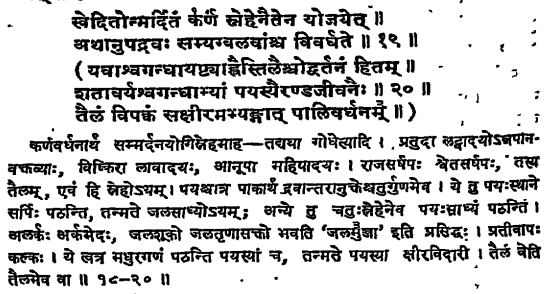
\includegraphics[width=.58\textwidth]{media/yavasva-cakra}\
    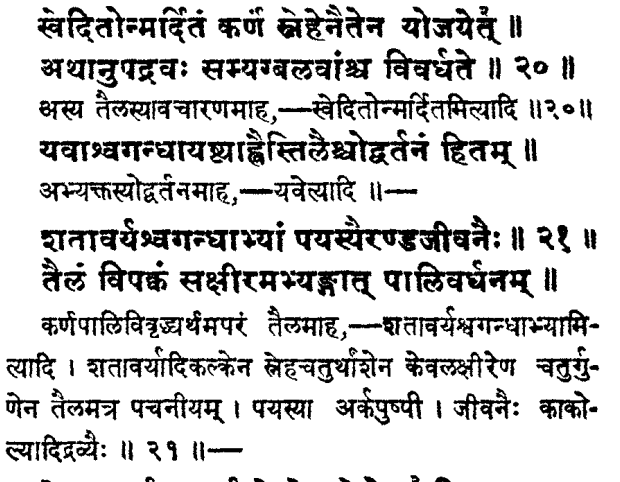
\includegraphics[width=.41\textwidth]{media/yavasva-dalhana}
    \caption{The text as it appears in Cakrapāṇi (left) and Ḍalhaṇa (right)  
    (\cite[130]{acar-1939}, \cite[79]{vulgate}).}
    \label{fig:yavasva}
\end{figure}
citing keywords that show they all
formed part of the main text of the \SS\ that was before
him.\footnote{\Su{1.16.19--23}{79--80}.} However, Cakrapāṇidatta's older
commentary showed no awareness of the first few verses in this group,
Su.1.16.19--21ab.\footcite[130--131]{acar-1939}  Apparently, they were not part of
the text of the \SS\ as he knew it.  In spite of that, the editors printed these
verses in their edition of Cakrapāṇidatta's work as if they were indeed part of
the \SS\ known to to him.\footnote{The editors remarked in a footnote that verses
20--21a were not in the Nepalese manuscript that they consulted \citep[130,
n.\,2]{acar-1939}.}

A similar instance of this occurs in the edition of the \emph{Bhānumatī} at \SS\,1.16.31 
\begin{figure}[t]
    \centering
    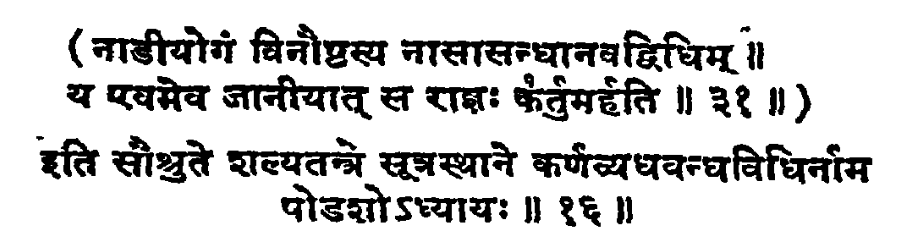
\includegraphics[width=.75\linewidth]{media/nadiyogam}
    \caption{\SS\,1.16.31 in the 1939 printed edition.}
    \label{fig:nadiyogam}
\end{figure}
where the editors of the 1939 printed edition included a verse in parenthesis that was
commented on by Ḍalhaṇa but not by Cakrapāṇidatta (see 
Fig.\,\ref{fig:nadiyogam}).\footnote{The verse begins 
\dev{nāḍīyogaṃ vinauṣthasya}.  It is printed in the vulgate as 
\Su{1.16.32}{81}, with Ḍalhaṇa's commentary.  It is printed in parentheses as 1.16.31 in the 
edition of the Bhānumatī \citep[133]{acar-1939}.} This verse was almost certainly not in the 
text of the \SS\ known to Cakrapāṇidatta. 



The manuscript on which the editor's edition of the \emph{Bhānumatī} was
mainly based,  \MScite{London BL H. T. Colebrooke 908}, does not include the root text of 
the \SS.\footnote{% 
% DW: we don't need to depend on Eggeling because we've now got the MS.
%This observation is based on the
%opening passage \MScite{London IOLR 908}.  
The MS is described in \cite[vol.\,1.5, 928, \#2647]{egge-1887}. 
%of MS 1887-1935 of the \emph{Bhānumatī},
% which is transcribed in Eggling 1896: 928.
%The transcription in this catalogue also shows the commentary without the root text. 
The section on p.\,\pageref{1939edition} below describes the sources that the editors used 
for the 1939 edition.}  Therefore, it requires a detailed reading  of the commentary itself to 
infer what its author, Cakrapāṇidatta, was seeing in the manuscripts of the \SS\ that he had 
before him in the eleventh century.  But, to summarize, there is no evidence that they  
included the verses SS.1.16.19–-21ab and 31 that are printed in \cite{acar-1939} as if they 
were present to Cakrapāṇidatta. 

% got to here

% Ḍalhaṇa 1.16.11–14
%The version of 1.16.11–14 known to Ḍalhaṇa \citep[78]{vulgate} has four verses (\emph{śloka}) at this point that are not in the Nepalese manuscripts. The additional verses iterate the types of joins required for ear flaps that are missing, elongated, thick, wide, etc. All four verses were probably absent in the version of the \emph{Suśrutasaṃhitā} known to Cakrapāṇidatta. He cites the verses separately in his commentary, the \emph{Bhānumatī} \citep[128–129]{acar-1939}, introducing each one as 'some people read' (\emph{ke cit paṭhanti}). However,  in Trikamajī Ācārya's edition of the \emph{Sūtrasthāna} of the \emph{Bhānumatī}, the root text is largely identical to the one commented on by Ḍalhaṇa (\cite{vulgate}), even in instances like this where Cakrapāṇidatta's commentary indicates that he was reading a different version of the \emph{Suśrutasaṃhitā}

% Ḍalhaṇa 1.16.19–20 
%Cakrapāṇidatta \citep[131]{acar-1939} does not comment on these verses, nor verse 15 of the Nepalese version, and so the version of the \emph{Suśrutasaṃhitā} known to him may not have included them.

% Ḍalhaṇa 1.16.32
 %Cakrapāṇidatta \citep[133]{acar-1939} does not comment on this additional verse, which suggests that either he did not know of it or was not inclined to accept it.
 
% Both commentators were aware of a version of the \SS\ that was similar to the Nepalese version % See blog.
\subsubsection{Cakrapāṇidatta and the Nepalese version}
In fact, there is some evidence that the Nepalese version of the \SS\ was more
similar to Cakrapāṇidatta's version than to Ḍalhaṇa's. For example, \SS\,1.16.5 of
the Nepalese version begins with the compound
\dev{doṣasamudayāt}.\footcite[126]{acar-1939} Ḍalhaṇa's version, on the other
hand,  inserted two compounds, \dev{kliṣṭajihmāpraśastasūcīvyadhāt} and
\dev{gāḍhataravartitvāt}, before this.\footnote{\SS\ \Su{1.16.6}{77}.} Cakrapāṇidatta
began his comment on this passage by glossing \dev{doṣasamudayāt}, which
suggests that he was not aware of the compounds that Ḍalhaṇa
saw.\footnote{\SS\,1.16.5 \citep[126–127]{acar-1939}.}

If one looks beyond \SS\,1.16, there are instances where the Nepalese version and
the root text as read by Cakrapāṇidatta have the same reading, but Ḍalhaṇa
mentions it as an alternative that is, “read by others.” For example, \SS\,1.1.28 of
the Nepalese version has \dev{tatrāsmiñ chāstre}, which is also the reading
commented on by Cakrapāṇidatta.\footcite[17]{acar-1939} However, Ḍalhaṇa comments
on \dev{asmiñ chāstre} and states that “others read \dev{tatrāsmiñ
    chāstre}”.\footnote{\SS\ \Su{1.1.22}{5}.} %Also, in his commentary on SS.1.1.8.1,
%Ḍalhaṇa notes the variant reading \dev{ṣaṣṭyā vidhānaiḥ}, which is not in his
% root
%text but evidently was in Cakrapāṇidatta's.\footnote{See \Su{1.1.8.1}{5} and
%SS.1.1.6 \citep[11]{acar-1939} respectively.}
Another example is the reading of \dev{ṣaṣṭyā vidhānaiḥ} in Ḍalhaṇa's commentary
on \Su{1.1.8.1}{3} that is not in his main text but that he ascribes to “some
others.” This reading is likely to be derived  from the expression
\dev{ṣaṣṭyābhidhānaiḥ} in the main text of the Nepalese version, and to have been 
rewritten before Ḍalhaṇa's time because it was hard to understand.\footnote{See
the discussion by \citet[4--5]{birc-2021a}.}

% Ḍalhaṇa was aware of the reading in the Nepalese version because he notes in his commentary on 1.16.6 \citep[77]{vulgate} that some read 'because of the accummulation of humours' rather than 'because of piercing with a painful, crooked and unrecommended needle or because of a wick that is too thick.' 

\subsection{Differences between the Nepalese and Subsequent Versions of SS.1.16}

% The structural differences between the Nepalese and subsequent versions has been 
%discussed by \citet[27–44]{kleb-2021b}, which include the frame story,\footnote{On this 
%topic, also see the more recent \citet{birc-2021}.} the name of the first book 
%(\emph{Ślokasthāna}), the structuring of the text according to chapter and section 
%colophons, 
%and an additional passage in the \emph{Kalpasthāna}. \citet[44–55]{kleb-2021b} also 
%makes 
%general observations on distinct features of the Nepalese version's content and looks 
%specifically at lists of skin lesions arising from urinary disease and vital energies. And in an 
%effort to demonstrate the possibility of greater coherence in the Nepalese version, 
%\citet[101–104]{hari-2011} has compared its classification of snakes with Ḍalhaṇa's 
%version. 

% On the whole, these observations indicate that [...synopsis of general conclusions here, Andrey?...]
%% 1.16 is missing yathovāca bhagavān dhanvantariḥ|

Several differences between the text of the \SS\ as found in its multiple printed
versions and as reconstructed on the basis of the Nepalese MSS have already been
pointed out in previous publications.  \citet[27\,f]{kleb-2021b} listed
differences in the chapter sequence as they affect the overall organization and
structuring themes and elements of the text.  Others have explored variations in
the frame story of the work as a whole.\footcites {wuja-2013} [28-32]{kleb-2021b}
{birc-2021} [2-4]{birc-2021a} \citeauthor{kleb-2021b} highlighted the
interchangeable use of two names of the first book of the text, namely
\emph{Ślokasthāna} and \emph{Sūtrasthāna}. He also discussed another peculiarity
of the Nepalese version, namely the additional verse or prose colophons found at
the end of each book and also at the end of each decade of chapters of the
work.\footcite[32--44]{kleb-2021b}

As the present paper demonstrates, many distinct features pertaining to the actual
content of the Nepalese version continuously come to light as we proceed with our
study of the manuscripts. 

\citet[101–104]{hari-2011} provided an exemplary investigation of textual variants in the 
Nepalese version.  His study looked at the classification of snakes in
\SS\,5.4 and revealed that the Nepalese MSS preserve a text that is internally
more consistent and coherent than the versions of the \SS\ found
in different printed sources.

Klebanov too has contributed some general remarks and examples of substantive differences 
between the Nepalese and vulgate texts 
and detailed two particular case studies.\footcite[44--55]{kleb-2021b} The first
case study dealt with the list of skin lesions associated with urinary disease
(\dev{pramehapiṭakā} in the Nepalese spelling).  Their signs and pathogenesis are
described in the Nidānasthāna and their treatment in the 
\emph{cikitsāsthāna}.\footnote{\Su{2.6}{289--294} and 
\Su{4.12}{454--455} respectively.} 
This list of skin lesions exemplifies a case where the text of the \SS\ transmitted
in the Nepalese MSS is internally more coherent than that commented on by Ḍalhaṇa.
The incoherence of Ḍalhaṇa's version was already identified by an earlier
commentator, Gayadāsa (fl.\,ca.\,1000), 
who
proposed a textual conjecture that corresponds to the reading of the Nepalese
version.\footnote{\MScite{Kathmandu KL 699} was copied a century or more before
    Gayadāsa's time, so its version cannot have been influenced by Gayadāsa's
    innovations or suggestions.} 

The second case study by \citet{kleb-2021b} focussed on the variation in another
list, that of the bodily winds (\dev{prāṇa}, \SS\ 3.4).
This  discussion  too relied upon Gayadāsa's learned remarks. 
He commented on a version of the \SS\ corresponding to the Nepalese MSS 
and reported an alternative reading and its interpretation preferred
by another ancient commentator, Jejjaṭa.  It is precisely 
Jejjaṭa's reading that is known to modern
readers of the \SS\ from the vulgate version of the text. 

The present paper also provides an example of
interpolation.  This is a rare case in which we have a fairly good idea of where
the inserted text came from, namely the medical theory associated with the
\emph{Carakasaṃhitā}.

% got to here. 2022-09-08

On the whole, these observations indicate that many features of the Nepalese version of the 
\SS\ are likely to go back to an early state of the work that was common to other versions of 
the compendium. 
However, other textual features, such as the text-structuring colophons concluding every 
tenth chapter, are likely to have occurred within a local Nepalese transmission of the text, 
and it is improbable that they are attested in the MSS from other regions. 
When evaluating the Nepalese readings historically, it is necessary to keep in mind that there 
is plentiful evidence that Ḍalhaṇa's version of the text also included extremely early 
readings and variants, suggesting that some of the readings accepted by Ḍalhaṇa were 
ancient, if not original.  Each case has to be weighed. 


The following detailed comparison of 1.16 of the Nepalese version with Ḍalhaṇa's 
\emph{Nibandhasaṅgraha} unfolded as the chapter was edited. The differences appear to 
emanate largely from attempts to standardise, simplify or clarify the language of the 
Nepalese version, add and redact information, and introduce changes to recipes and 
treatments. Examples from 1.16 have been provided to demonstrate the general 
observations which, it is hoped, a larger survey of the text will support.

Figure \ref{fig:chapters} reveals the extent to which 1.16 of the Nepalese version
was redacted to create the one known by Ḍalhaṇa. In this particular case,
twenty-seven verses have been added.  Eight of these verses (11--14, 21--22ab,
23cd--24, 32) are well-integrated with the existing material in so far as they
reiterate and elaborate on the content of passages in the Nepalese version. A
block of nineteen verses (26.1--19) at the end of this chapter in Ācārya's edition
of the \emph{Nibandhasaṅgraha} (\cite[80]{vulgate}) was known by Ḍalhaṇa. These
verses cover additional diseases of the ear lobes, with their treatment and
complications. Although Ḍalhaṇa conceded that some read them in this chapter, he
concludes that they were not composed by sages and, therefore, should not be read.
Ācārya probably included these verses because they were in his manuscripts,and
Ḍalhaṇa's comments prompted him to place them in parentheses.\footnote{Ācārya
    (\cite[80]{vulgate}) did not state that these verses were absent in some or all of
    his manuscripts, which he usually did in a footnote if this was the case. A
    broader survey of manuscripts would be helpful for establishing whether these
    verses were part of the transmission of the \SS\ in India. For example, they are
    present in \MScite{Hyderabad Osmania 137-3(b)}.}  Be this as it may, this large
    block of verses is absent in the Nepalese version.  
\begin{figure}[t]
\centering
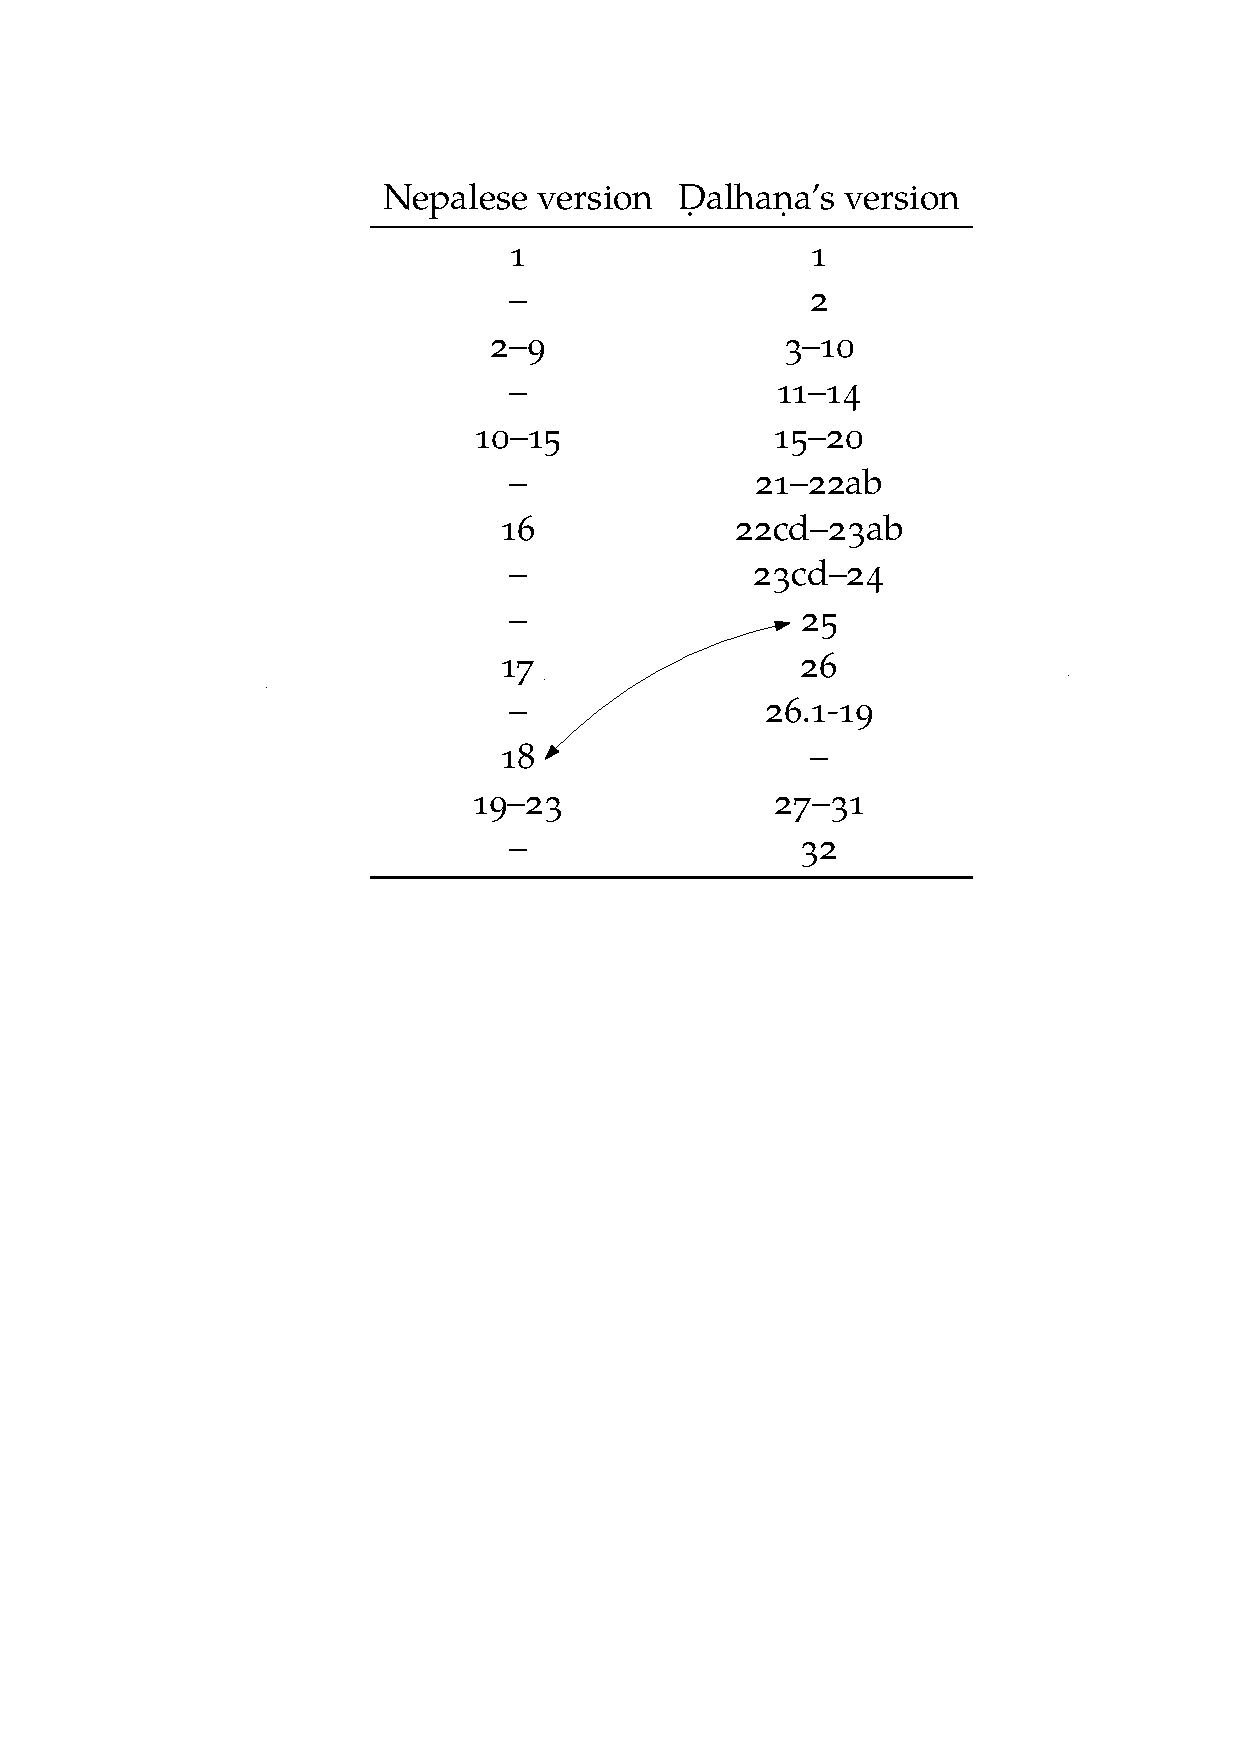
\includegraphics[draft=false,width=.75\textwidth]{table-of-versions.pdf}
\caption{A Comparison of verses in 1.16 of the Nepalese and Ḍalhaṇa's versions.}
\label{fig:chapters}
\end{figure}

In Figure \ref{fig:chapters}, one can also see that verses 17 and 18 of the
Nepalese version were transposed in the redaction of Ḍalhaṇa's version, in which
they are numbered 26 and 25 respectively. Although this only occurs once in 1.16,
such transposing of verses and even their hemistiches is common in the
redaction of other chapters of the \SS.

Apart from the addition of verses, the redacting of the version known to Ḍalhaṇa involved 
many small, yet sometimes significant, changes that are summarised below.\footnote{The 
present study focusses on the commentary of Ḍalhaṇa, but many of the same investigations
    could be made with regard to the surviving parts of the other early commentaries. See the 
    discussion below, p.\,\pageref{ref:dalhana}.}

\subsubsection{Changing Spelling, Sandhi and Syntax}


Later commentators like Ḍalhaṇa often made efforts to standardise, simplify or improve 
the language of the Nepalese version. Such changes include the standardising of 
spelling,\footnote{For example, \dev{pattāṅga} (SS.1.16.21) → \dev{pataṅga} (1.16.29, 
\cite[81]{vulgate}). For more information on this, see the relevant footnote to the 
translation.} sandhi,\footnote{or example, \dev{°hastena ṛju} (SS.1.16.2) → 
\dev{°hastena rju} (1.16.3, \cite[76]{vulgate}).} and verbal forms,\footnote{For example, 
\dev{unnāmayitvā} (SS.1.16.21) → \dev{prānnamya} (1.16.29, \cite[81]{vulgate}); 
\dev{avacūrṇayīta} (SS.1.16.21) → \dev{upaharet} (1.16.29, \cite[81]{vulgate}).} as well 
as interventions to simplify and clarify syntax.\footnote{For example, 
\dev{śoṇitabahutvanivedanāyāṃ cānyadeśaviddham iti jānīyāt | nirupadravatā 
taddeśaviddhaliṅgam |} (SS.1.16.3) → \dev{śoṇitabahutvena vedanayā cānyadeśaviddham 
iti jānīyāt | nirupadravatayā taddeśaviddham iti |} (1.16.4, \cite[76]{vulgate}); 
\dev{āmatailapariṣekeṇopacaret} (SS.1.16.6) → \dev{āmatailena pariṣecayet} (1.16.7, 
\cite[77]{vulgate}); \dev{suparigṛhītaṃ} (SS.1.16.10) → \dev{suparigṛhītaṃ ca kṛtvā} 
(1.16.15, \cite[78]{vulgate}); \dev{anena} (SS.1.16.15) → \dev{snehenaitena} (1.16.20, 
\cite[79]{vulgate}).} These efforts often involved splitting compounds.\footnote{For 
example, 
\dev{yadṛcchāviddhāyāṃ sirāyām} (SS.1.16.4) → \dev{yadṛcchayā viddhāsu sirāsu} 
(1.16.5, \cite[76]{vulgate}); \dev{dhānyāmlakapālacūrṇaṃ} (SS.1.16.10) → 
\dev{dhānyāmlaṃ kapālacūrṇaṃ} (1.16.20, \cite[78]{vulgate}).} In some instances, these 
changes improved the grammar,\footnote{For example, \dev{surāmaṇḍakṣīram} 
(SS.1.16.10) → \dev{surāmaṇḍaṃ kṣīram} (1.16.15, \cite[78]{vulgate}).} or altered the 
meaning.\footnote{For example, \dev{kṣīṇālpamāṃsaḥ} (SS.1.16.12) → \dev{kṣīṇo 
'lpamāṃsaḥ} (1.16.17, \cite[79]{vulgate}).} However, some prefixes of verbal 
forms,\footnote{For example, \dev{samvarddhitaḥ} (SS.1.16.8) → \dev{vivarddhitaḥ} 
(1.16.9, \cite[77]{vulgate}); \dev{niveśya} (SS.1.16.10) → \dev{sanniveśya} (1.16.15, 
\cite[78]{vulgate}); \dev{avabadhya} (SS.1.16.10) → \dev{ca baddhvā} (1.16.15, 
\cite[78]{vulgate}).} case endings,\footnote{For example, \dev{māse} (SS.1.16.2) → 
\dev{māsi} (1.16.3, \cite[76]{vulgate}).} and indeclinables were changed for less apparent 
reasons.\footnote{For example, \dev{api} (SS.1.16.13) → \dev{vā} (1.16.18, 
\cite[79]{vulgate}); \dev{ca} (SS.1.16.16) → \dev{tu} (1.16.23, \cite[79]{vulgate}); 
\dev{tu} (SS.1.16.18) → \dev{ca} (1.16.25, \cite[80]{vulgate}).} There is also a tendency 
to replace uncommon words with generic ones,\footnote{For example, \dev{mrakṣayet} 
(SS.1.16.15) → \dev{yojayet} (1.16.20, \cite[79]{vulgate}); \dev{nahyet} (SS.1.16.21) → 
\dev{baddhvā} (1.16.29, \cite[81]{vulgate}).} add indeclinables,\footnote{For example, 
[absent]  (SS.1.16.6) → \dev{ca} (1.16.7, \cite[77]{vulgate}); [absent] (SS.1.16.10) → 
\dev{tatra} (1.16.15, \cite[78]{vulgate}); [absent]  (SS.1.16.12) → \dev{api} (1.16.17, 
\cite[79]{vulgate}).} omit the verb to be at the end of sentences,\footnote{The words 
\dev{bhavati} or \dev{bhavanti} are omitted four times in Ḍalhaṇa's version (1.16.10 
(twice), 1.16.17 and 1.16.18, \cite[77, 79]{vulgate}).}and introduce verses after a prose 
passage with the phrase \dev{bhavati cātra}.\footnote{For example, [absent] (SS.1.16.11) 
→ \dev{bhavati cātra} (1.16.16, \cite[79]{vulgate}).} 

% Spelling
% 9. nemī → nemi
% 9. yaṣṭī → yaṣṭi
% 9. kākauṣṭhaḥ → kākauṣṭhakaḥ
% 21. pattāṅga → pataṅga *

%Sandhi
% 2 °hastena ṛju  →  °hastena rju (standardise)*

% Standardising and Simplifying Syntax
% 3.  śoṇitabahutvanivedanāyāṃ cānyadeśaviddham iti jānīyāt | nirupadravatā taddeśaviddhaliṅgam || → śoṇitabahutvena vedanayā cānyadeśaviddham iti jānīyāt || nirupadravatayā taddeśaviddham iti ||*
% 6 āmatailapariṣekeṇopacaret → āmatailena pariṣecayet*

% Clarifying syntax
%15 anena → snehenaitena*

% Splitting compounds
% 4. yadṛcchāviddhāyāṃ	sirāyām	 → 	yadṛcchayā viddhāsu	sirāsu (clarifies syntax)*
% 10. surāmaṇḍakṣīram → surāmaṇḍaṃ kṣīram (improves grammar)*
% 10. dhānyāmlakapālacūrṇañ → dhānyāmlaṃ kapālacūrṇañ*
% 12. kṣīṇālpamāṃsaḥ → kṣīṇo 'lpamāṃsaḥ (changes the meaning)*

% Changing verbs and gerunds
% 2. vyadhayet → vidhyete (perhaps, picking up on karnau)
% 6. kurvīta → dadyāt (middle to active) 
% 7. muñcet → kuryāt
% 9. bandhyā bhavanti → sādhyāḥ
% 10. suparigṛhītaṃ → suparigṛhītaṃ ca kṛtvā ( attempt to improve syntax)*
% 10. upapādya → upadhārya
% 10. sandarśya → sandadhyāt | tato (attempt to simplify the sentence)
% 13. chidyeta → chidyate (opt to pres)
% 15. mrakṣayet → yojayet * (replacing less common words with generic ones)
% 21. nahyet → baddhvā*
% 21. unnāmayitvā → prānnamya (standardise)*
%21 avacūrṇayīta → avacūrṇayet (standardise)*

% Omitting bhavati
% Happens a few times; e.g., 1.16.9 (twice), 1.16.12, 1.16.13

% Changing Prefixes
% 8. samvarddhitaḥ → vivarddhitaḥ*
% 10. niveśya → sanniveśya*
% 10. avabadhya → ca baddhvā*
% 15. marditaṃ → unmarditaṃ*
% 21. unnāmayitvā → prānnamya *

% Changing case endings
% 2. māse → māsi (shift from māsa to mās. Can't see a reason)
% 3. śoṇitabahutvanivedanāyāṃ →  śoṇitabahutvena vedanayā (splitting compounds, but locative of circumstance or condition changed to instrumental of reason. latter is clearer, but not much in it)
% 19. viśleṣitāyām atha nāsikāyāṃ → °tāyās tv nāsikāyāḥ

% changing indeclinables
%13 anyathā → ato 'nyathā
% 13 api → vā*
% 15 tataḥ → ataḥ
% 16 ca → tu*
% 18 tu → ca*
% 19 atha → tu
% 23 vai → syāt

% Adding indeclinables
% 10 [absent] → tatra
% 6 [absent] → ca
% 9 [absent] → tu
% 10 [absent] → ca
% 12 [absent] → api
% 14 [absent] → vā

% Omitting indeclinables
% 9 tatra → [absent]
% 9 ca → [absent]

%Adding bhavati cātra before verses.

% Not sure
% 2
% kṛtamaṅgalaṃ svastivācanan → kṛtamaṅgalasvastivācanan (the latter makes better sense, but could have been original, in my opinion, or an attempt to better integrate a gloss that had become part of the text.)
% abhisāntvayamānaḥ → abhisāntvayan (shift from Pres Pass Part to Pres Act Part) % It seems only the latter is correct in the given context. So, it could be just an error in the NV. Emend or Change translation!!! 
% % 10. agropaharaṇīyāt appears to be an error in the NV that needs to be emended.

\subsubsection{Changing Technical Terms}

There is evidence of standardising and altering technical terminology in versions
of the \SS\ subsequent the Nepalese one. Two examples of this in \SS\,1.16 are the
terms for \se{bandha}{joins} and \se{vadhra}{a slice of flesh}. The Nepalese
version uses three terms for \se{bandha, sandhāna, sandhi}{joining} splits in the
ear flaps and the flesh of nose. Redactors of subsequent versions appear to have
tried to standardise this terminology by replacing \dev{sandhāna} and
\dev{sandhi} with \dev{bandha} in prose passages.\footnote{For example,
    \dev{pañcadaśasandhānākṛtayaḥ} (SS.1.16.9) → \dev{pañcadaśabandhākṛtayaḥ}, (cf.\
    \Su{1.16.10}{77}); \dev{daśakarṇasandhivikalpāḥ} (SS.1.16.9) →
    \dev{karṇabandhavikalpāḥ} (cf.\ \Su{1.16.10}{77})} However, the use of the term
    \dev{sandhāna} was retained in verses, perhaps because of the metrical challenges
    of making such a change. Also, the names of joins which incorporate
    \dev{sandhāna} and \dev{sandhi} remained the same.\footnote{These names are
        \dev{nemīsandhānaka}, \dev{kapāṭasandhika}, and \dev{ardhakapāṭasandhika} 
        in
        SS.1.16.9 (cf.\ \Su{1.16.10}{77}).}

The Nepalese version contains the rather obscure term \dev{vadhra} for the slice
of flesh that a surgeon cuts from the cheek in order to construct a new nose
(SS.1.16.20 and 23). Modern dictionaries define \dev{vadhra} as a leathern strap
or a slice of bacon,\footcites[1385]{apte-prac}[917]{moni-sans} the latter of
which is more indicative of its meaning in the Nepalese version. This word was
written out of subsequent versions,\footnote{\dev{vadhram} (SS.1.16.20) →
    \dev{baddham} (SS.1.16.28, \cite[81]{vulgate}) and \dev{tadvadhraśeṣaṃ}
    (SS.1.16.23) → \dev{tad ardhaśeṣaṃ} (SS.1.16.31, \cite[81]{vulgate}).} and it was
    not mentioned as an alternative reading by either Cakrapāṇidatta or Ḍalhaṇa, which
    suggests that its use and meaning may not have been known to them. However,
    \dev{vadhra} was used by the author of the \emph{Aṣṭāṅgahṛdayasaṃhitā} in the
    context of rhinoplasty, so it likely to be the correct reading in the Nepalese
    version.\footnote{\Ah{Utt.18.62}{841}. The word is old, occurring, also in the
        form \dev{vardhra}, from the \emph{Atharvaveda} onwards
        \pvolcite{2}[521--522--277]{mayr-1986}.}

% got to here 

% bandha
% 1. athātaḥ karṇavyadhavidhim vyākhyāsyāmaḥ  → athātaḥ karṇavyadhabandhavidhim adhyāyaṃ (prose)
% sandhāna in all version (verse)
% 9. pañcadaśasandhānākṛtayaḥ (SS.1.16.9) → pañcadaśabandhākṛtayaḥ (SS.1.16.10) (sandhāna is reflected in the name nemisandhānaka, which is in all versions) 
% 9. daśakarṇasandhivikalpāḥ → karṇabandhavikalpāḥ (sandhi is in many of the names, bandha is not)
% 10. (twice) bandha in all versions
% 17 karṇabandha in all versions
% 19 & 23. sandhāna accepted in all versions + 32 in DV. (verse)
% 20. sādhubaddham → sādhubandhaiḥ (verse)
%
% vadhra 
% 20 vadhram → baddham 
% 21 susīvitaṃ → susaṃhitaṃ
% 23 tadvadhraśeṣaṃ → tad ardhaśeṣaṃ

\subsubsection{Augmenting the Text}

Apart from adding whole passages and verses (as seen in Figure \ref{fig:chapters}),
redactors of subsequent versions augmented the text by expanding existing
compounds and inserting new compounds and words. Within the microcosm of 1.16,
adjectives and adverbs were inserted to clarify statements,\footnote{For example,
    \dev{chidre} (\SuComma{1.16.2}{76}) → \dev{chidra ādityakarāvabhāsite}
    (\SuComma{1.16.3}{76}); [absent] (1.16.2) → \dev{śanaiḥ śanaiḥ} (1.16.3); 
    [absent] (SS.1.16.3) → \dev{āśu} (\SuComma{1.16.5}{77}).} and phrases added to
    elaborate on diseases and treatments.\footnote{For example, \dev{dhātryaṅke}
        (SS.1.16.2) → \dev{dhātryaṅke kumāradharāṅke vā} (1.16.3); [absent] (SS.1.16.2) →
        \dev{bālakrīḍanakaiḥ pralobhya} (1.16.3);  [absent] (SS.1.16.3) →
        \dev{picuvartiṃ praveśayet} (1.16.5).} In particular, the characteristics and
        number of symptoms of a disease, as well as their reasons for arising, tend to
        increase in subsequent versions. For example, the Nepalese version (SS.1.16.5)
        said that the wick in a newly pierced ear should be removed because of aggravated
        humours or a culpable piercing whereas the version known to Ḍalhaṇa 
        (\Su{1.16.6}{77}) included two further reasons, namely, because of piercing with
        a painful, crooked and unrecommended needle or because of a wick that is too
        thick. Some of the split ear flaps in Ḍalhaṇa's version have additional
        characteristics,\footnote{For example, \dev{pīṭhopamapālir nirvedhimaḥ}
            (\SuComma{1.16.9}{77}) → \dev{pīṭhopamapālir ubhayataḥ kṣīṇaputrikāśrito
            nirvedhimaḥ} (\SuComma{1.16.10}{77}); \dev{itarālpapāliḥ saṃkṣiptaḥ} 
            (SS.1.16.9)
            → \dev{utsannapālir itarālpapāliḥ saṃkṣiptaḥ} (1.16.10); \dev{tanuviṣamapāliḥ}
            (SS.1.16.9) → \dev{tanuviṣamālpapāliḥ} (1.16.10).} and a list of four symptoms
            associated with incurable joins in the Nepalese version (SS.1.16.19) was increased
            to six in Ḍalhaṇa's version (\Su{1.16.10}{77}). Also, models of
            classifying symptoms were introduced in subsequent versions. For example, the
            Nepalese version (SS.1.16.4) lists the symptoms of mistakenly piercing a duct in
            the ear whereas the version known to Ḍalhaṇa (1.16.5, \cite[76–77]{vulgate})
            classifies these symptoms according to three ducts called \dev{kālikā},
            \dev{marmarikā} and \dev{lohitikā}, which results in some repetition of the
            symptoms mentioned.\footnote{In Ḍalhaṇa's version  (\SuComma{1.16.5}{76–77}), 
            the
                symptoms of \se{jvara}{fever} and \se{vedanā}{pain} are repeated. This 
                repetition
                does not occur in the Nepalese version. It is possible that this classification
                was not in the version of the \SS\ known to Cakrapāṇidatta (1.16.4,
                \cite[126]{acar-1939}) because he mentions that some read classifications of ducts
                at this point in the text and he cites verses from Bhoja on \dev{kālikā},
                \dev{marmarikā} and \dev{lohitikā}, but he does not gloss or comment on the
                passage known to Ḍalhaṇa.}

% Supplementary compounds and phrases for Adding Information
% This is done by expanding compounds, inserting new compounds and adverbs and adding verses and passages.
% 
% 1. karṇavyadhavidhim → karṇavyadhabandhavidhim (foregrounding the term bandha)
% 2
% dhātryaṅke → dhātryaṅke kumāradharāṅke vā (elaborating on treatment)
% upaveśyābhisāntvayamānaḥ → upaveśya bālakrīḍanakaiḥ pralobhyābhisāntvayan (elaborating on treatment)
% chidre → chidra ādityakarāvabhāsite (clarifying technical term)
% [absent] → śanaiḥ śanaiḥ (clarifying treatment)
% [absent] → picuvartiṃ praveśayet (elaborating on treatment)
% 4 
% [absent] →  kālikāmarmarikālohitikāsūpadravā and dividing the adverse affects according to kālikā, marmarikā and lohitikā. Repetition of vedanā and jvara in this process.(discussed in footnote). teṣu yathāsvaṃ pratikurvīt || (adding symptoms, perhaps with a view to managing them more effectively, according to the type of vein pierced).
% 5
% [absent] → kliṣṭajihmāpraśastasūcīvyadhād gāḍhataravartitvād (adding reasons)
% [absent] → yatra saṃrambho vedanā vā bhavati (adding information about the treatment)
%  [absent]  → āśu (clarifies the treatment)
%  [absent] → tāvad yāvat surūḍha iti (until it is well healed - clarifies the treatment)
%9
% pīṭhopamapālir nirvedhimaḥ → pīṭhopamapālir ubhayataḥ kṣīṇaputrikāśrito nirvedhimaḥ (adding characteristics)
% itarālpapāliḥ saṃkṣiptaḥ → utsannapālir itarālpapāliḥ saṃkṣiptaḥ (adding characteristics)
% tanuviṣamapālir → tanuviṣamālpapālir (adding characteristics)
% baddheṣv api dāhapākasrāvaśophayuktā	na siddhim upayānti → tu śophadāharāgapākapiḍakāsrāvayuktā	na siddhim upayānti (adding symptoms)
% 10
% surāmaṇḍodakābhyāṃ → surāmaṇḍoṣṇodakābhyāṃ (adding characteristics of an ingredient)
% 12
% gāḍhapākarāgavān → dāhapākarāgavedanāvān (adding symptoms)

% Additional Verses and Passages (table 1)
% For passages, see subsub on Elaborating on Treatments.
%  [absent] → 16.11–14 (verses)
%  [absent] → 21–22ab, 23cd–24
%  [absent] → 26.1 – 26.19
%  [absent] → 32

\subsubsection{Transposing Words, Verses and Passages}

A close comparison of the Nepalese version with the vulgate reveals changes in the 
order of words, sentences and verses. Examples of such transpositions occur in SS.1.16. In 
most cases, the changes in word order are insignificant and may be result of different 
preferences in syntax or even scribal eye-brain-hand miscommunication.\footnote{For 
example, \dev{aṇusthūla°} (SS.1.16.9) → \dev{sthūlāṇu°} (1.16.10, \cite[77]{vulgate}); 
\dev{tatraite daśakarṇa°} (SS.1.16.9) → \dev{tatra daśaite karṇa°} (1.16.10, 
\cite[77]{vulgate}); \dev{nātigāḍhan nātiśithilaṃ sūtreṇāvabadhya} (SS.1.16.9) → 
\dev{sūtreṇānavagāḍhaman atiśithilaṃ ca baddhvā} (1.16.10, \cite[77]{vulgate}); 
\dev{pūrvan dakṣiṇaṃ kumārasya vāmaṅ kanyāyāḥ | pratanuṃ sūcyā bahalam ārayā } 
(SS.1.16.2) → \dev{pratanukaṃ sūcyā bahalam ārayā | pūrvaṃ dakṣiṇaṃ kumārasya 
vāmaṅ kanyāyāḥ} (1.16.3, \cite[76]{vulgate}).} However, the transposition of verses and 
passages is usually the result of efforts at redacting the text to add new material. A good 
example of this is the transposition of SS.1.16.17 and SS.1.16.18 in the Nepalese version to 
1.16.26 and 1.16.25, respectively, in Ḍalhaṇa's. It seems that this transposition may have 
resulted from the insertion of new verses 1.16.23cd–24 and 1.16.26.1–19 in the latter.

% Words
% 9. aṇusthūla° → sthūlāṇu°
% 9. tatraite daśakarṇa° → tatra daśaite karṇa°
%  10. nātigāḍhan nātiśithilaṃ sūtreṇāvabadhya → sūtreṇānavagāḍhaman atiśithilaṃ ca baddhvā
% Passages
% 2. pūrvan dakṣiṇaṃ kumārasya vāmaṅ kanyāyāḥ | pratanuṃ sūcyā bahalam ārayā || → pratanukaṃ sūcyā bahalam ārayā || pūrvaṃ dakṣiṇaṃ kumārasya vāmaṅ kanyāyāḥ ||
% Verses
%17 and 18 → 26 and 25

%
\subsubsection{Redacting Recipes and Elaborating on Treatments}
Some of the additional text in subsequent versions of the \SS\ introduces new ingredients in 
recipes and different procedures in treatments. In many instances, the new material merely 
clarifies or elaborates on the original but sometimes it changes the recipe or treatment 
significantly. An example of a suppletion that clarifies the text of the Nepalese version can be 
seen in 1.16.3 of Ḍalhaṇa's version (\cite[76]{vulgate}), which contains a statement that the 
physician should insert a wick of cotton after the ear has been pierced.\footnote{For 
example, [absent] (SS.1.16.2) → \dev{picuvartiṃ praveśayet} (1.16.3, \cite[76]{vulgate}).} 
This statement anticipates the instructions in the the Nepalese version (SS.1.16.5–6) on 
removing the wick because of aggravated humours and replacing the wick with a thicker one 
every three days. In this case, the additional statement of Ḍalhaṇa's version elucidates the 
role of the wick in the procedure of piercing the ear. 

A similar clarification occurs in 1.16.18 of Ḍalhaṇa's version (\cite[79]{vulgate}), which reiterates the cure for an ear tainted by a humour that was described in 1.16.7 (= SS.1.16.6). The reiteration is quite apt because it follows a passage  (1.16.17, \cite[79]{vulgate} = SS.1.16.12) that outlines the various symptoms of ear disease arising from each of the three humours. The author of the Nepalese version probably assumed that, after reading SS.1.16.12, the reader would refer back to SS.1.16.6 for the cure of an ear affected by a humour. However, in Ḍalhaṇa's version, the treatment is reiterated at 1.16.18.

In  Ḍalhaṇa's version of 1.16, there are two instances in which ingredients were added to 
recipes of medicines in the Nepalese version. The first is the recipe of an anointment that 
should be applied to a pierced ear that has not healed. In Ḍalhaṇa's version (1.16.7, 
\cite[77]{vulgate}) the recipe was rewritten to include sesame 
seeds.\footnote{\dev{yavamadhukamañjiṣṭhāgandharvahastamūlair madhughṛtapragāḍhair 
ālepayet} (SS.1.16.5) → \dev{madhukairaṇḍamūlamañjiṣṭhāyavatilakalkair 
madhughṛtapragāḍhair ālepayet} (1.16.7, \cite[77]{vulgate}).} A more significant change 
occurs in another recipe for an admixture of an oil that is supposed to be rubbed into a 
healthy ear to enlarge it. Ḍalhaṇa's version (1.16.7, \cite[77]{vulgate}) of the admixture has 
five additional ingredients, namely, \se{apāmārga}{prickly chaff-flower}, 
\se{aśvagandhā}{Withania}, \se{kṣīraśuklā}{giant potato}, \se{madhuravarga}{ the 
`sweet' savour}\footnote{The items which exemplify the `sweet' savour \label{kakolyadi} 
(\dev{madhuravarga}) are enumerated at SS.1.42.11.} and `milk flower' (\dev{payasyā}  
$\rightarrow$ \dev{vidāri}\footnote{Pueraria tuberosa (Willd.) DC. (ADPS 510, IMP 1.792f., 
AVS 4.391; not Dymock 1.424f. See GJM supplement 444, 451, IMP 1.187, but IMP 3.1719 = 
Ipmoea mauritiana, Jacq.). }). It also has \se{vidārigandhā}{beggarweed} instead of 
\se{vidāri}{milk 
flower}.\footnote{\dev{arkālarkabalātibalānantāvidārīmadhukajalaśūkaprativāpan tailam 
pācayitvā } (SS.1.16.14) → 
\dev{arkālarkabalātibalānantāpāmārgāśvagandhāvidārigandhākṣīraśuklājalaśūkamadhuravargapayasyāprativāpaṃ
 tailam vā pācayitvā} (1.16.19, \cite[79]{vulgate}).} This method of redacting a recipe of 
Nepalese version appears to be somewhat typical in so far as most of the ingredients of the 
original were retained and new ones simply added. \q{Perhaps, Dr Madhu could add a 
comment on whether these additional ingredients would change the effects of the treatment 
in any significant way?}


% 2. [absent] → picuvartiṃ praveśayet (adding a cotton wick after piercing the ear of a boy or girl)
% 5. yavamadhukamañjiṣṭhāgandharvahastamūlair	madhughṛtapragāḍhair ālepayet → madhukairaṇḍamūlamañjiṣṭhāyavatilakalkair madhughṛtapragāḍhair ālepayet (adding the ingredient tila)
% 5  [absent] → tāvad yāvat surūḍha iti [...] vidhānaṃ tu pūrvoktam eva || (until it is well healed [... One should pierce it again by] the method taught earlier- clarifies the treatment)
% 13.  [absent] → āmatailena trirātraṃ pariṣecayet trirātrāc ca picuṃ parivartayet | (extending the treatment)
% 14. arkālarkabalātibalānantāvidārīmadhukajalaśūkaprativāpan tailam pācayitvā →	arkālarkabalātibalānantāpāmārgāśvagandhāvidārigandhākṣīraśuklājalaśūkamadhuravargapayasyāprativāpaṃ tailam vā	pācayitvā (adding ingredients to an oil)
% additional apāmārga, aśvagandhā, kṣīra, 

 
    % !TeX root = surgery.tex
\chapter{The Printed Editions}

The careful survey of printed editions of the \SS\ by Meulenbeld lists no fewer than 
44 entries.\footcite[IIB, 311--314]{meul-hist}  These range from the first edition 
by 
Madhusūdana Gupta (\citeyear{gupt-1835}) to editions in the 1970s. The 
number of 
reprints and editions since that time might almost double that number.  
Translations began with Hessler's Latin translation in \citeyear{hess-1855} and 
continue up to the present in scores of publications in many 
languages.\footcites[E.g.,][]{zysk-1984}[IIB, 314--315]{meul-hist}

\section{The vulgate}
\label{vulgate}

The great ayurvedic scholar Yādavaśarman Trivikrama Ācārya produced three
successive editions of the \SS\ with the commentary of Ḍalhaṇa, in 1915, 1931 and
1938.  These editions, especially the last, are generally considered the most
scholarly and reliable editions of the work, and have been constantly reprinted up
to the present day.\footnote{See also the studies of these editions by
    \textcites[\S 1.2]{kleb-2021b}[143--144]{wuja-2013}.}  We refer to the last of
    these editions as “the vulgate.”

The 1915 edition was based on three manuscripts.  The 1931 edition used another
seven manuscripts plus two printed editions.  For his final 1938 edition, Ācārya
used a further three manuscripts.\footnote{The following account is
paraphrased from \citeauthor{vulgate}'s own account of their sources
\citep[22]{vulgate}.}  These sources were described  by Ācārya as follows; we provide 
an overview in Table~\ref{tableofeds}.

\subsection{The sources of the 1915 edition}

\begin{enumerate}
    \item[1] Calcutta, Royal Asiatic Society.  Covers the \emph{sūtra, nidāna, śārīra 
        and 
        kalpa sthāna}s.  
    
    \item [2] Jaipur, Pandit Gaṅgādharabhaṭṭaśarman, lecturer at the Royal 
    Sanskrit University.  Covers the \emph{cikitsāsthāna} and the 
    \emph{uttaratantra}.
    
    \item [3]  Bundi, my great friend the royal physician Paṃ.\ Śrīprasādaśarman  
    Covers the \emph{uttaratantra}.
\end{enumerate}
%
\subsection{The sources of the 1931 edition}

\begin{enumerate}
   \item[1] Vārāṇasī, professor of literature, the great Gaurīnāthapāṭhaka.  With 
    the 
    \emph{Nibandhasaṅgraha}. Covers the \emph{nidānasthāna} and 
    \emph{uttaratantra}.
    
    \item [2]  Ahmedabad.  My friend Sva.\ Vā.\ Vaidya Raṇachoḍalāla 
    Motīlālaśarman.  
    With the \emph{Nibandhasaṅgraha}.  Covers the \emph{śārīrasthāna}.
    
    \item [3] From the personal library of my great friend Sva.\ Vā.\ Vaidya
    Murārajīśarman. Extremely old. No commentary.  Covers the 
    \emph{śārīrasthāna}.
    
    \item [4]  Puṇe, BORI library.  With the \emph{Nibandhasaṅgraha}. Covers the
    \emph{śārīrasthāna}.\footnote{Not one of the three MSS of the
    \emph{śārīrasthāna} described in \cite{shar-vaid}.}
    
    \item [5]  Puṇe, BORI library.  With the \emph{Nibandhasaṅgraha}. Complete.  
    With some damaged folia.
    
    \item [6]  Bombay, Asiatic Society.  Incomplete.\footnote{Possibly 
    \MScite{Mumbai 
    AS B.I.3} or \MScite{Mumbai AS B.D.109} \citep[v.\,1, \# 212 and 
    213]{vela-1930}.  But both these have the \emph{Nibandhasaṅgraha}.  The 
    first 
    covers only the \emph{śārīrasthāna}; the second may be complete, but 
    Velankar calls it 
    only “disorderly.”}
    
    \item [7] Varanasi, the private library of Vaidya Tryambakaśāstrī.  Covers the 
    \emph{cikitsāsthāna}.  The variant readings of this MS were compiled by Prof.\ 
    %    Guruprasādaśāstrī and supplied to Ācārya.
    
    \item [8]  A printed edition together with the commentary 
    \emph{Suśrutasandīpanabhāṣya} by Professor Hārāṇacandra Cakravārtti. 
    Complete work.
    This is the 1910 Calcutta edition numbered “t” by Meulenbeld.\footcites[IB, 
    312]{meul-hist}{bhat-1917}
    
    \item [9] A printed edition of the first 43 chapters of the
    \emph{sūtrasthāna}, printed in Bengali script, with the commentaries
    \emph{Bhānumatī}, \emph{Nibandhasaṅgraha}, edited by Vijayaratnasena and
    Niśikāntasena. This is the 1886 Calcutta edition numbered “g” by 
    Meulenbeld.\footcites[IB,
    311]{meul-hist}{sena-1886}
\end{enumerate}
%

\subsection{The sources of the 1938 edition}
% \coffeestainC{1}{1}{180}{0}{-5 mm}
\begin{enumerate}
    \item [1]  Gwalior, from the library of my great friend Paṃ.\ Rāmeśvaraśāstrin 
    Śukla. 
    Covers the \emph{sūtra, nidāna, śārīra, cikitsā and kalpasthāna}s.
    
    \item[2] Bikaner, from the library of the Royal Palace, supplied by Paṃ.\ 
    Candraśekharaśāstrin. Contains the commentary 
    \emph{Nyāyacandrikāpañjikāvyākhyā} by Gayadāsa.  Covers the 
    \emph{nidānasthāna}.      
    This is almost certainly \MScite{Bikaner Anup 
        4390}.\footnote{See Dominik Wujastyk, “MS Bīkāner AnupLib 4390.” 
    \emph{Pandit}. 
    <\url{http://panditproject.org/entity/108068/manuscript}>.}
    
    \item [3] Kathmandu, located in the private library of the Royal Guru Hemarāja 
    Śarman.  An extremely old palm-leaf manuscript. Readings from this MS were 
    compiled by Paṃ Nityānandaśarman Jośī and sent to Ācārya. Covers from the 
    beginning of the work to the end of the ninth chapter of the 
    \emph{cikitsāsthāna}.  
    
    The siglum for this manuscript in footnotes was \dev{tā} for 
    \dev{tālapatrapustake}. 
\end{enumerate}
\begin{table}
    \centering
      %  \vspace{.5\baselineskip}
        \begin{tabular}{c|ccc|ccccccccc|ccc}
        \toprule
        %        \multicolumn{16}{c}{\emph{Manuscripts (\newmoon) and print 
        %editions 
        %                ($\circ$)}} \\
        \emph{edition}            &\multicolumn{3}{c}{1915}
        &                \multicolumn{9}{c}{1931} 
        &              \multicolumn{3}{c}{1938} \\
        
        \emph{source}         & 1 & 2 & 3 & 1 &2  &3  &4  &5  &6  &7  &8  &9  &1  
        &2 &3 \\
        \midrule
        \emph{sthāna} &&&&&&&&&&&&&&&\\        
        \emph{sū}. &  \newmoon&  &  &
        &  &  &  & \newmoon & ? &  & $\circ$ & 
        $\circ^\dag$ &  
        \newmoon & &\newmoon \\
        
        \emph{ni}. &\newmoon  &  &  &
        \newmoon &  &  &  &  \newmoon&  ?&  & $\circ$ &  &  
        \newmoon&\newmoon & \newmoon\\
        
        \emph{śā}. &  \newmoon&  &  &
        & \newmoon & \newmoon & \newmoon & \newmoon &  ? &  &  
        $\circ$&  &  
        \newmoon& &\newmoon \\
        
        \emph{ci}. &  & \newmoon &  &
        &  &  &  &\newmoon & ? &  \newmoon&$\circ$  &  &
        \newmoon & &\newmoon$^{\dag\dag}$ \\
        
        \emph{ka}.  &\newmoon  &  &  &
        &  &  &  &\newmoon  &  ?&  & $\circ$ &  &  
        \newmoon  & & \\
        
        \emph{utt}.  &  & \newmoon &\newmoon  &
        \newmoon  &  &  &  & \newmoon & ? &  & $\circ$ &  &  
        & & \\
        \bottomrule
    \end{tabular}
    \medskip
    {\small\\
        $^{\dag}$    Covers chapters 1--43 only. \quad
        $^{\dag\dag}$ Covers chapters 1--9 only.
        \par}
    \caption{The sources of Yādavaśarman T. 
        Ācārya's  three editions:\\ manuscript coverage (\newmoon) and print coverage
        ($\circ$). \label{tableofeds}}
\end{table}  
% notes to table 2.
%    \addtocounter{footnote}{-1}
%    \footnotetext{Covers chapters 1--43 only.}
%    \stepcounter{footnote}
%    \footnotetext{Covers chapters 1--9 only.}
%
\subsection{Evaluation}

Estimates show that there are approximately 230 extant manuscript witnesses for
the \emph{Suśrutasaṃhitā}.\footnote{This figure is arrived at by summing the MSS
    mentioned by \tvolcite{39}[373--375]{ncc} and in the \cite{ngmcp}. The real figure
    could be many scores higher.  Cf.\ the overview at
    \cite{wuja-2020}.\label{SSmss}}  Although most of these manuscripts cover only
    parts of the whole work, they amount to approximately twenty times the evidence
    that was used by Ācārya for his vulgate editions.

While the descriptions provided by Ācārya of his source materials seems at
first to be moderately comprehensive, Table~\ref{tableofeds} reveals the
underlying paucity of textual sources for these editions.  At first, it
appears that fifteen manuscripts were consulted.  However, we quickly see that
two of the sources were other people's printed editions, and one of those
covered less than a quarter of the work (no.\,9 of 1931).  That reduces the
manuscript base to 13 witnesses. Ācārya does not appear to have seen two of
the manuscripts at all, having been sent collations prepared for him by others
(7 of 1931 and 3 of 1938).  Thus, Ācārya's final edition was based on the
personal consultation of eleven partial manuscripts.   One of them remains
unidentified (6 of 1931). Only a single manuscript covers the whole of the
\emph{Suśrutasaṃhitā}, no.\,5 of the 1931 edition.  Manuscript 1 of 1938 is
the next most complete, but it omits the \emph{uttaratantra}, which comprises
a third of the work.  Manuscript 1 of the 1915 edition is third in size, but
it still omits both of the longest chapters, and thus offers less than half
the work.  For the rest, the evidence is spotty, with each part of the work
being supported by only between four and eight manuscripts, excluding the
printed editions.

Two sources stand out for their historical importance.  The first is no.\,3 of
1931, which Ācārya calls “extremely old.”  It covered the \emph{śārīrasthāna}
only, and unfortunately we know nothing of the later history of this manuscript.
The second is no.\,3 of 1938, which is one of the important Nepalese manuscripts
being considered in the present project. Ācārya's remarks and references to
Hemarājaśarman's introduction to the \emph{Kāśyapasaṃhitā} allow us to identify
this manuscript as \MScite{Kathmandu NAK
    5-333}.\footnote{\cites[22]{vulgate}[56--57]{hema-1938}. Discussed by \citet[\S
    1.1, 2.3]{kleb-2021b}.  See also \cites[IIB,
    25--41]{meul-hist}[161--169]{wuja-2003}.} The editors of the vulgate,
    \citeauthor{vulgate}, stated that this manuscript covered up to the ninth chapter
    of the \emph{cikitsāsthāna}, but in fact it covers the whole
    work.\footcite[22]{vulgate}  Perhaps the editors only received collations for this
    portion of the manuscript and did not know that it was a witness for the whole
    work.

\section{The 1939 edition}        
\label{1939edition}

In 1939, Yādavaśarman Trivikrama Ācārya and Nandakiśora Śarman co-edited an
edition of the \emph{sūtrasthāna} of the \emph{Suśrutasaṃhitā} that was 
published
by the Swami Laxmi Ram ayurvedic centre in Jaipur, and printed at the famous
Nirṇayasāgara Press in Mumbai (see 
Fig.\,\ref{bhanumati}).\footnote{\cite{acar-1939}.  The description of 
the sources 
below is based on Yādavaśarman T. Ācārya's  remarks in his introduction 
(pp.\,3--4). See also the remarks on this edition by
\citet[7]{kleb-2021a}.  On the Swami Laxmi Ram
centre, see \cite{hofe-2007}} The text was edited on the basis of the following 
sources.

\begin{figure}[p]
    \centering
    \includegraphics[draft=false,height=.9\textheight]{media/Bhanumati-page-11upscaled}
    \caption{A page of the 1939 \emph{Bhānumatī} edition, showing the variant 
        readings in the footnotes.}
    \label{bhanumati}
\end{figure}


\subsection{For the Bhānumatī}

\begin{enumerate}
    \item A printed edition.  Covered the \emph{Bhānumatī} up to chapter Su.sū.40.
    The siglum was \dev{mu} for \dev{mudrita}.\footnote{\cite{sena-1886}.  
    The
    manuscript on which this edition was based is probably in the library of the
    Calcutta Sanskrit College, and described in \cite[v.\,X.1]{sast-1917}, which
    is not available to me.  See also \cite[IB, 495, n.\,57]{meul-hist} for
    mention of this manuscript.  The reference at \cite[217]{rao-sans} to CSCL
    accession number 97 in Bengali script may be this manuscript.}
    
    \item A manuscript in the India Office Library library provided through the
    Bhandarkar Oriental Research Institute in Pune.\footnote{At this time,
    manuscripts from Britain were routinely lent to scholars in India and vice
    versa.} This manuscript covered the \emph{Bhānumatī} up to the end of the
    \emph{sūtrasthāna}.  The siglum was \dev{ha} for
    \dev{hastalikhita}.\footnote{\cite{PP109978}; 
    \MScite{London BL H. T. Colebrooke 908}
    (\href{panditproject.org/entity/109978/manuscript}{PanditProject \#109978},
    consulted on July 03, 2021).}
\end{enumerate}

\subsection{For the Suśrutasaṃhitā}

\begin{enumerate}
    \item A palm leaf manuscript from Hemarājaśarman's personal
    library.\footnote{I.e., \MScite{Kathmandu NAK 5-333}.}  The siglum was
    \dev{tā} for \dev{tāḍapatra}.
    
    \item His own published edition. The siglum was \dev{ḍa} for 
    \dev{ḍalhaṇasaṃmataḥ
        pāṭhaḥ}.\footnote{\cite{vulgate}.  It is noteworthy that Ācārya refers to
    his 1938 edition as representing “the Ḍalhaṇa version.”\label{dalhanaversion}}
    
    \item Hārāṇacandra Cakravarti's published edition with his own
    commentary.\footcite{bhat-1917} The siglum was \dev{hā}.
\end{enumerate}
%
\subsection{Evaluation}

The main innovation of this publication was to present the only surviving part
of the commentary on the \SS\ by the great eleventh-century medical scholar
Cakrapāṇidatta, namely the \emph{Bhānumatī}.\footcite[IA, 374--375 and IB,
495--496]{meul-hist} A secondary purpose was to present the text of the
\emph{sūtrasthāna} as read in \MScite{Kathmandu NAK 5-333}, that had recently
been brought to the editors' attention. In their judgement, the Kathmandu
manuscript presented a text that was closer to what Cakrapāṇidatta had before
him than the text according to Ḍalhaṇa.  In spite of this, the editors largely
reproduced the root text of Ḍalhaṇa's version. This was the first \SS\ edition
in which Ācārya used sigla to identify the sources from which variant readings
were reported, so while it has limitations, it for the first time enables us
to get some idea of origins of his readings at the level of individual words and 
sentences (see Figure~\ref{bhanumati}).

\label{ref:dalhana}Ācārya noted in his introduction that the manuscripts
containing  Ḍalhaṇa's commentary all came together with the root-text of the \SS,
and thus the main \SS\ text reflected the readings chosen by Ḍalhaṇa.  But the
manuscripts of the \emph{Bhānumatī} contained the commentary alone, without the
root-text, and had many explanations based on different readings of the root-text
than those of Ḍalhaṇa.  In many of these cases it was hard to infer what readings
Cakrapāṇidatta had before him. But Ācārya noted that Cakrapāṇidatta had a text
before him that had much in common with the text of the Nepalese
manuscript.\footnote{\cite[3--4]{acar-1939}.  See discussion by
    \citet[7]{kleb-2021a}.}

There is compelling evidence that Cakrapāṇidattas's \emph{Bhānumatī} commentary
once covered the whole text of the \SS.\footcite[IA, 375]{meul-hist}  The loss of
the rest of the work ranks amongst the greatest disasters in Āyurvedic literature.
Remarkably, the whole \emph{Bhānumatī} may still have existed in the early
twentieth century. In 1903, Palmyr Cordier reported being privately informed of a
complete copy of the work in a personal manuscript collection in
Benares.\footcite[332]{cord-1903}
 
    % !TeX root = surgery.tex

\addcontentsline{toc}{section}{Critical Edition of Sūtrasthāna 16}

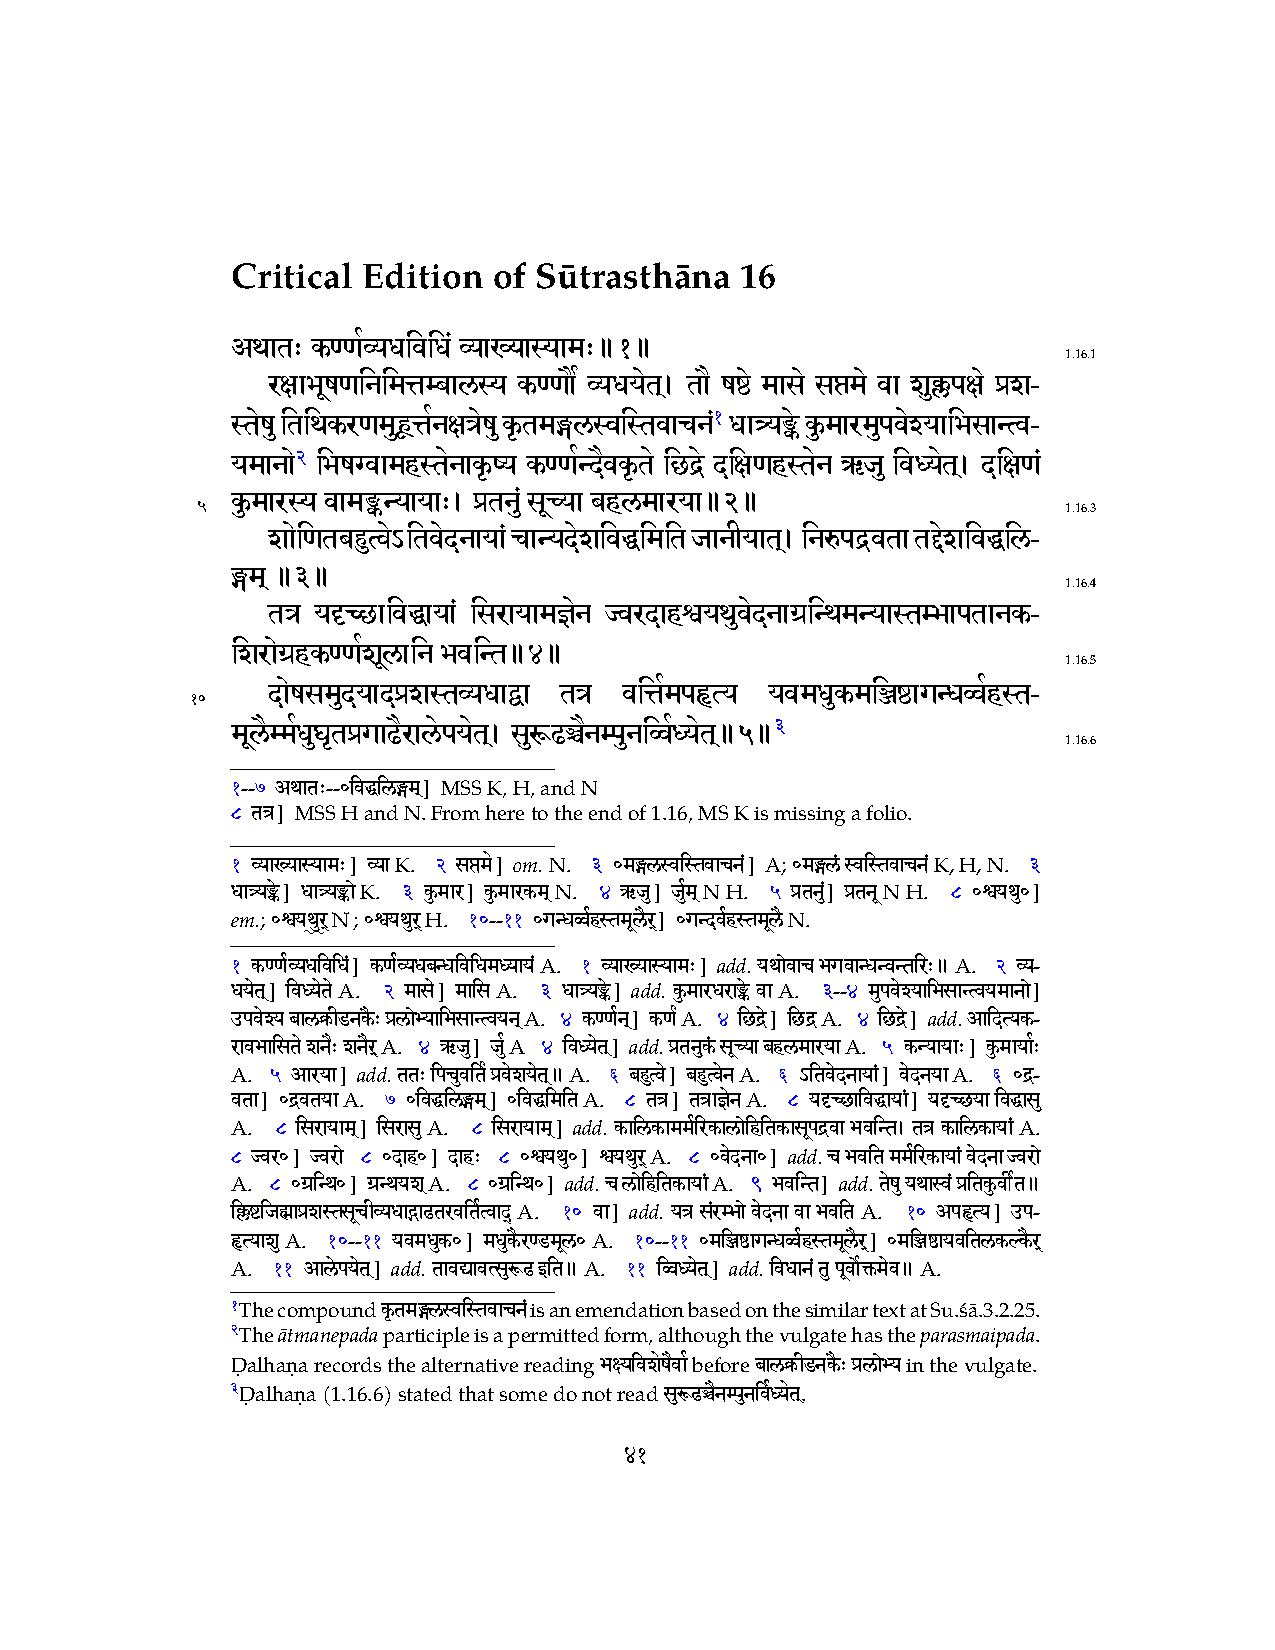
\includepdf[pages=-]{../edition/SS.1.16-critical-edition.pdf}

    % !TeX root = surgery.tex

% turn off the footnotes, for the conference handout
%\renewcommand\footnote[1]{\relax }



%INTRODUCTION
%A. Preliminaries
%1. Aim of the Article
%2. Importance of 1.16 in the History of Āyurveda 
%B. Text
%1. The Nepalese Version
%2. Vulgate
%3. Differences between the Two (as exemplified by 1.16)
%C. Edition 
%1. Manuscripts
%2. Editorial Principles
%EDITION OF 1.16 

  \newcommand{\animal}[4]{#1 (\emph{#2}%\footnote{#3 (#4)})
}
\newcommand{\plant}[4]{#1 (\emph{#2}%\footnote{#3 (#4)})
}
\newcommand\skt[2]{#1 (#2)}


 \section{Translation of Sūtrasthāna 16}
%\subsection{Sūtrasthāna, adhyāya 16}
\renewcommand{\se}[2]{#2 (\dev{#1})} % English with Devanagari in parens
\newcommand{\seEngOnly}[2]{#2} % just the English

\begin{translation}    
  
\item [1] 

Now we shall expound the method for piercing the ear.\footnote{The topic of 
    \se{kaṛnavyadha}{piercing the ear} is not discussed in the \emph{Carakasaṃhitā}
    (\cite[IB, 326, n.\,175]{meul-hist}), but it is mentioned in some texts that
    followed the \emph{Suśrutasaṃhitā}, such as the \emph{Kaśāpyasaṃhitā} \citep[IIA,
    30]{meul-hist}. Also, the instrument for piercing the ear is described in the
    \emph{Aṣṭāṅgahṛdayasaṃhitā} \Ah{1.26.26}{321}. In the versions of the text known
    to Ḍalhaṇa \citep[76]{vulgate} and Cakrapāṇidatta \citep[125]{acar-1939}, the
    heading of this chapter is “the method of piercing and joining the ear”
    (\dev{karṇavyadhabandhavidhi}), instead of the Nepalese version's “the method of
    piercing the ear” (\dev{karṇavyadhavidhi}). The topic of joining the ear
    (\dev{karṇabandha}) is discussed in passages 17--20 of the Nepalese version.
    However, it appears that only subsequent redactors reflected its importance by
    including it in chapter headings.

 The Nepalese version also omits the opening remark on Dhanvantari that appears in
subsequent versions of the text. For a discussion of the frame story in the
Nepalese version, see \cite{birc-2021}. Ḍalhaṇa \citep[76]{vulgate} and
Cakrapāṇidatta \citep[125]{acar-1939} state that only the ears of healthy people
should be pierced, and they quote the lost authority Bhoja to affirm this: “When
piercing the ears of children who are free of disease at these times, their ear
flaps and apertures, as well as limbs, increase” (for the Sanskrit, see
\cite[76]{vulgate}).

Some texts use the adjective \dev{karṇa-vedhanī} rather than \dev{°vyadhanī}.}

\item [2] 

One may pierce a child's ears for the purpose of preserving and decorating. During the
bright fortnight, when the child is in the sixth or seventh month, on renowned
days, half days, hours and constellations, the physician, with a calming presence,
sits the boy, who has received a benediction and the recitation of a
blessing,\footnote{The causative form \dev{vyadhayet} is known in Classical
    Sanskrit \citep[166]{whit-root}.

The compound \dev{kṛtamaṅgalasvastivācanaṃ} “who has received a benediction and
the recitation of a blessing” is an emendation based on the similar text at
\Su{3.2.25}{346}.  Cf.\ also \Su{3.10.8, 24}{388, 390} that have slightly
different formulations.} on the lap of a wet-nurse.\footnote{The versions of
    1.16.3 known to Cakrapāṇidatta \citep[126]{acar-1939} and Ḍalhaṇa
    \citep[76]{vulgate} have the additional compound \dev{kumāradharāṅke} (“on the
    lap of one who holds the child”) after \dev{dhātryaṅke}. The gender of
    \dev{kumāradhara} is made clear by  Ḍalhaṇa's gloss “a man who holds the child.”
    Also, both versions add \dev{bālakrīḍanakaiḥ pralobhya} (“having enticed with
    children's toys”) to indicate that the child should be tempted with toys to stay
    on the assistant's lap. According to Ḍalhaṇa on \Su{1.16.3}{76}, the toys include
    replica elephants, horses, bulls and parrots. Ḍalhaṇa further mentions that others
    read \dev{bhakṣyaviśeṣair vā} (“or by special treats”) before
    \dev{bālakrīḍanakaiḥ}, but we see no trace of these small kindnesses in our
    witnesses.} Then, he should pull the ear with his left hand 
    and pierce straight through with his right hand at a naturally-occurring
    cleft.\footnote{The versions of 1.16.3 of Cakrapāṇidatta \citep[126]{acar-1939}
        and Ḍalhaṇa \citep[76]{vulgate} add that this naturally-occurring cleft is
        illuminated by a ray of sunshine  (\dev{ādityakarāvabhāsite}).

The syntax of this slightly long sentence is unusual in beginning with the dual
object \dev{tau} “the two (ears)” at the start of the sentence, which is remote
from the main verb.  The other singular accusatives referring to the ear being
pierced are governed by absolutives.} For a boy, do the right ear first; for a
girl, do the left one. Use a needle on a thin ear; an \seEngOnly{ārā}{awl} on a thick
one.\footnote{Ḍalhaṇa on 1.16.3 \citep[76]{vulgate} clarifies that the awl is a
    shoe-maker's knife for piercing leather.  He also cites the authority of “the
    notes of Lakṣmaṇa” (\emph{Lakṣmaṇaṭippaṇaka}) on the issue of the thickness of the
    needle. \textit{The Notes of Lakṣmaṇa} is not known from any earlier or
    contemporary sources and was presumably a collection of glosses on the \SS\ that
    was available to Ḍalhaṇa in twelfth-century Bengal. See \citet[IA,
    386]{meul-hist}.}
    
    
\item [3]  
    
One may know that it was pierced in the wrong place if there is excess blood or
too much pain. The absence of side-effects is a sign that it has been pierced in the right
place.\footnote{At this point, \MScite{Kathmandu KL 699} is missing a folio, so
    the rest of this chapter is constructed on the basis of witnesses
    \MScite{Kathmandu NAK 5-333} and \MScite{Kathmandu NAK 1-1079}.}
    
\item [4] 
 
In this context, if an ignorant person randomly pierces a \seEngOnly{sirā}{duct}
there will be fever, burning, \seEngOnly{śvayathu}{swelling}, pain, 
\seEngOnly{granthi}{lumps},
\seEngOnly{manyāstambhā}{paralysis of the nape of the neck}, 
\seEngOnly{apatānaka}{convulsions},
headache or sharp pain in the ear.\footnote{This passage is significantly
    augmented in Cakrapāṇidatta's and Ḍalhaṇa's versions, to outline the specific
    problems caused by piercing three ducts called \dev{kālikā}, \dev{marmikā} and
    \dev{lohitikā} (1.16.4 \citep[126]{acar-1939} and 1.16.5 \citep[77]{vulgate}
    respectively). In fact, the order of the problems mentioned in the Nepalese
    version has been retained in the other versions and divided between each duct.
    Cakrapāṇidatta's commentary on 1.16.4 \citep[126]{acar-1939} cites several verses
    attributed to Bhoja on the problems caused by piercing these three ducts in the
    ear flap: `\dev{lohitikā}, \dev{marmikā} and the black ones are the ducts
    situated in the earflaps.  Listen in due order to the problems that arise when
    they are pierced. Paralysis of the nape of the neck and convulsions, or sharp pain
    arise from piercing \dev{lohitikā}. Pain and lumps are thought to arise from
    piercing \dev{marmikā}. Piercing \dev{kālikā} gives rise to swelling, fever and
    burning.'}
    
\item[5]     
    
Having removed the \se{vartti}{wick} because of the accumulation of
humours or an unsatisfactory piercing at that location,\footnote{In addition to these reasons,
    1.16.6 of Ḍalhaṇa at \Su{1.16.6}{77}, added “because of piercing with a painful,
    crooked and unsatisfactory needle” (\dev{kliṣṭajihmāpraśastasūcīvyadhāt}) and 
    “because of a wick that is too thick” (\dev{gāḍhataravartitvāt}). Ḍalhaṇa was
    aware of the reading in the Nepalese version because in his commentary on
    \Su{1.16.6}{77} he noted that some read “because of the accummulation of humours”
    rather than “because of piercing with a painful, crooked and unsatisfactory needle
    or because of a wick that is too thick.” On the concept of humoral
    \se{samudāya}{accumulation}, see the important analysis by \citet{meul-1992}.} he
    should smear it with barley, liquorice, \seEngOnly{mañjiṣṭhā}{Indian madder},
    and the root of the \seEngOnly{gandharvahasta}{castor oil tree}, thickened with 
    honey and
    ghee. And when it has healed well, he should pierce it again.\footnote{The
        description of the drug is ambigious: the word “root” could be taken with each
        plant, or just with the last.  The vulgate reads just “castor oil root” so we
        assume that is the traditional interpretation.}
    
\item[6] 
    
He should treat the properly-pierced ear by sprinkling it with raw sesame
oil.   After every three days one should make a thicker \seEngOnly{varti}{wick} and
do the very same sprinkling.
%\footnote{The manuscripts support the reading
%    \dev{sthūlatarīṃ} that is either a non-standard form or a scribal error.}
    
\item[7] 
    
Once the ear is free from humours or side-effects, one should put in a light
\se{pravardhanaka}{dilator} in order to enlarge it enough.\footnote{Cakrapāṇidatta
    on 1.16.6 \citep[127]{acar-1939} and Ḍalhaṇa on 1.16.8 \citep[77]{vulgate} pointed
    out that the dilator can be made of wood, such as that of the
    \seEngOnly{apāmarga}{prickly chaff flower}, the \seEngOnly{nimba}{neem tree} 
    and the
    \seEngOnly{kārpāsa}{cotton plant}. Ḍalhaṇa added that it can also be made of
    \seEngOnly{sīsaka}{lead} and should have the shape of the 
    \seEngOnly{dhattūrapuṣpa}{datura
    flower}. The manuscripts have variant readings for \dev{laghupravardhanakam 
    āmuñcet} at this point that include a scribal
    emendation, none of which construe plausibly. It is possible that the unusual
    verb form \dev{ā}+$\surd$\dev{muc} puzzled the scribes and caused 
    the implausible scribal readings and emendations.} 
    
\item[8]
    
\begin{sloka}
A person's ear enlarged in this way can split in two, either as a result of the 
humours\footnote{Ḍalhaṇa on 1.16.9  \citep[77]{vulgate} notes that the word \dev{doṣa} 
here can refer to either a humour, such as \seEngOnly{vāta}{wind}, as we have 
understood it, or a 
disease generated from a humour.} or a blow.\\ Listen to me about the 
\seEngOnly{sandhāna}{ways of joining} 
it can have. 
    \end{sloka}
    
\item[9]
    
Here, there are, in brief, fifteen ways of mending the ear flap.\footnote{The Nepalese version 
uses the word \dev{sandhāna} to refer to joining a split in an ear flap, which is consistent 
with the terminology in the verse cited above (8). However, 1.16.10 of Ḍalhaṇa's version 
\citep[77]{vulgate} uses the term \dev{bandha} here and at the very beginning of the 
chapter (i.e., 1.16.1) to introduce the topic of repairing the ear.}  They are as follows:
    \se{nemīsandhānaka}{Rim-join}, \se{utpalabhedyaka}{Lotus-splittable}, 
    \se{vallūraka}{Dried Flesh}, \se{āsaṅgima}{Fastening}, \se{gaṇḍakarṇa}{Cheek-ear}, 
    \se{āhārya}{Take away}, \se{nirvedhima}{Ready-Split}, \se{vyāyojima}{Multi-joins}, 
    \se{kapāṭasandhika}{Door-hinge}, \se{ardhakapāṭasandhika}{Half door-hinge}, 
    \se{saṃkṣipta}{Compressed}, \se{hīnakarṇa}{Reduced-ear},
    \se{vallīkarṇa}{Creeper-ear}, \se{yaṣṭīkarṇa}{Stick-ear}, and \se{kākauṣṭha}{Crow's lip}.\footnote{For an artist's impression of these different kinds of joins in the ear flap, see \cite[290]{majn-1975} (reproduced as Figure 3.2 in \cite[154]{wuja-2003}).}
    
    In this context, among these, 

    \begin{description}
        
\item[\mdseries``Rim-join'':]
        both flaps are wide, long, and equal.
        
\item[\mdseries``Lotus-splittable'':]
        both flaps are round, long, and equal.
        
\item[\mdseries``Dried flesh'':]
        both flaps are short, round, and equal.
        
\item[\mdseries``Fastening'':]
        one flap is longer on the inside.
        
\item[\mdseries``Cheek-ear'':]
        one flap is longer on the outside.\footnote{For an artist's impression of this join, see \cite[291]{majn-1975} (reproduced as Figure 3.3 in \cites[155]{wuja-2003}).}
        
\item[\mdseries``Take-away'':]
        the flaps are missing, in fact, on both sides.
        
\item[\mdseries``Ready-split'':]
        the flaps are like a \se{pīṭha}{dais}.
        
\item[\mdseries``Multi-joins'':]
        one flap is small, the other thick, one flap is equal, the other unequal.
        
\item[\mdseries``Door-hinge'':]
        the flap on the inside is long, the other is small.
        
\item[\mdseries``Half door-hinge'':]
        the flap on the outside is long, the other is small.
    \end{description}

`These ten options for \seEngOnly{sandhi}{joins} of the ear should be
bound.  They can mostly be explained as resembling their
names.\footnote{Cakrapāṇidatta on 1.16.9–13 \citep[128–129]{acar-1939} and Ḍalhaṇa
    on \Su{1.16.10}{77–78} provide examples of how the names of these joins describe
    their shapes. For example, the \se{nemīsandhānaka}{rim-join} is similar to the
    join of the \se{cakradhārā}{rim of a wheel}.}  The five from
    \se{saṃkṣipta}{compressed} on are incurable.\footnote{Ḍalhaṇa on
        \Su{1.16.10}{77–78} mentions that some do not read the statement that only five
        are incurable, and they understand the causes of unsuccessful joins given below
        (i.e., heat, inflammation, suppuration and swelling) as also pertaining to the
        first ten when they do heal.}  Among these, “Compressed” has a dry ear canal and
        the other flap is small.   “Reduced ear” has flaps that have no base and have
        wasted flesh on their edges. “Creeper-ear” has flaps that are thin and uneven.
        “Stick-ear” has \seEngOnly{granthita}{lumpy} flesh and the flaps are stretched thin 
        and
        have \seEngOnly{stabdha}{stiff} \seEngOnly{sirā}{ducts}.  “Crow-lip” has a flap 
        without flesh
        with \seEngOnly{saṃkṣipta}{compressed} tips and little blood. Even when they are 
        bound
        up, they do not heal because they are hot, inflamed, 
        \seEngOnly{srāva}{suppurating}, or
        swollen.\footnote{The version of 1.16.11–13 known to Ḍalhaṇa \citep[78]{vulgate}
            has four verses (\dev{śloka}) at this point that are not in the Nepalese
            manuscripts. The additional verses iterate the types of joins required for ear
            flaps that are missing, elongated, thick, wide, etc. All four verses were probably
            absent in the version of the \emph{Suśrutasaṃhitā} known to Cakrapāṇidatta. He
            cites the verses separately in his commentary, the \emph{Bhānumatī}
            \citep[128–129]{acar-1939}, introducing each one as 'some people read' (\dev{ke
            cit paṭhanti}). However,  in Trikamajī Ācārya's edition of the \emph{Sūtrasthāna}
            of the \emph{Bhānumatī}, the root text is largely identical to the one commented
            on by Ḍalhaṇa (\cite{vulgate}), even in instances like this where Cakrapāṇidatta's
            commentary indicates that he was reading a different version of the
            \emph{Suśrutasaṃhitā}. See further the discussion on p.\,\pageref{skinflap}
            above.} 
            %            \q{The vulgate verses missing in the Nepalese version here
            %                are worth noting because they are explicit about a skin-flap
            % graft remaining
            %                connected to the site of removal.}
            %
            \item[10]
    
    % 15
A person wishing to perform a join of any of these should therefore have supplies
specially prepared according to the recommendations of the “Preparatory Supplies”
chapter.\footnote{\emph{Suśrutasaṃhitā} \Su{1.5}{18–23}, probably verse 6
    especially that lists the equipment and medications that a surgeon should have
    ready.}  And in this regard, he should particularly gather\footnote{The reading in
        the Nepalese manuscripts of \dev{viśeṣataś cāgropaharaṇīyāt} has been emended to
        \dev{viśeṣataś cātropaharet} to make sense of the list of ingredients, which is
        in the accusative case. Also, the repetition of \dev{agropaharaṇīyāt} in the
        Nepalese version suggests that its second occurrence, which does not make good
        sense here, is a dittographic error.} \se{surāmaṇḍa}{decanted liquor}, milk,
        water, \seEngOnly{dhānyāmla}{fermented rice-water}, and 
        \se{kapālacūrṇa}{powdered
            earthenware crockery}.\footnote{The term \dev{kapālacūrṇa} is unusual. Ḍalhaṇa
            \citep[79]{vulgate} defines it as the powder of fragments of fresh earthen pots
            and Cakrapāṇidatta \citep[129]{acar-1939} as the powder of earthenware vessels.}
    
Next, having made the woman or man tie up the ends of their hair, eat lightly and
be firmly held by qualified attendants, the physician considers the
\seEngOnly{bandha}{joins} and then applies them by means of 
\seEngOnly{chedya}{cutting},
\seEngOnly{bhedya}{splitting}, \seEngOnly{lekhya}{scarification}, or
\seEngOnly{vyadhana}{piercing}.\footnote{There are syntactic difficulties in this
    sentence.  We have %    It appears that a verb has
    %dropped out of this sentence in the Nepalese version because each word of the
    %sentence is in the accusative case with no apparent verb. Therefore, we have
    adopted the reading in Ḍalhaṇa's version \citep[78]{vulgate}, which has
    \dev{ca kṛtvā} following \dev{suparigṛhītaṃ}. It is likely that a verb, such
    as \dev{kṛtvā}, dropped out of the Nepalese transmission.}  Next, he should
    examine the blood of the ear to know whether it is \seEngOnly{duṣṭa}{tainted} or not.
    If it is tainted by wind, the ear should be bathed with
    \seEngOnly{dhānyāmla}{fermented rice-water} and water; if tainted by choler, then
    cold water and milk should be used; if tainted by phlegm, then
    \seEngOnly{surāmaṇḍa}{decanted liquor} and water should be used, and then he 
    should
    scarify it again.
       
After arranging the join in the ear so that it is neither proud, depressed, nor
uneven, and observing that the blood has stopped, one should anoint it with
honey and ghee, bandage each ear with \seEngOnly{picu}{cotton} and 
\se{plota}{gauze}, and
bind it up with a thread, neither too tightly nor too loosely.  Then, the
physician should sprinkle earthenware powder on it and  provide
\se{ācārika}{medical advice}. And he should supplement with food as taught in  the
“Two Wound” chapter.\footnote{\emph{Suśrutasaṃhitā} 4.1 \citep[396–408]{vulgate}.}
    
\item[11]
\begin{sloka}
        One should avoid rubbing, sleeping during the day, exercise, overeating,\\
        sex, getting hot by a fire, or the effort of speaking.
    \end{sloka}

\item[12]
    
    % 17
One should not make a join when the blood is too pure, too copious, or too
thin.\footnote{1.16.17 of Ḍalhaṇa's version \citep[79]{vulgate} reads “impure” for
    the Nepalese “too pure,” which would appear to make better medical sense. Emending
    the text to \dev{nāśuddha-} for \dev{nātiśuddha-} in the Nepalese recension would
    yield the same meaning as the Ḍalhaṇa's version.} For when the ear is tainted by
    wind, then it is \seEngOnly{raktabaddha}{obstructed by blood}, unhealed and will
    peel. When tainted with choler, is becomes \se{gāḍha}{pinched},
    \seEngOnly{pāka}{septic} and red.  When tainted by phlegm, it will be
    \seEngOnly{stabdha}{stiff} and itchy.  It has excessively copious
    \seEngOnly{srāva}{suppuration} and is \seEngOnly{śopha}{swollen}.  It has a small
    amount of \se{kṣīṇa}{wasted} flesh and it will not grow.\footnote{In his edition
        of \emph{Suśrutasaṃhitā}, Ācārya \citep[79 n. 1]{vulgate} includes in parentheses
        the following treatment for these conditions, which according to a footnote is not
        found in the palm-leaf manuscript he used: 'One should sprinkle it with raw sesame
        oil for three days and one should renew the cotton bandage after three days'
        (\dev{āmatailena trirātraṃ pariṣecayettrirātrācca picuṃ parivartayet}).}
    
\item[13] When the ear is properly healed and there are no complications,  one may
very gradually start to expand it.  Otherwise, it may be \se{saṃrambha}{inflamed},
burning, septic or painful.  It may even split open again.
    
\item [14]
    
Now, massage for the healthy ear, in order to enlarge it.
     
One should gather as much as one can the following: a \seEngOnly{godhā}{monitor 
lizard},
%{godhā}{Varanus bengalensis, Schneider}{Daniel 1983:58},
\seEngOnly{pratuda}{scavenging} and \seEngOnly{viṣkira}{seed-eating} birds, and
\seEngOnly{ānūpaudaka}{creatures that live in marshes or water},\footnote{For such
    classifications, see the analyses by \citet{zimm-1999} and \citet{smit-1994}.} fat, 
    marrow, milk,
    and sesame oil, and white mustard oil.\footnote{Ḍalhaṇa's version of \Su{1.16.19}{79}
        includes \seEngOnly{sarpis}{ghee}. However, Ḍalhaṇa's remarks on this passage 
        and
        Cakrapāṇidatta's on 1.16.18 \citep[130]{acar-1939} indicate that they knew a
        version of this recipe, perhaps similar to the Nepalese one, that did not include
        ghee. Ḍalhaṇa also noted that others simply read four oils, beginning with fat
        and without milk, whereas Cakrapāṇidatta said that some say it is made with four
        oils and milk.}\q{think more about the compound structure here?} Then cook the oil
        with an \seEngOnly{prativāpa}{admixture} of the following: \se{arka}{purple 
        calotropis},
        %{Calotropis gigantea, (L.) R. Br.}{ADPS 52, AVS
        % 1.341, NK \#427, Potter 57, ID 306},
        \se{alarka}{white calotropis}, %{Calotropis procera, (Ait.) R. Br.}{NK
        % \#428,
        % GIMP 46b, ID 306},
        \se{balā}{country mallow}, %{Sida cordifolia, L.}{ADPS 71, NK \#2297},
        \se{atibalā}{`strong Indian mallow'}, %{Abutilon indicum, (L.) Sweet; Sida
        % rhombifolia, L.?}{NK \#11, IGP ,4 1080; NK \#2300},
        %\plant{Indian sarsaparilla}{anantā}{Hemidesmus indicus, (L.) R.
        %  Br. \textnormal{and} Cryptolepis buchanani, Roemer \&
        %  Schultes}{ADPS 434, AVS 3.141, NK \#1210},
        %the \skt{Indian sarsaparillas}{sārive}
        \se{anantā}{country sarsaparilla}, %{Hemidesmus indicus, (L.) R. Br.}{ADPS
        % 434,AVS 3.141--5, NK \#1210}
        %and
        %\plant{black creeper}{pālindī}{Ichnocarpus frutescens, (L.)
        %    R.Br. \textnormal{or} Cryptolepis buchanani, Roemer \&
        %    Schultes}{AVS 3.141, 3.145, 3.203, NK \#1283, \#1210, ADPS
        %    434}),
        %
        %%\plant{prickly chaff-flower}{apāmārga}{Achyranthes aspera,
        %%    L.}{GJM 524f., IMP 1.39, ADPS 44f., IMP 3.2066f., Dymock 3.135},
        %\plant{Withania}{aśvagandhā}{Withania somnifera (L.) Dunal}{IMP
        %    5.409f., Dymock 2.566f., Chevallier 150.},
        \se{vidāri}{beggarweed}, %{Desmodium gangeticum (L.) DC}{Dymock 1.428, GJM
        % 602, cf.\ NK \#1192; ADPS 382, 414 and IMP 2.319, 4.366 are confusing},
        %\plant{giant potato}{kṣīraśukla  $\rightarrow$ kṣīravidārī}{Ipmoea
        % mauritiana,
        %    Jacq.}{ADPS 510, AVS 3.222, IMP 3.1717ff.},
        \se{madhuka}{liquorice} and hornwort (\dev{jalaśūka} $\rightarrow$
        \dev{jalanīlikā}\footnote{Ceratophyllum demersum, L. %(IMP 2371, AVS
            % 2.56,
            % IGP 232).
            This name is not certain. In fact, Ḍalhaṇa on 1.16.19
            \citep[79]{vulgate} notes that some people interpret it as a
            poisonous, hairy, air-breathing, underwater creature.}).%
            %items having the `sweet' savour (\dev{madhuravarga}\footnote{The
            %items which exemplify the `sweet' savour \label{kakolyadi}
            % (\dev{madhuravarga}) are enumerated at SS.1.42.11.})
            %and `milk
            %flower'(\dev{payasyā}  $\rightarrow$ \dev{vidārī}\footnote{Pueraria
            %tuberosa (Willd.) DC.
            %(ADPS
            %    510, IMP 1.792f., AVS 4.391; not Dymock 1.424f. See GJM
            % supplement 444,
            %    451, IMP 1.187, but IMP 3.1719 = Ipmoea mauritiana, Jacq.).
            \footnote{The version of 1.16.19 known to Ḍalhaṇa \citep[79]{vulgate}
                adds several ingredients to this admixture, including \dev{apāmārga,
                aśvagandhā, kṣīraśuklā, madhuravarga} and \dev{payasyā}. Also, it has
                \dev{vidārigandhā} instead of \dev{vidāri}. When commenting on
                1.16.19, Ḍalhaṇa \citep[79]{vulgate} notes that some do not read
                \dev{madhuravarga} and \dev{payasyā}. Therefore, there were probably
                other versions of this recipe with fewer ingredients, as seen in the
                Nepalese version.} %
                This should then be deposited in a well-protected spot.
    
\item[15]% 20
    \begin{sloka}
The wise man who has been sweated should rub the \seEngOnly{mardita}{massaged} 
ear with
it.\\ Then it will be free of complications, and will enlarge properly and be
strong.\footnote{For these aims (i.e., healing and enlarging the ear), the text
    known to Ḍalhaṇa \citep[79]{vulgate} has an additional verse and a half describing
    an \seEngOnly{udvartana}{ointment for rubbing the ear} and 
    \seEngOnly{taila}{sesame oil} cooked
    with various medicines for massage. Cakrapāṇidatta \citep[131]{acar-1939} does not
    comment on these verses, nor verse 15 of the Nepalese version, and so the version
    of the \emph{Suśrutasaṃhitā} known to him may not have included them.}
    \end{sloka}
    
\item[16]
    % 22cd-23
        \begin{sloka}
Ears which do not enlarge even when sweated and oiled,  should be scarified  at the
\seEngOnly{apāṅga}{edge of the hole}, but not outside it.\footnote{Dalhaṇa's version of
    \Su{1.16.23}{79--80} adds another hemistich that states more explicitly that the
    scarification should not be done on the outside of hole as it will cause
    derangement.}
        \end{sloka}
    
\item[17]
          \begin{sloka}
    In this tradition, experts know countless repairs to ears.  So a 
    physician who is \seEngOnly{suniviṣṭa}{very intent} on working in this way 
    \seEngOnly{yojayed}{may repair} them.\footnote{After verse 17, the 1938 edition of 
    Ācārya 
    \citep[80]{vulgate} has in parentheses nineteen verses on diseases of the ear lobes, 
    treatments and complications. It is possible that these verses were in some of the 
    witnesses used by Ācārya to construct the text as they occur in other manuscripts, such as  
    MS Hyderabad Osmania 137-3 (b). However, Cakrapāṇidatta \citep[132]{acar-1939} and 
    Ḍalhaṇa \citep[80]{vulgate} state that some read about the diseases of the ear lobes in 
    this chapter whereas others read about them in the chapter on 
    \se{miśrakacikitsa}{various treatments} (SS 5.25), which does indeed begin with a 
    discussion of the disease \dev{paripoṭa}.  Ḍalhaṇa goes on to say that some believe that 
    these verses were not composed by sages and, therefore, do not read them.}
        \end{sloka}
    
\item[18]
    % 25
           \begin{sloka}
    If an ear has grown hair, has a nice hole, a firm join, and is strong and
    even, well-healed, and free from pain, then one can enlarge it slowly.\footnote{The order of verses 17 and 18 are reversed in Ḍalhaṇa's version \citep[80]{vulgate}.}
        \end{sloka}
    
\item[19]
    
    %28, 29.
   \begin{sloka}
        Now I shall describe the proper method of making a repair when a nose is severed.
    First, take from the trees a leaf the same size as the man's nose and hang it
    on him. 
   \end{sloka}
    
\item[20] 

\begin{sloka}
    Next, having cut a \se{vadhra}{slice of flesh},\footnote{The
    version of 1.16.28b known to Ḍalhaṇa \citep[81]{vulgate} reads “\se{baddham}{bound, 
    connected}” instead of “\se{vadhra}{slice of flesh}.”
    This is a critical variant from the surgical point of view.  If the slice remains
    connected, it will have a continuing blood supply.  This is one of the effective 
    techniques that so astonished surgeons witnessing a similar operation in Pune in
    the eighteenth century \citep[see][67--70]{wuja-2003}.} with the same
    measurements, off the cheek, the end of the nose is then scarified.\footnote{Or 1.16.20 
    could be mean, 
    `\ldots\ off the cheek, it is fixed to the end of the nose, which has been
    scarified.' Unfortunately, the Sanskrit of the Nepalese version is not unambiguous on the
    important point of whether or not the flap of grafted skin remains connected
    to its original site on the cheek. However, Ḍalhaṇa \citep[81]{vulgate} clarifies the 
    meaning of the vulgate here by stating that one should supply the word 'flesh' when 
    reading 'connected,' thus indicating that he understood the flesh to be connected to the 
    face.} % 
%
Then the \seEngOnly{apramatta}{undistracted} physician, 
    should quickly put it back together so that it is 
    \seEngOnly{sādhubaddha}{well joined}.
    \label{well-joined}
\end{sloka}  


\item[21] 
    % 30.
\begin{sloka}
Having carefully observed that it has been sewn up properly, he should then fasten
it along with two tubes.\footnote{Ḍalhaṇa noted that the two tubes should be made
    of \seEngOnly{nala}{reed} or the \seEngOnly{eraṇḍapatranāla}{stalk of the leaf of 
    castor oil
    plant} (on \Su{1.16.21}{81}). They should not be made of lead or betel nut because
    the weight will cause them to slip down.} Having caused it to be
    raised,\footnote{The Sanskrit term \dev{unnāmayitvā} in 1.16.21 is non-Pāṇinian.}
        the powder of \seEngOnly{pattāṅga}{sappanwood},\footnote{Caesalpinia sappan, 
        L. %(AVS
            % 1.323, IMP 2.847f.).
            For \dev{pattāṅga} there are manuscript variants \dev{pattrāṅga}
            (\MScite{Kathmandu NAK 5-333}) and \dev{pattaṅga} (\MScite{Kathmandu NAK
            1-1079}).  Also, \MScite{Kathmandu KL 699} (f.\,14r:1) has \dev{pattrāṅga} in
            a verse in 1.14 (cf.\ \Su{1.14.36}{66}). The text known to Ḍalhaṇa  has
            \dev{pataṅga} (\Su{1.16.29}{81}) and this term is propagated in modern
            dictionaries.} %\se{yaṣṭīmadhuka}
            {liquorice} %{Glycyrrhiza glabra, L.}{AVS 3.84, NK \#1136},
            and Indian barberry.\footnote{Berberis aristata, DC. % (Dymock 1.65, NK 
                % \#685, GJM 562, IGP 141).
                Ḍalhaṇa understands it as \se{rasāñjana}{elixir salve}
                (\cite[81]{vulgate}).}\q{añjana} should be sprinkled on it.

\end{sloka}    
\item[22] 
\begin{sloka}
 The wound should be covered properly with \seEngOnly{picu}{cotton} and should be
moistened repeatedly with sesame oil.  Ghee should be given to the man to drink. 
His digestion being complete, he should be oiled and purged in accordance with
the instructions specific to him.\footnote{The expression \dev{svayathopadeśa}
    is ungrammatical but supported in all available witnesses.}
\end{sloka}
    
\item[23] %32.
\begin{sloka}
And once healed and really come together, what is left of that \se{vadhra}{slice
    of flesh} should then be trimmed.\footnote{The vulgate transmission has lost the
    word \dev{vadhra} and replaced it with \dev{ardha} “half,” which makes little
    sense in this surgical  context.} If it is \seEngOnly{hīna}{reduced}, however, one 
    should
    make an effort to stretch it, and one should make its overgrown flesh
    smooth.\footnote{Ḍalhaṇa  accepted a verse following this, \Su{1.16.32}{81}, which
        points out that the procedure for joining the nose is similar to that of joining
        the lips without fusing the ducts. He noted that earlier teachers did not think
        this statement on the nose and lips was made by sages, but he included it because
        it was accepted by Jejjaṭa, Gayadāsa and others, although they did not comment on
        it because it was easy to understand. Cakrapāṇidatta also did not comment on this
        additional verse \citep[133]{acar-1939}.}

\end{sloka}    
    
\end{translation}    
 
    %\section{Nidānasthāna}

% now the end matter

%Cf.\ \cite{adri-engl}.
\nocite{*} % include everything from the bib file in the bibliography


\printbiblist[heading=biblistintoc,notkeyword=botanical]{shorthand} % the 
%Abbreviations (shorthands)

\indexprologue{\emph{\footnotesize (The numbers after the first comma refer to 
pages.)}} 
    
\printindex[manuscripts]

\printbibliography
[notkeyword=edition,
notkeyword=shorthand,
heading=bibintoc]

\printbiblist[title=Botanical sourcebooks,
    heading=biblistintoc,
    keyword=botanical]{shorthand} 
    
{\footnotesize
    
%    \printindex[lexical]
    
    % glossary of plants \gls{klītaka}
    \renewcommand{\glossaryname}{Glossary and Index of Medical Substances}
    \printunsrtglossaries % plant names.  iterate over all defined entries 
    
    \par}




 

%    \section*{Appendix}
\subsection{On digital critical editions}

\begin{itemize}
    \item \fullcite{pric-2013}. \\ A survey of the field in 2013, with a focus on
    the presentation of electronic texts rather than on critical editing as such.
    
    \item \fullcite{mour-2015}. \\ Useful discussion about the \emph{apparatus criticus}
    in general, and an evaluation of the plus and minus points of positive and
    negative apparatuses. 
    
    \item \fullcite{burg-2016}. \\ Discussion of a software tool, including the
    handling of positive and negative apparatus.  Makes the assumption that online
    displays are notational variants only.
    
    \item \fullcite{burg-2017}.  \\ Discussion of how to express various kinds of apparatus in 
    TEI.
    
    \item \fullcite{baus-2015b}. \\ A huge book that disappointingly says nothing at all about 
    Sanskrit manuscripts.  Nevertheless there are many interesting case studies and remarks 
    applicable to the Indian manuscript tradition.
    
\end{itemize}



\newpage    
\listoftodos
    
\end{document}